\documentclass[11pt,a4paper]{report}
\usepackage[latin1]{inputenc}
\usepackage{amsmath}
\usepackage{amsfonts}
\usepackage{mathtools}
\usepackage{array}
\usepackage{pifont}
\usepackage{ifsym}
\usepackage{booktabs}
\usepackage{listings}
\usepackage{amssymb}
\usepackage{graphicx}
\usepackage{longtable}
\usepackage{tabularx}
\usepackage{enumitem}
\usepackage{xcolor}
\usepackage{url}
\usepackage[margin=0.8in]{geometry}
\usepackage[toc,page]{appendix}
\usepackage{etoolbox}
\usepackage{morefloats}
\usepackage{multirow}
\usepackage[hidelinks]{hyperref}
\usepackage{float} % Allows putting an [H] in \begin{figure} to specify the exact location of the figure
\usepackage{verbatim}
\usepackage{listings}

\usepackage{fullpage}

\definecolor{green}{rgb}{0,0.6,0}
\definecolor{mygray}{rgb}{0.5,0.5,0.5}
\definecolor{mymauve}{rgb}{0.58,0,0.82}
\definecolor{orange}{RGB}{255,127,0}
\colorlet{punct}{red!60!black}
\definecolor{background}{HTML}{EEEEEE}
\definecolor{delim}{RGB}{20,105,176}
\definecolor{Blue}{HTML}{1589FF}
\definecolor{OliveGreen}{HTML}{6CC417}
\definecolor{Maroon}{HTML}{810541}
\colorlet{numb}{magenta!60!black}

\lstset{ %
  backgroundcolor=\color{white},   % choose the background color; you must add \usepackage{color} or \usepackage{xcolor}
  breakatwhitespace=false,         % sets if automatic breaks should only happen at whitespace
  breaklines=true,                 % sets automatic line breaking
  captionpos=b,                    % sets the caption-position to bottom
  commentstyle=\color{green},    % comment style
  deletekeywords={...},            % if you want to delete keywords from the given language
  escapeinside={\%*}{*)},          % if you want to add LaTeX within your code
  extendedchars=true,              % lets you use non-ASCII characters; for 8-bits encodings only, does not work with UTF-8
  keepspaces=true,                 % keeps spaces in text, useful for keeping indentation of code (possibly needs columns=flexible)
  keywordstyle=\color{blue},       % keyword style
  language=Octave,                 % the language of the code
  morekeywords={*,...},            % if you want to add more keywords to the set
  rulecolor=\color{black},         % if not set, the frame-color may be changed on line-breaks within not-black text (e.g. comments (green here))
  showspaces=false,                % show spaces everywhere adding particular underscores; it overrides 'showstringspaces'
  showstringspaces=false,          % underline spaces within strings only
  showtabs=false,                  % show tabs within strings adding particular underscores
  stepnumber=2,                    % the step between two line-numbers. If it's 1, each line will be numbered
  stringstyle=\color{mymauve},     % string literal style
  tabsize=2,                       % sets default tabsize to 2 spaces
  title=\lstname                   % show the filename of files included with \lstinputlisting; also try caption instead of title
}

\lstset{language=PHP,
    basicstyle=\ttfamily,
    keywordstyle=\bfseries\color{blue},
    showstringspaces=false,
    morekeywords={}
} 

\renewcommand{\ttdefault}{pcr}


\DeclareUrlCommand{\bfurl}{\def\UrlFont{\bfseries\ttfamily}}

\usepackage{lipsum} % Used for inserting dummy 'Lorem ipsum' text into the template
\usepackage{etoolbox}
\apptocmd{\sloppy}{\hbadness 10000\relax}{}{}

\linespread{1.2} % Line spacing

\graphicspath{{img/}} % Specifies the directory where pictures are stored

\lstset{ %
	basicstyle=\normalfont\ttfamily,
    numbers=left,
    numberstyle=\scriptsize,
    stepnumber=1,
    numbersep=8pt,
    showstringspaces=false,
    breaklines=true,
    frame=single,
    xleftmargin=1em,
    framexleftmargin=1.5em,
    backgroundcolor=\color{background}
}

\lstdefinelanguage{json}{
    literate=
     *{0}{{{\color{numb}0}}}{1}
      {1}{{{\color{numb}1}}}{1}
      {2}{{{\color{numb}2}}}{1}
      {3}{{{\color{numb}3}}}{1}
      {4}{{{\color{numb}4}}}{1}
      {5}{{{\color{numb}5}}}{1}
      {6}{{{\color{numb}6}}}{1}
      {7}{{{\color{numb}7}}}{1}
      {8}{{{\color{numb}8}}}{1}
      {9}{{{\color{numb}9}}}{1}
      {:}{{{\color{punct}{:}}}}{1}
      {,}{{{\color{punct}{,}}}}{1}
      {\{}{{{\color{delim}{\{}}}}{1}
      {\}}{{{\color{delim}{\}}}}}{1}
      {[}{{{\color{delim}{[}}}}{1}
      {]}{{{\color{delim}{]}}}}{1},
}

\begin{document}

\begin{titlepage}

\begin{center}

\includegraphics[width=0.5\textwidth]{img/University_Logo}\\

\textsc{\LARGE Swansea University }\\[0.5cm]
\textsc{\large MEng Computing }\\[2cm]

{ \huge \bfseries Group Project CS-M04}\\[0.2cm]
\textsc{\large Team Structure, Methodology, Requirements and Specifications}\\[1.5cm]

\begin{minipage}{0.4\textwidth}
\begin{flushleft}

\emph{Authors:}\\
Adam \textsc{Barrell} {\scriptsize \emph{(632975)}} \\
Thomas \textsc{Milner} {\scriptsize \emph{(637755)}} \\
Lewis \textsc{Hancock} {\scriptsize \emph{(xxxxxx)}} \\
Christopher \textsc{Lewis} {\scriptsize \emph{(xxxxxx)}} \\

\end{flushleft}
\end{minipage}
\begin{minipage}{0.4\textwidth}
\begin{flushright}

\emph{Supervisor:}\\
Parisa \textsc{Eslambolchilar}

\end{flushright}
\end{minipage}\\[1.3cm]

{\today}
\end{center}

\end{titlepage}

\newpage
\setcounter{secnumdepth}{4}
\setcounter{page}{1}
\pagenumbering{roman}
\tableofcontents

\newpage
\setcounter{page}{1}
\pagenumbering{arabic}
\chapter*{Introduction}
\addcontentsline{toc}{chapter}{Introduction}

\label{sec:introduction}
\section{Term Definitions}
\label{sec:term-definitions}
\section{Project Overview}
\label{sec:project-overview}

\chapter{Design}
\label{sec:design}

\section{Development Tools}

This section presents a list of the tools used to develop the Digital Trails applications including the web portal, Android application and API. The purpose of each tool's usage in the context of this project is also discussed.

\begin{itemize}

\item \textbf{Amazon EC2} - The Amazon Elastic Compute Cloud is a service which manages virtual servers in the cloud. An EC2 server was used to host the web portal temporarily during development before it was moved to a permanent web host.

\item \textbf{GIT} - A version control system designed to track changes to source code files. This was used to share code between team members so that their work could be synchronised when working on the same files.

\end{itemize}

\section{Web Portal}
\label{sec:web-portal-design}
% User Inteportal-rface Design
% UML Diagrams
\subsection{Technology Choices}

\label{sec:portal-technology-choices}



This section will discuss the choices of technology that were used to implement the web portal. These technologies were chosen for this project because each proved to be essential or beneficial to the development of the web portal. The following list will give the names of each technology and describe their purpose within the project.



\begin{itemize}

\item \textbf{AngularJS} - A JavaScript web application framework which includes features for the creation of data bindings, controller modules and other concepts that make web applications easier to manage. AngularJS provided a framework to develop the client side web application.

\item \textbf{HTML5} - A modern browser technology that extends the tags and attributes available from the HTML4 standard. This technology allowed the use of customised HTML attributes for AngularJS data bindings.

\item \textbf{JavaScript} - A programming language designed to be executed in the web browser. JavaScript allows the manipulation of view elements and calling of resources from the API.

\item \textbf{CSS3} - A modern browser language used to apply visual styling to elements of an HTML page. This was used to apply custom visual effects to view layouts and page elements such as buttons and navigation bars.

\item \textbf{Twitter Bootstrap} - A CSS framework that provides out-of-the-box styling for HTML elements. This was used to style the web portal to save time that otherwise would have been spent on graphic designing.

\item \textbf{jQuery} - Extends the JavaScript language and is designed for the manipulation of HTML page elements. This is used to change page elements on the web portal in response to user interface events such as button clicks.

\end{itemize}

\subsection{Rejected Design}
\label{sec:portal-rejected-design}

No rejected designs can be discussed for the web portal since an iterative development process has taken place from the start. This involved sprints of feature implementations in according with the Agile Scrum methodology used for this project. Since this methodology does not promote the rejection of potential designs, none exist to be presented in this section. Instead, views were created to comply with specifications and happened to be acceptable when shown to the client during feedback meetings.

\subsection{Chosen Design}
\label{sec:portal-chosen-design}

\subsubsection{UML Diagrams}

This section will discuss the architecture of each subsystem and the classes contained within them. Figure \ref{fig:subsystem-diagram} shows a subsystem diagram for the Digital Trails web application. The following table discusses the responsibilities of each subsystem in the diagram. Directional arrows between packages and classes represent dependencies. That is, the element at the end of the arrow is required by the element at the start in order to function. Rectangular boxes represent a single component where boxes featuring a header represent a collection of related components, know as a package.

\begin{center}
\begin{tabularx}{\textwidth}{|l|X|}
\hline \textbf{Subsystem} & \textbf{Responsibility} \\ 
\hline Controllers & This subsystem acts as the code-behind for views and contains JavaScript modules. Views are bound to controllers and access public properties and functions that are exposed from their interfaces. Controller and view data is kept in sync such that changes to data entities are reflected in both the controller and view. This behaviour is facilitated by the usage of a MVVM (Model-View-ViewModel) pattern. Controllers contain much of the application's business logic and is depended on by the \emph{Index Page} where all application modules are wired together. \\ 
\hline Views & This subsystem contains the HTML views that are shown on the web portal. The views define interfaces that users can interact with to access walks that are stored by the database. Views depend on their respective controllers which contain the business logic for the interface. This logic defines what happens user interface events occur such as button clicks. Views are bound to their respective controllers using specific AngularJS attributes which define the values of properties to be displayed of functions to be called. \\ 
\hline Services & This subsystem contains JavaScript modules which provide helper methods to controller modules. Therefore, this package is depended upon by the controllers package, since many controllers use functions defined by service modules. \\ 
\hline Directives & This subsystem contains JavaScript modules that are used to manipulate view elements. A directive can be attached directly to any view element to manipulate its appearance when specific events occur such as mouse clicks or hover overs. \\ 
\hline Vendor & This subsystem contains JavaScript modules which are created by third party libraries used by the web application. These modules are used by other packages to perform specific functionality. The vendor modules include libraries for view styling, encryption mechanisms, jQuery and various others that the application relies upon.  \\ 
\hline Index Page & The index page is a single HTML view which wires up all packages shown in Figure \ref{fig:subsystem-diagram}. This allows packages to reference every other package in the application. In addition, this page serves as a canvas which other views are loaded into at run time. \\ 
\hline App & This JavaScript file is responsible for bundling \emph{controllers}, \emph{views}, \emph{services}, \emph{directives} into their respective packages and acts as the start up module for the application. Routes are also specified in this file which map requested URL's to views including which controller should be used. \\ 
\hline 
\end{tabularx} 
\end{center}

\begin{figure}[H]
\centering
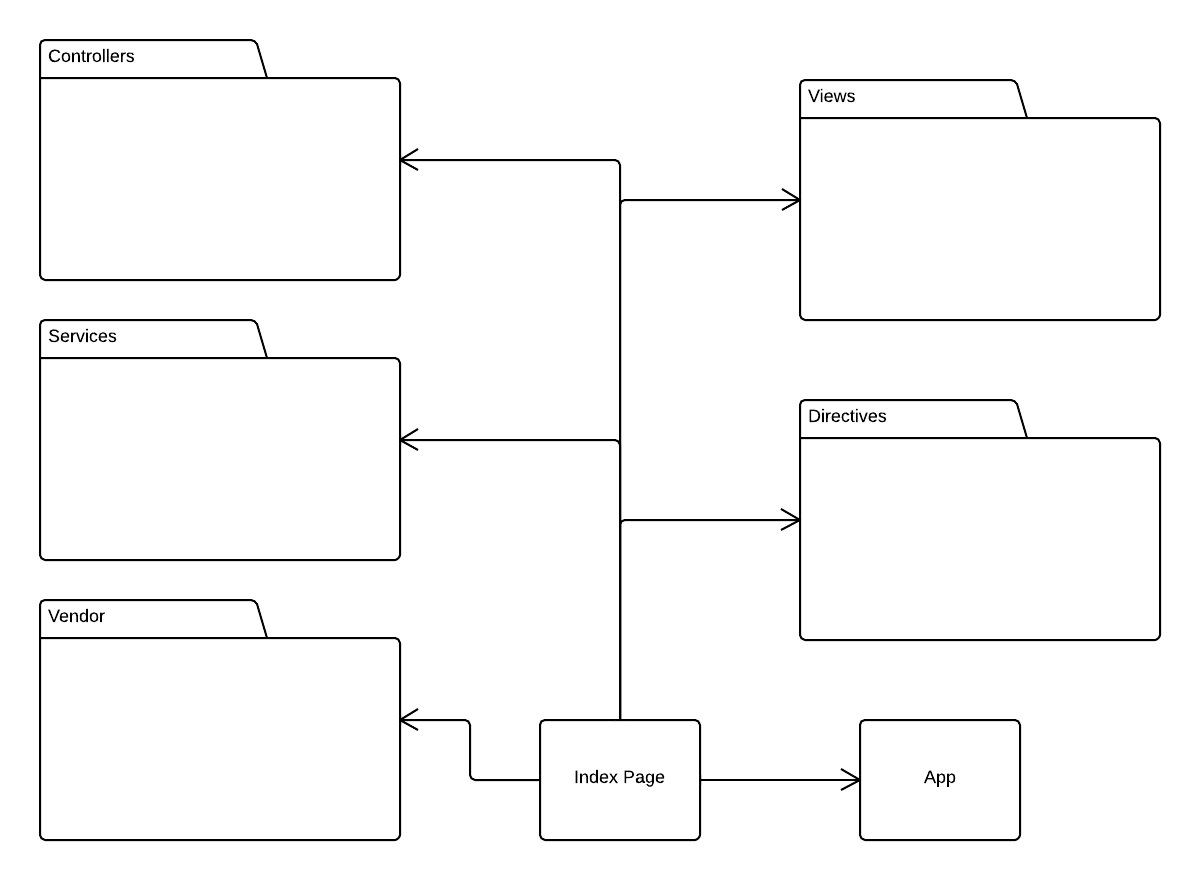
\includegraphics[width=0.8\linewidth]{./img/web-client-uml/subsystem-diagram}
\caption{Web client subsystem diagram.}
\label{fig:subsystem-diagram}
\end{figure}

\begin{center}
\begin{tabular}{|l|p{10cm}|}
\hline \multicolumn{2}{|c|}{\textbf{Services Subsystem}} \\
\hline \textbf{Module} & \textbf{Responsibility} \\ 
\hline httpInterceptor & Intercepts calls to the web service allowing for additional properties such as authentication tokens to be appended. Also sets the specific protocol that should be used to communicate with the web server. \\
\hline sessionUser & Stores a session user object that represents the user which is logged into the application. This module is used by controller modules to gain information about the current session user. This allows different views to be presented or different API methods to be called. \\
\hline
\end{tabular} 
\end{center}

\begin{figure}[H]
\centering
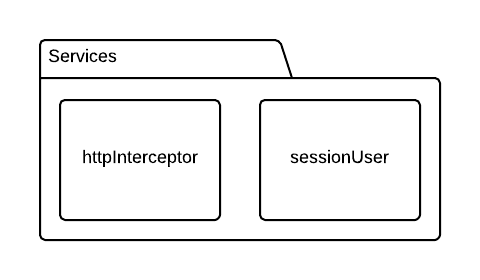
\includegraphics[width=0.8\linewidth]{./img/web-client-uml/services-subsystem-diagram}
\caption{Services subsystem of the web client.}
\label{fig:services-subsystem-diagram}
\end{figure}

\begin{center}
\begin{tabular}{|l|p{10cm}|}
\hline \multicolumn{2}{|c|}{\textbf{Directives Subsystem}} \\
\hline \textbf{Module} & \textbf{Responsibility} \\ 
\hline backImg & Displays the background image of walks shown in the \emph{all walks} view. \\
\hline hoverActive & Highlights the background of elements which are hovered over by the mouse. \\
\hline imageGallery & Applied to a DIV element to make nested image elements part of a carousel image gallery. \\
\hline imgSelector & Used in the image gallery view to give red outlines to selected media items. \\
\hline ladda & Applies loading spinners to buttons when an asynchronous request is taking place. \\
\hline loginValidator & Validates all input elements associated with the login form. Red or green borders are applied to elements if they are invalid or valid respectively. \\
\hline raty & Displays a star rating system for walk reviews. Takes an integer and represents it as the corresponding number of stars. \\
\hline regValidator & Validates all input elements associated with the registration form. Red or green borders are applied to elements if they are invalid or valid respectively. \\
\hline scroller & Applies a custom scroll bar to DIV elements that have overflowed. Overrides the default scroll bar style. \\
\hline userValidator & Validates fields associated with the user settings view. Red and green borders are given to inputs that are invalid or valid respectively. \\
\hline waypointValidator & Validates fields on the waypoint edit and add views. Gives input elements green or red borders if they are valid or invalid respectively. \\
\hline
\end{tabular} 
\end{center}

\begin{figure}[H]
\centering
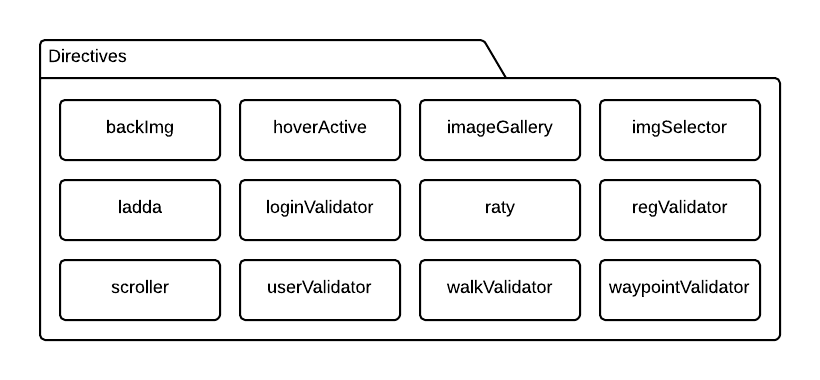
\includegraphics[width=0.8\linewidth]{./img/web-client-uml/directives-subsystem-diagram}
\caption{Directives subsystem of the web client.}
\label{fig:directives-subsystem-diagram}
\end{figure}

\begin{center}
\begin{tabular}{|l|p{10cm}|}
\hline \multicolumn{2}{|c|}{\textbf{Controllers Subsystem}} \\
\hline \textbf{Module} & \textbf{Responsibility} \\ 
\hline accountSettings & Retrieving the logged in user's current account settings and saving any new changes. \\
\hline addWalk & Adding a new walk including any associated waypoints to the database and validating walk attributes provided by the user. \\
\hline addWaypoint & Adding new waypoints to an existing walk including the uploading of any additional media such as images, audio or videos. \\
\hline alertModal & Provides a re-usable and customisable alert modal for use by any view controller. Controllers can inject custom messages and responses into this modal.\\
\hline allWalks & Retrieves all walks stored in the database for display on the \emph{all walks} view. \\
\hline editWalk & Updates existing walks with data provided by the user. \\
\hline editWaypoint & Updates existing waypoint information provided by the user including media modifications to images, videos and audio. \\
\hline editWaypointMedia & Manages media for both existing and new waypoints. Performs functions such as batch media removal and the uploading of new media items. \\
\hline login & Validates a user's log in credentials and creates a new user session if successful. \\
\hline myContributions & Accepts or rejects contributions made to the user's walks. Such contributions include the addition of new waypoints. \\
\hline myWalks & Retrieves a user's created walks for display on the \emph{my walks} view. \\
\hline navBar & Provides navigation to other views in the application such as \emph{all walks}, \emph{my walks}, the login modal and logout function. \\
\hline registerConfirm & Confirms the user's registration by displaying a modal displaying a success message. \\
\hline registerCtrl & Registers a new user account if the user has entered a valid set of account details. \\
\hline walkInfo & Retrieves walk information such as basic walk attributes, associated reviews, waypoints and media. \\
\hline waypointModal & Retrieves waypoint data for display within the waypoint modal when a map marker or waypoint list item is clicked. \\

\hline
\end{tabular} 
\end{center}

\begin{figure}[H]
\centering
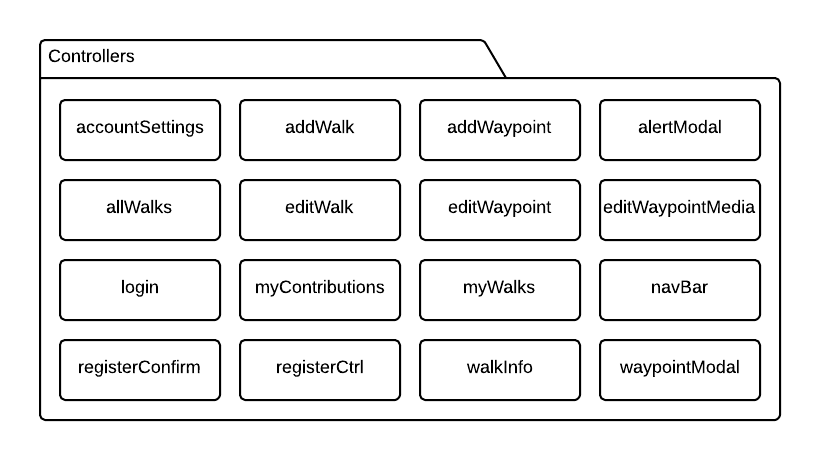
\includegraphics[width=0.8\linewidth]{./img/web-client-uml/controllers-subsystem-diagram}
\caption{Controllers subsystem of the web client.}
\label{fig:controllers-subsystem-diagram}
\end{figure}


\subsubsection{User Interfaces}
\label{sec:portal-user-interfaces}

This section presents and discusses the final user interfaces that were chosen for use in the web portal. These designs were the result of an iterative development process whereby the designs were shown to the client and revised according to suggested changes. They are also the result of interface enhancements designed to make the views more intuitive to users. The following sections will present a screen capture of each web portal view and discuss their functionality. The discussion for many of the interfaces remain the same as defined in the interim document and are cited as such.

\paragraph{Welcome View}\mbox{}\\
The welcome view shown in Figure \ref{fig:home} provides visitors with a link to download the Android application and instructs them to login or register account in order to use the portal. A footer has also been added to provide users with navigation links to important resources such as the Android application and \emph{About} page\cite{milestone2}.

\begin{figure}[H]

\centering

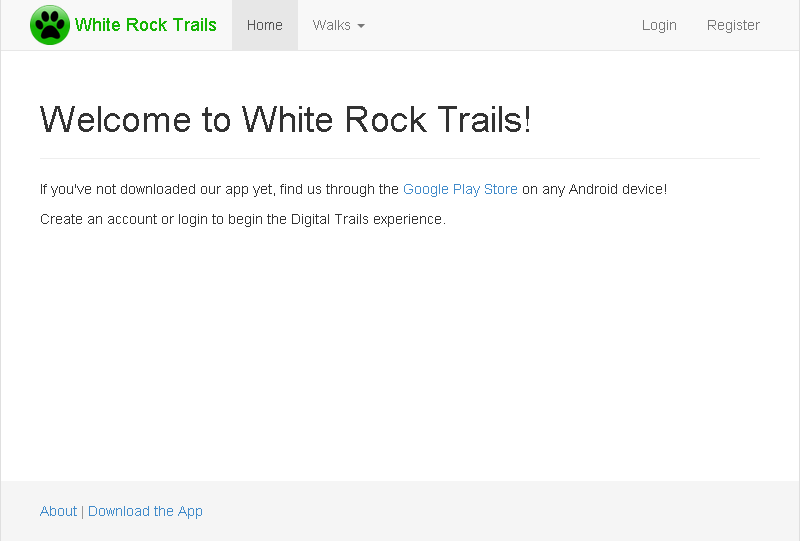
\includegraphics[width=0.8\linewidth]{./img/webportal/home}

\caption{Home view of the web portal.}

\label{fig:home}

\end{figure}



\paragraph{Responsive View}\mbox{}\\
Figure \ref{fig:home-responsive} demonstrates a responsive view of the web portal. This is the view that users will see when visiting the web portal on mobile devices such as smart phones and tablets. The responsive design minimizes the menu bar which can be expanded by clicking the button shown in the top right of the figure. In addition, web page content reduces in width and elements become stacked allowing for easier scrolling on mobile devices. The responsive design of the web portal is facilitated by the Bootstrap CSS and JavaScript library\cite{milestone2}. The items shown in the list feature navigational links to the associated pages. The \emph{Walks} item expands further child links which navigate to views that are associated with walks.



\begin{figure}[H]

\centering

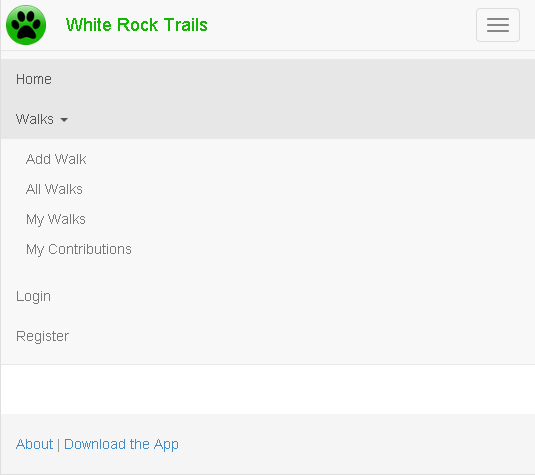
\includegraphics[width=0.6\linewidth]{./img/webportal/home-responsive}

\caption{Web portal responsive menu view.}

\label{fig:home-responsive}

\end{figure}



\paragraph{Login View}\mbox{}\\
Figure \ref{fig:login} shows the login view that users will see when they click on the \emph{Login} button in the top navigation bar. The login view displays as a modal in front of the web page. This will ensure that users do not have to navigate between pages in order to log in, thus enhancing usability. The login view requires users to input their email address and password followed by clicking the \emph{Login} button. The \emph{Login} button will display a spinner icon whilst the fields are validated to ensure the user is aware that the page is loading. An external validation library is used to validate the fields and display an error or success status. The library uses pre-defined validators to validate the structure of the email address and that the email and password pair is valid when checked against the White Rock Trails API. The validator changes the display of erroneous fields to feature red or green borders and tick or cross icons for invalid and valid fields respectively. A specific error message will also be displayed underneath erroneous fields to inform the reason for the error and allow users to amend it. When users successfully log in, the modal will close and the \emph{Login} and \emph{Registration} buttons shown in the top navigation bar are replaced with the user's full name\cite{milestone2}.



\begin{figure}[H]

\centering

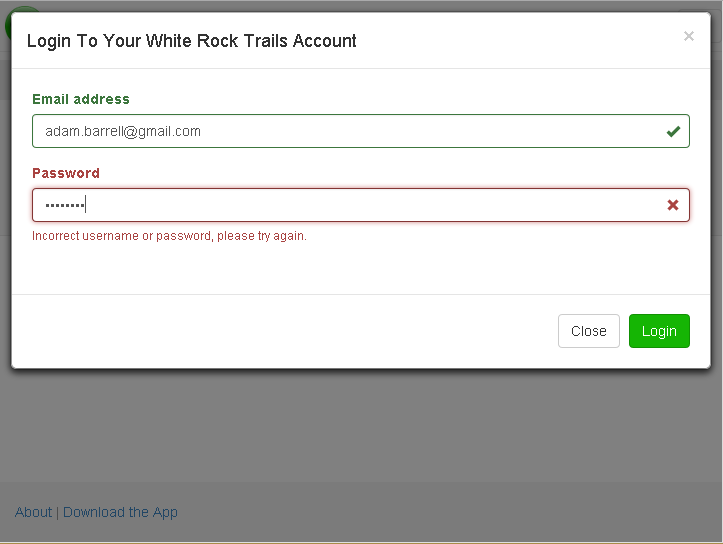
\includegraphics[width=0.7\linewidth]{./img/webportal/login}

\caption{Web portal login modal demonstrating validation.}

\label{fig:login}

\end{figure}



\paragraph{Registration View}\mbox{}
Figure \ref{fig:registration} shows the registration view that users will see when the \emph{Register} button is clicked in the top navigation bar. This view is also implemented as a modal for the same reasons as the login view and to maintain consistency throughout the application. The same validator is also used to validate the registration fields. However, inputs such as \emph{Email Address} and the two password fields require different validators. The former uses a validator that checks whether the provided email address has already been registered by another user. The latter checks whether the two passwords are identical. This will prevent users from registering using a mistyped password and subsequently not being able to log in. Clicking the \emph{Register} button will display a loading spinner inside as described for the login view. When users successfully register, they will be presented with a new confirmation modal instructing them to log in with their new account\cite{milestone2}.



\begin{figure}[H]

\centering

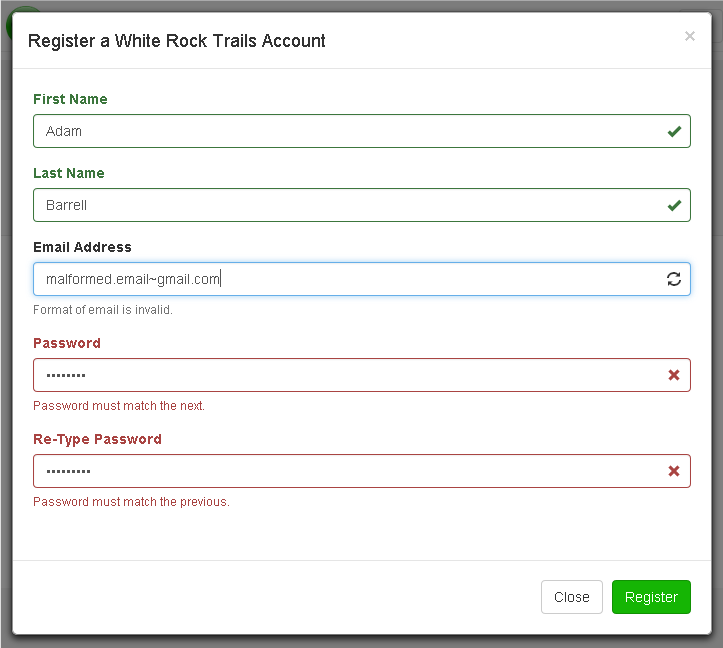
\includegraphics[width=0.7\linewidth]{./img/webportal/registration}

\caption{Web portal registration modal demonstrating validation.}

\label{fig:registration}

\end{figure}



\paragraph{All Walks View}\mbox{}\\
Figure \ref{fig:all-walks} shows the view users will see when they click on the \emph{Walks} button in the top menu bar and select the \emph{All Walks} option. This view displays a list of tiles, each representing a walk in the database. The background of each tile is an image selected from the collection of each walks way point images. Clicking a tile will navigate the user to a walk information view as presented in Figure \ref{fig:walk-info}\cite{milestone2}. 

Functionality for the \emph{Add Walk} button and search bar have been fully implemented since they were discussed in Milestone 2. Clicking the \emph{Add Walk} button navigates the user to a view where a new walk can be created. Entering text into the search box will perform a full text search of all walks held in the database. The search box also provides instantaneous results such that a request is sent to the server after a set time has expired after a user finishes typing. This allows for much faster and intuitive searching since the user is not required to press a button to execute the search. Finally, pagination has been implemented which allows users to view specific pages of search results that have overflowed the current view. A pagination control is present at the top and bottom of the \emph{All Walks} view for convenience to the user. Users can access specific results pages by clicking the relevant button index. 

\begin{figure}[H]

\centering

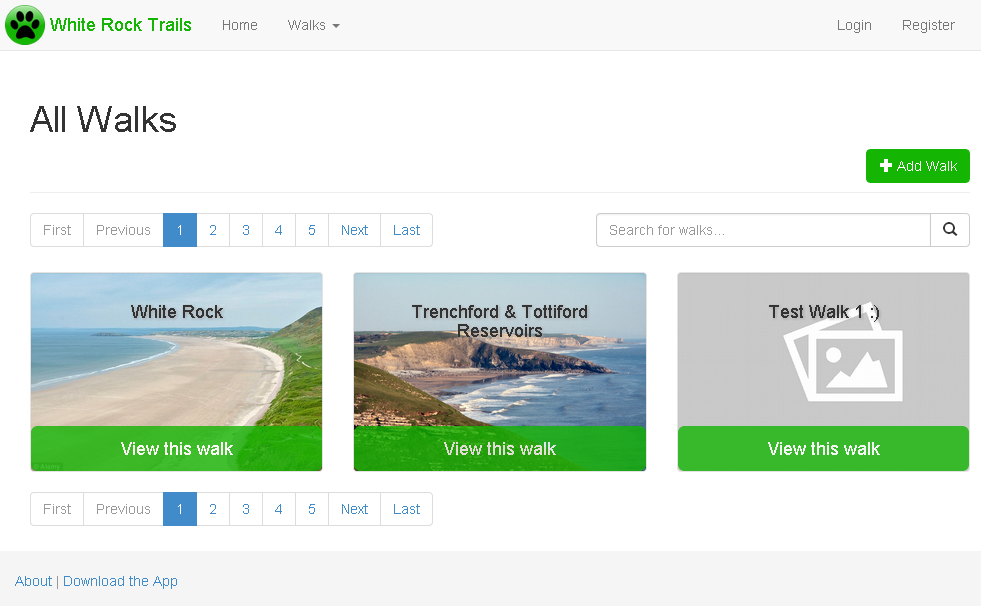
\includegraphics[width=1\linewidth]{./img/webportal/all-walks}

\caption{All walks view of the web portal.}

\label{fig:all-walks}

\end{figure}

\paragraph{Walk Information View}\mbox{}\\
Figure \ref{fig:walk-info} shows the view that a walk owner will see when they click on a walk owned by them from the \emph{All Walks} view. As shown in the figure, walk information will be displayed in this view such a title, description, duration, distance, difficulty rating and author. Navigation tabs above this information allow users to navigate between the \emph{Waypoints}, \emph{Reviews} and \emph{Walk} views. If any waypoint contributions have been submitted to the walk by other users, a \emph{Contributions} tab will appear. The number of pending contributions is also shown adjacent to the tab name. 

The interface also features \emph{Edit} and \emph{Delete} walk buttons which are only visible to the owner of the walk. Clicking the \emph{Edit} button will navigate the user to a view where the walk can be edited, whilst the \emph{delete} will prompt the user to confirm walk deletion. Walk data is asynchronously loaded from the database through the API. The Google Maps API is used to display the map shown in the right of the figure. The Google Maps API allows markers to be placed at specific GPS locations contained within the walk data. The map allows users to scroll and zoom around the walk area to gain an understanding of its location.

\begin{figure}[H]

\centering

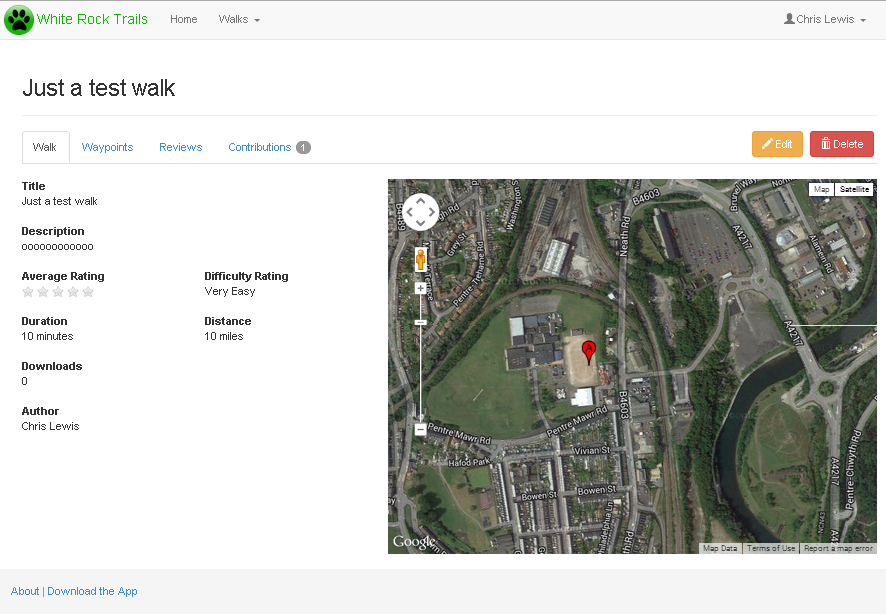
\includegraphics[width=1\linewidth]{./img/webportal/walk-info}

\caption{Walk information view of the web portal.}

\label{fig:walk-info}

\end{figure}

\paragraph{Walk Waypoints View}\mbox{}\\
Figure \ref{fig:walk-waypoints} shows the view that users will see when they click on the \emph{Waypoints} tab of the walk information view. The view shows the list of waypoints that are represented by markers on the map. Markers on the map can be identified by their letter index which references a waypoint shown in the leftmost list list. Clicking a list item or its corresponding map marker will display a modal containing media uploaded to the way point such as images, videos and audio. This feature has been fully implemented since Milestone 2. Finally, a visual fading effect has been applied to the waypoints list where an overflow is present. This indicates to the user that the list panel can be scrolled to display further waypoints.

\begin{figure}[H]

\centering

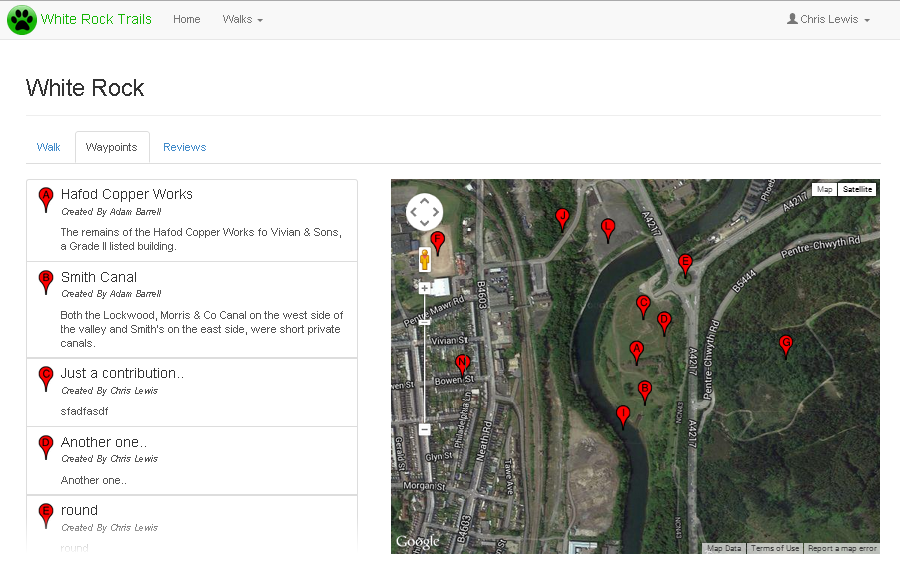
\includegraphics[width=1\linewidth]{./img/webportal/walk-waypoints}

\caption{Walk way points view of the web portal.}

\label{fig:walk-waypoints}

\end{figure}

\paragraph{Waypoint View}\mbox{}\\
The waypoint view shown in Figure \ref{fig:waypoint} is displayed when a list item or map marker is clicked from the walk waypoints view discussed in the previous paragraph. This view shows a read only representation of waypoint information such as its title, description and uploaded media. If the walk author is viewing this modal, an \emph{edit} and \emph{delete} button will be shown at the bottom which allows them to modify the waypoint. 

Clicking the \emph{edit} button will hide the current modal and display the waypoint in edit mode. Clicking the \emph{delete} button will prompt the user before permanently removing the waypoint from the walk. Clicking the final \emph{add image, audio or video} square in the gallery will allow the user to choose a file from their computer to be uploaded. Once chosen, the user will be required to enter a caption for the media. Upon specifying a caption, the media will be uploaded and added to the waypoint. 

Image and video media items are represented by a thumbnail image of their content. Since audio files do not have any visual representation, they have been given a gradient background featuring the caption above. The types of media displayed can be easily identified by an icon in the top left of each square. Clicking any media item will display a larger view the content and allow users to navigate backwards and forwards to previous and next media items respectively. This media viewer is presented in Figure \ref{fig:media-viewer}.

\begin{figure}[H]
\centering
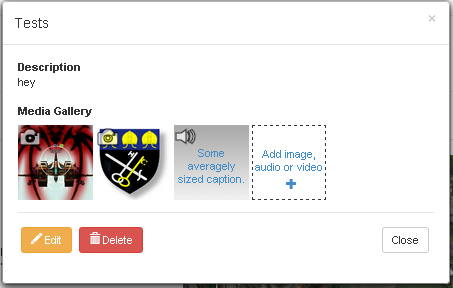
\includegraphics[width=0.7\linewidth]{./img/webportal/waypoint}
\caption{Walk waypoint view.}
\label{fig:waypoint}
\end{figure}

\begin{figure}[H]
\centering
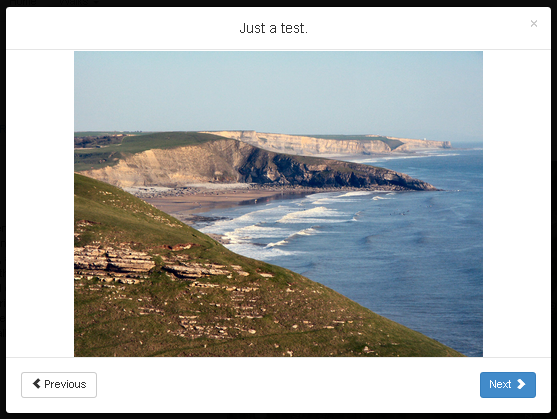
\includegraphics[width=0.7\linewidth]{./img/webportal/media-viewer}
\caption{Waypoint media viewer.}
\label{fig:media-viewer}
\end{figure}


\paragraph{Walk Reviews View}\mbox{}\\
Figure \ref{fig:walk-reviews} shows the view that users will see when they click the \emph{Reviews} tab from the navigation tabs bar. This view loads user reviews from the walk data and displays them in a list view as shown in the figure. A library called \emph{Raty} was used to generate the star rating system seen below the title of the review. It takes a review rating integer between 1-5 and generates a star representation\cite{milestone2}. Since Milestone 2, the review authors name now appears below the title so other users know who has created the review. In addition, authors of reviews will see a \emph{delete} button which can be clicked to remove their review. Walk owners will see the delete button on all reviews so to allow moderation.

Clicking the \emph{Add Review} button will hide the walk reviews and display a form which can be used to add a new one. When the user has submitted the new review, the list will re-appear and the form hidden.

\begin{figure}[H]
\centering
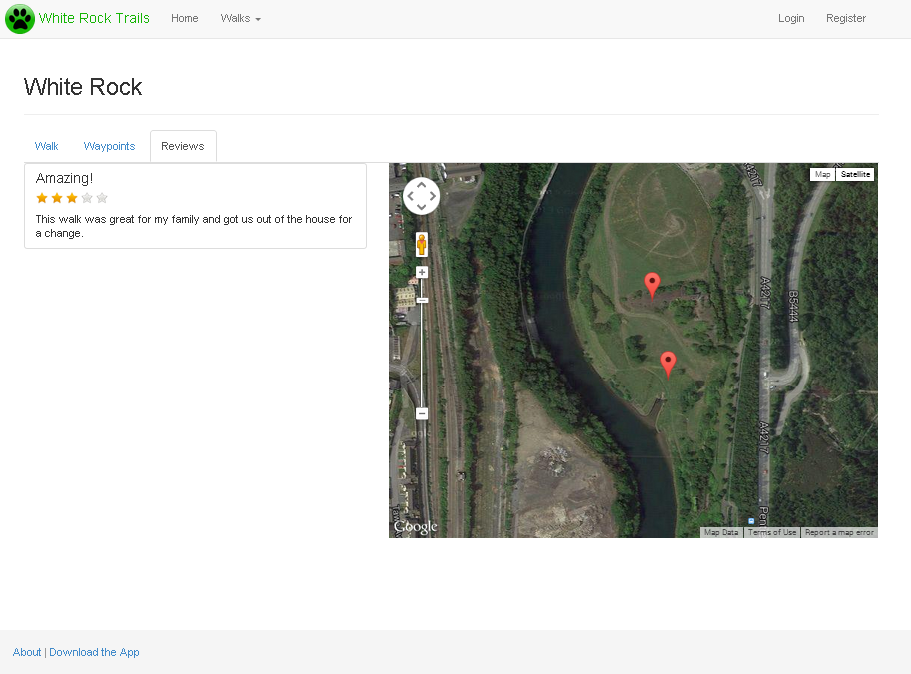
\includegraphics[width=1\linewidth]{./img/webportal/walk-reviews}
\caption{Walk reviews view of the web portal.}
\label{fig:walk-reviews}
\end{figure}

\paragraph{Waypoint Contributions View}\mbox{}\\
Since Milestone 2, an additional view has been added to allow walk authors to moderate waypoint contributions from other users. These will be displayed in a list as shown in Figure \ref{fig:waypoint-contributions}. Clicking a list item will present a modal displaying information about the waypoint that has been contributed. Each item has an \emph{accept} and \emph{reject} button to add the waypoint to the walk, or discard it respectively. Clicking either of these buttons will remove the contribution from the list and add a marker to the map representing its location.

\begin{figure}[H]
\centering
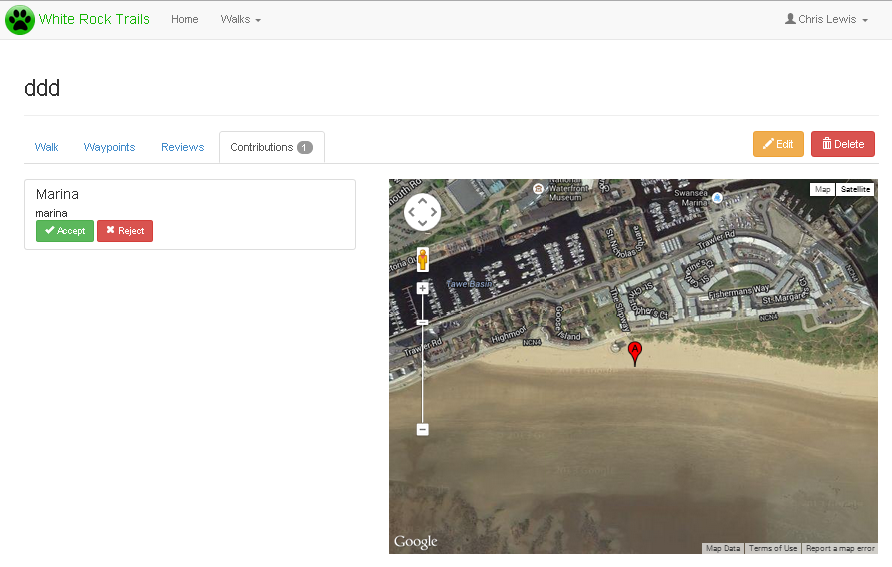
\includegraphics[width=1\linewidth]{./img/webportal/waypoint-contributions}
\caption{Waypoint contributions view.}
\label{fig:waypoint-contributions}
\end{figure}

\paragraph{Add Walk View}\mbox{}\\
The add walk view presented in Figure \ref{fig:add-walk} allows any user to create a new walk with associated waypoints. This view can be accessed from a link in the top navigation bar. Walk attributes can be entered and saved in the leftmost panel by clicking the \emph{save} button. The form can also be reset by clicking the \emph{undo} button. The \emph{cancel} button will discard the new walk and navigate back to the all walks view. The form also features client side error checking on saving, whereby erroneous fields are highlighted with a red border before the walk can be created. Waypoints can be added to the new walk by clicking on a map location. This will display the \emph{Add Waypoint} view discussed in the next paragraph.

\begin{figure}[H]
\centering
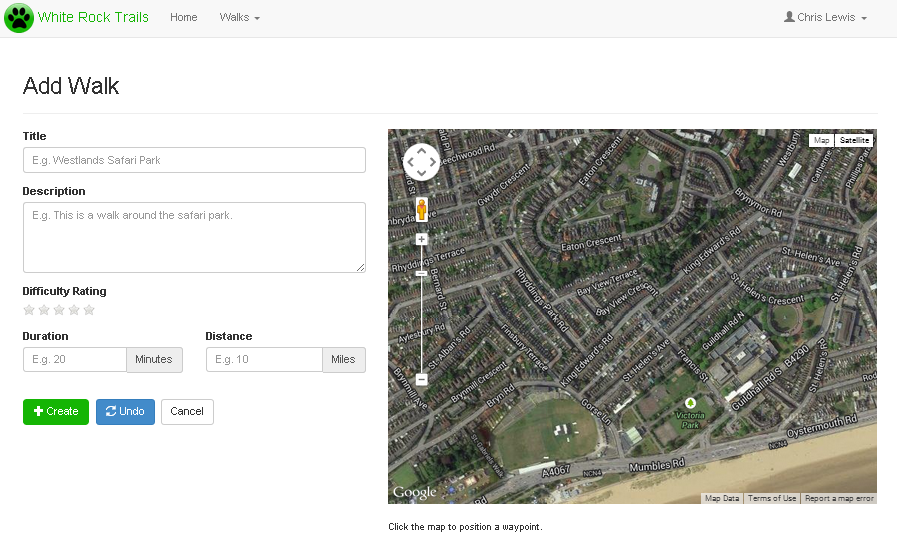
\includegraphics[width=1\linewidth]{./img/webportal/add-walk}
\caption{Add walk view.}
\label{fig:add-walk}
\end{figure}

\paragraph{Add Waypoint View}\mbox{}\\
The add waypoint view is presented in Figure \ref{fig:add-waypoint} and allows users to specify attributes of the waypoint to be created, including its \emph{title}, \emph{description}, \emph{latitude}, \emph{longitude}, \emph{visit order} and media. Clicking the \emph{Create} button will validate all fields and close the modal if successful. The waypoint will then be added to the new walk and a marker will appear on the map featured in the add walk view. Clicking the \emph{Manage} button will display an additional modal where media such as images, audio and videos can be added to the waypoint.

\begin{figure}[H]
\centering
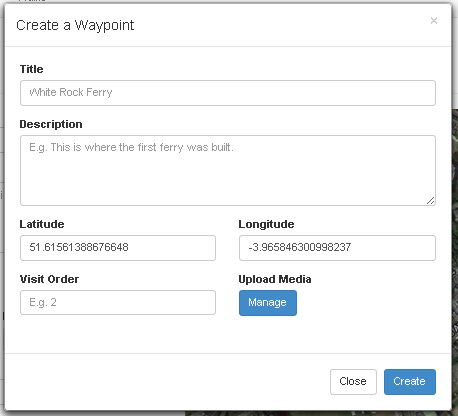
\includegraphics[width=0.7\linewidth]{./img/webportal/add-waypoint}
\caption{Add waypoint view.}
\label{fig:add-waypoint}
\end{figure}


\paragraph{Waypoint Media Gallery}\mbox{}\\
The waypoint media gallery shown in Figure \ref{fig:media-gallery} allows walk authors to manage the media which has been added to waypoints along their walks. Walk authors can select individual media items and click the \emph{delete selected} button to remove them in batch. Items selected for deletion are highlighted by a red border. The \emph{delete selected} button is only enabled when one or more media items are selected. On deleting media, they will be removed from the list and the \emph{delete selected} button disabled.

\begin{figure}[H]
\centering
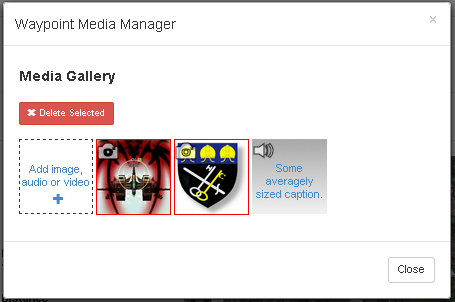
\includegraphics[width=0.7\linewidth]{./img/webportal/media-gallery}
\caption{Waypoint media gallery.}
\label{fig:media-gallery}
\end{figure}

\paragraph{Account Settings View}\mbox{}\\
The account settings view presented in Figure \ref{fig:user-account} allows registered users to modify their account details such as their \emph{first name}, \emph{last name}, \emph{email} and \emph{password}. All inputs are validated when the \emph{save} button is clicked. If any fields are invalid, they are given a red border to indicate this. Otherwise, a confirmation message is displayed above the account details to show the save has been successful.

\begin{figure}[H]
\centering
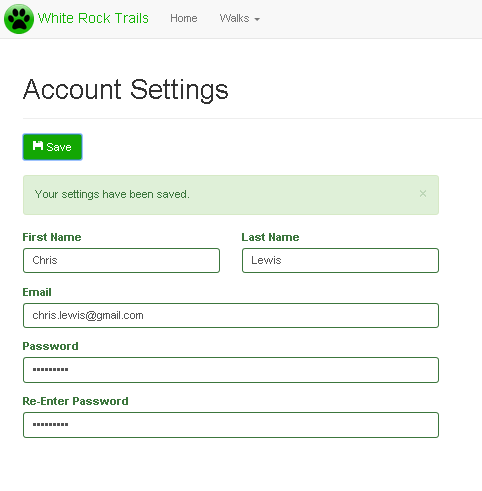
\includegraphics[width=0.7\linewidth]{./img/webportal/user-account}
\caption{User account settings view.}
\label{fig:user-account}
\end{figure}


\section{Android Application}
\label{sec:android-design}

\subsection{Technology Choices}
This section will discuss the choices of technology that were used to implement the application. These technologies were chosen for this project because both proved to be beneficial or essential to the development of the application. The following list will give the names of each technology and describe their purpose within the project.

\begin{itemize}

\item \textbf{Evolus Pencil} - Evolus Pencil is an open-source GUI prototyping tool that allows for mockups to be easily created. Pencil was used to create the initial prototype interface designs.

\item \textbf{Eclipse} - Eclipse is an integrated development environment that allows for the creation and development of applications. Eclipse was used to create the prototype designs for numerous interface iterations and the development of application functionality.

\end{itemize}

\subsection{Rejected Designs}
\label{sec:rejected-designs}

Through-out the course of the project, many design iterations were carried out. As a result, numerous interface designs were modified, while several designs were made redundant for a variety of reasons. This section of the document will analyse rejected designs, highlighting the issues that led to their redundancy. Below is an example of how the interface designs have progressed through several stages of iteration.\\

\textbf{Choose a walk interface} - This example is the walk selection interface ``Saved Walks''. The first iteration took the form of a simple interface design (Figure \ref{fig:view_walk}). Created using Evolus Pencil, the interface included the majority of features set out by Milestone 1 requirements. Here, the user may select from a list of available walks. The main interface window presents the selected walk's name, geological location, description, length (miles) and number of walk waypoints. The interface also included a start button, allowing users to begin the walk in current view.

\begin{figure}[H]
    \centering
    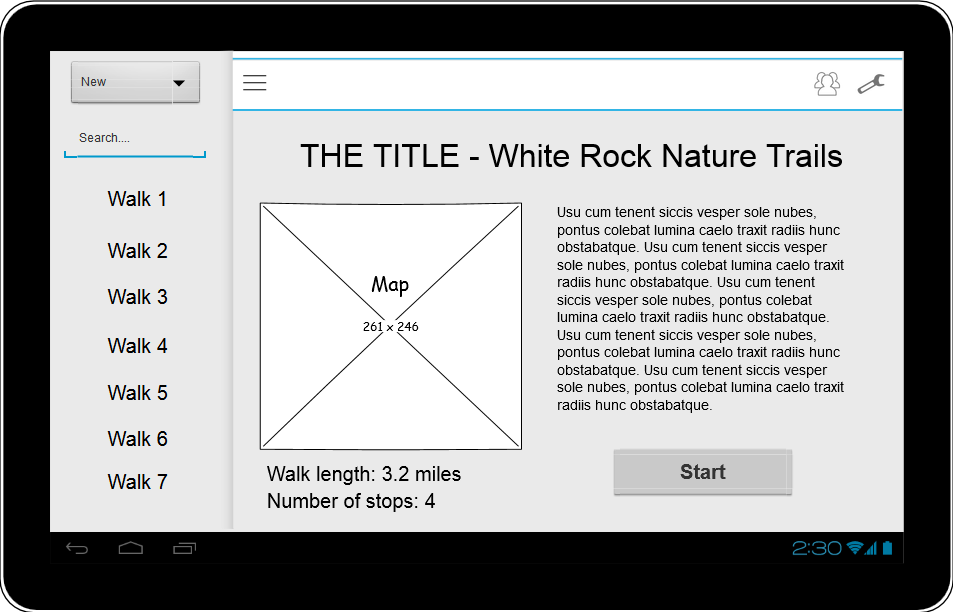
\includegraphics[width=0.8\textwidth]{chris/pencil_choose_walk}
    \caption{Walk selection interface - 1st iteration}
    \label{fig:choose_walk1}
\end{figure}

Based on the initial design, the interface was then created using Eclipse IDE [Cite]. This allowed for a more professional prototype design to be produced, illustrating how the final product may look. It was then possible to carry out improvements on the initial design. The \emph{combo-box} and \emph{search} features situated above the list of walks were removed. This was due to the fact they were better suited else where in the application, in a separate search interface. The removal of these two features now allowed for the list of walks to fill the entire side bar fragment. The final stage of this iteration was to add colour to the design. The chosen colour scheme for this iteration was a light shade of green to compliment the application logo. A small amount of shading was applied to the background colour of buttons and other features. 

\begin{figure}[H]
    \centering
    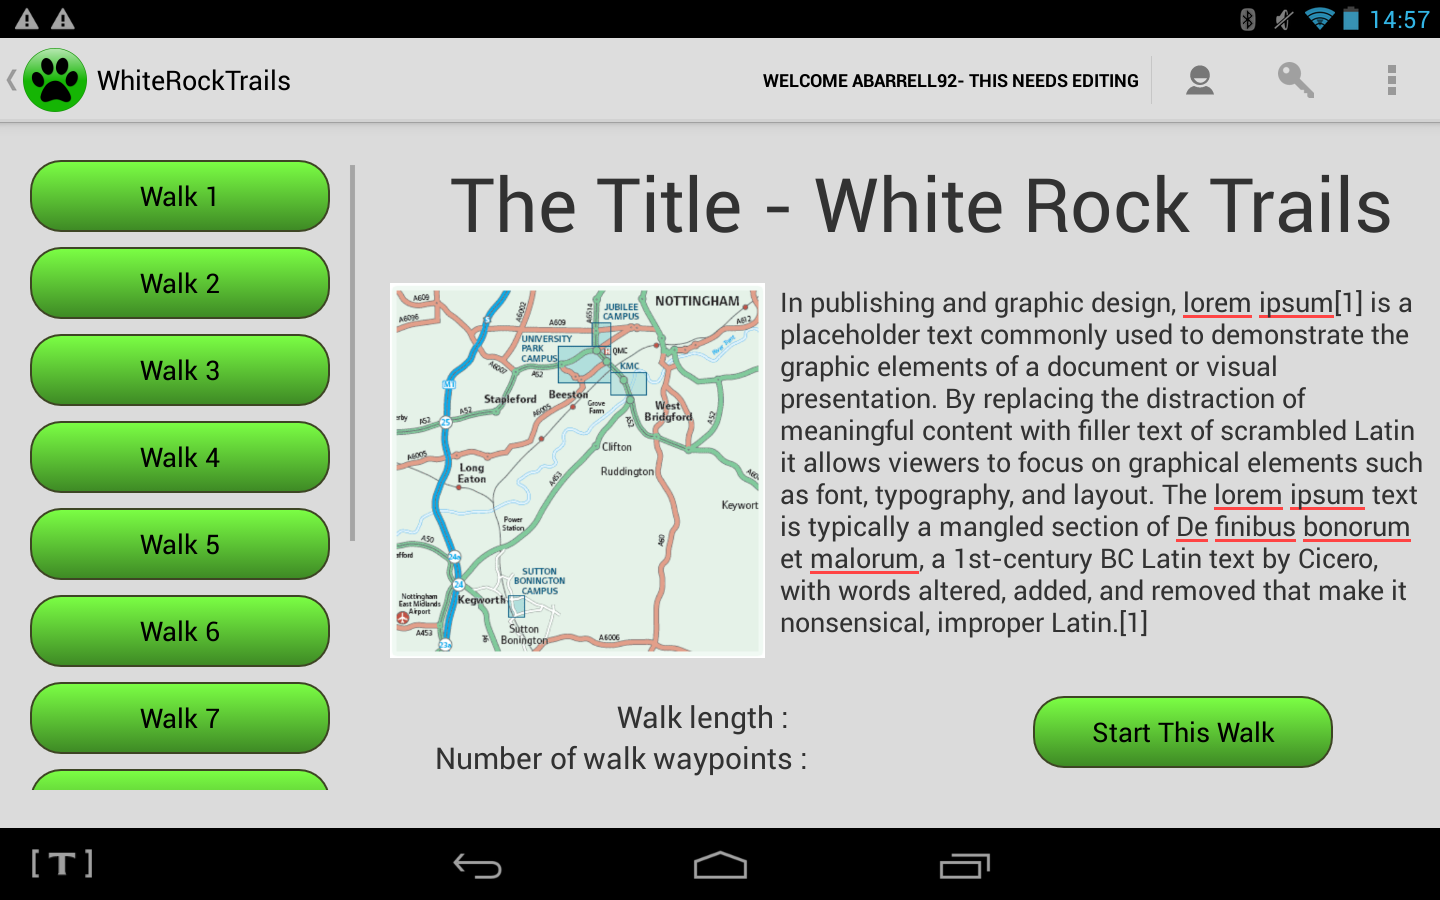
\includegraphics[width=0.8\textwidth]{chris/app_choose_walk}
    \caption{Walk selection interface - 2nd iteration}
    \label{fig:choose_walk2}
\end{figure}

The final iteration involved several layout alterations (Figure \ref*{fig:choose_walk3}). First, the list of walks fragment button style was removed. This was replaced by a walk list that was read from a database. The \emph{walk title} and \emph{description} are also now read from the database, and provide prompt text when the interface is first inflated. The \emph{start walk} button was raised to be aligned with the bottom of the walk map. Two additional features were also implemented. An \emph{average rating} star system was introduced along with a \emph{difficulty rating}. Both rating features are based on user feedback.

\begin{figure}[H]
    \centering
    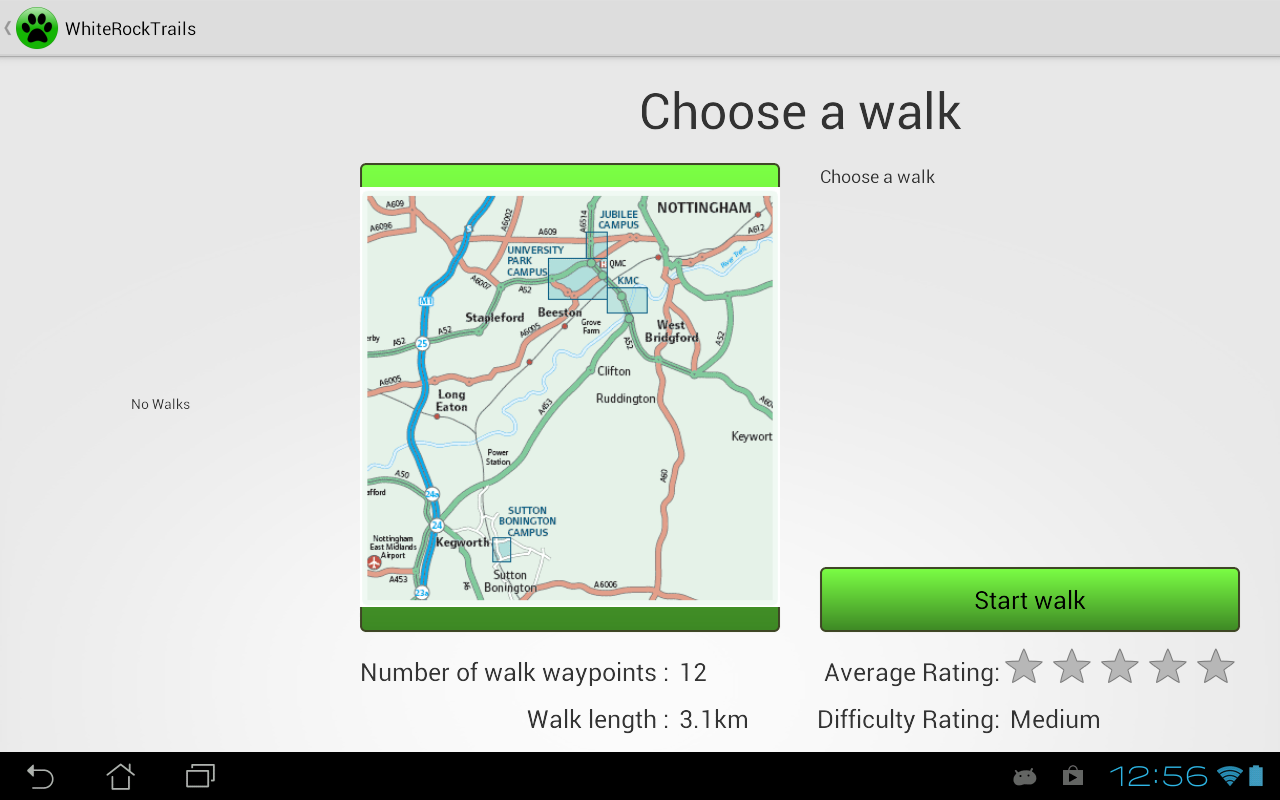
\includegraphics[width=0.8\textwidth]{chris/final_choose_walk}
    \caption{Walk selection interface - 3rd iteration EDIT THIS FOR WORKING MAP}
    \label{fig:choose_walk3}
\end{figure}


As previously documented, many interface designs were altered during the iteration stages of development. However, a small number of interface designs were fully rejected and re-designed. Below is a similar example of complete interface re-designs.\\

\textbf{My Walks interface} - The second design iteration saw the ``My Walks'' interface (Figure~\ref{fig:app_my_walks_view1}) present each walk create by the user in list form. Each walk included an \emph{ID}, \emph{title}, \emph{edit} and \emph{delete} button. The user also had the ability to create a new walk from this interface. During evaluation, it was decided that the proposed interface was not suitably designed. It's inappropriate layout meant that the only information available about each walk was in fact its ID and title. Before selecting the edit or delete button, the user may have to view a walk if they were unable to recall by name. The list format also led to a poor use of layout positioning. A vast amount of empty space was visible, especially when using the application on a large tablet.

\begin{figure}[H]
    \centering
    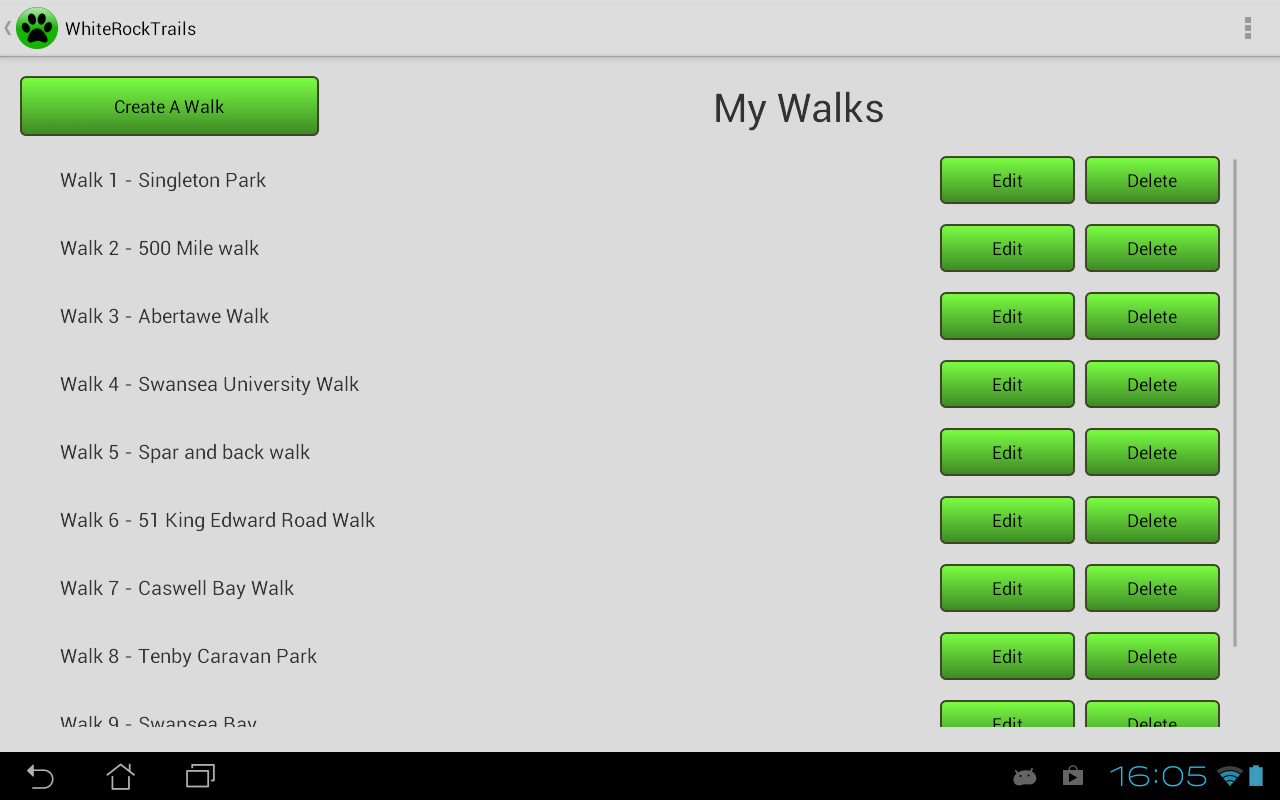
\includegraphics[width=0.8\textwidth]{chris/app_my_walks_view}
    \caption{My Walks interface - 2nd iteration}
    \label{fig:app_my_walks_view1}
\end{figure}

With the above negative aspects of this design taken into consideration, a new interface design was produced (Figure \ref{fig:app_my walks_view2}). The interface now presents each walk in a side-bar style list fragment, reading each walk from a database. The \emph{edit} and \emph{delete} buttons are included in the main fragment. Additional features to the interface now include the walk's \emph{geological location}, \emph{description}, \emph{length(in miles)}, \emph{number of walk waypoints}, \emph{difficulty rating} and \emph{average user rating}. Providing this level of information allows users to view a basic summary of each walk created by the user.\\

\begin{figure}[H]
    \centering
    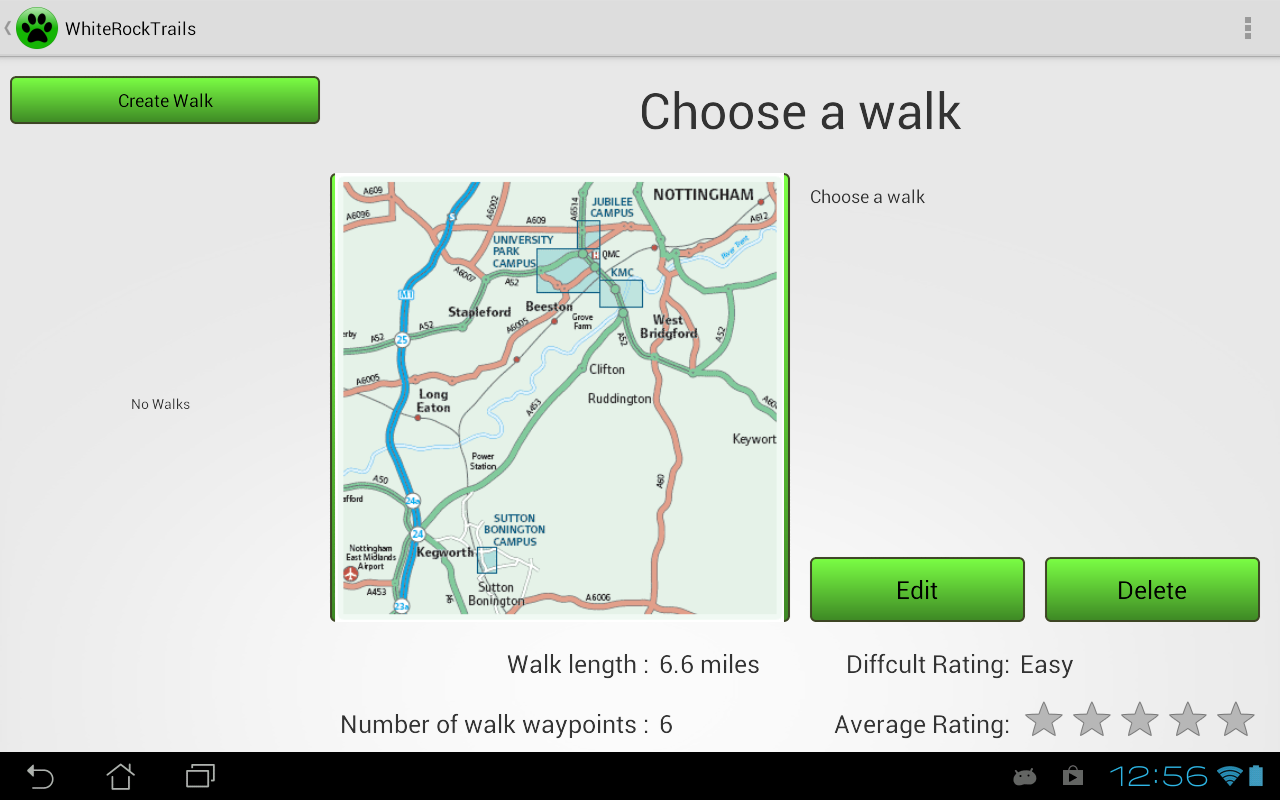
\includegraphics[width=0.8\textwidth]{chris/final_walk_view}
    \caption{My Walks interface - 3rd iteration}
    \label{fig:app_my walks_view2}
\end{figure}
% User Interface Design
% UML Diagrams
% Descriptions of each class
% Technology Choices

\subsection{Chosen Design}
\label{sec:chosen-designs}

This section presents and discusses the final user interfaces that were chosen for use in the application. These designs were the result of an iterative development process whereby the designs were shown to the client and revised according to suggested changes. They are also the result of interface enhancements, designed to make each interface more intuitive to users. The following sections will present a screen capture of each interface application and discuss their functionality.

\paragraph*{Splash Screen interface}\mbox{}\\ 

\begin{figure}[H]
    \centering
    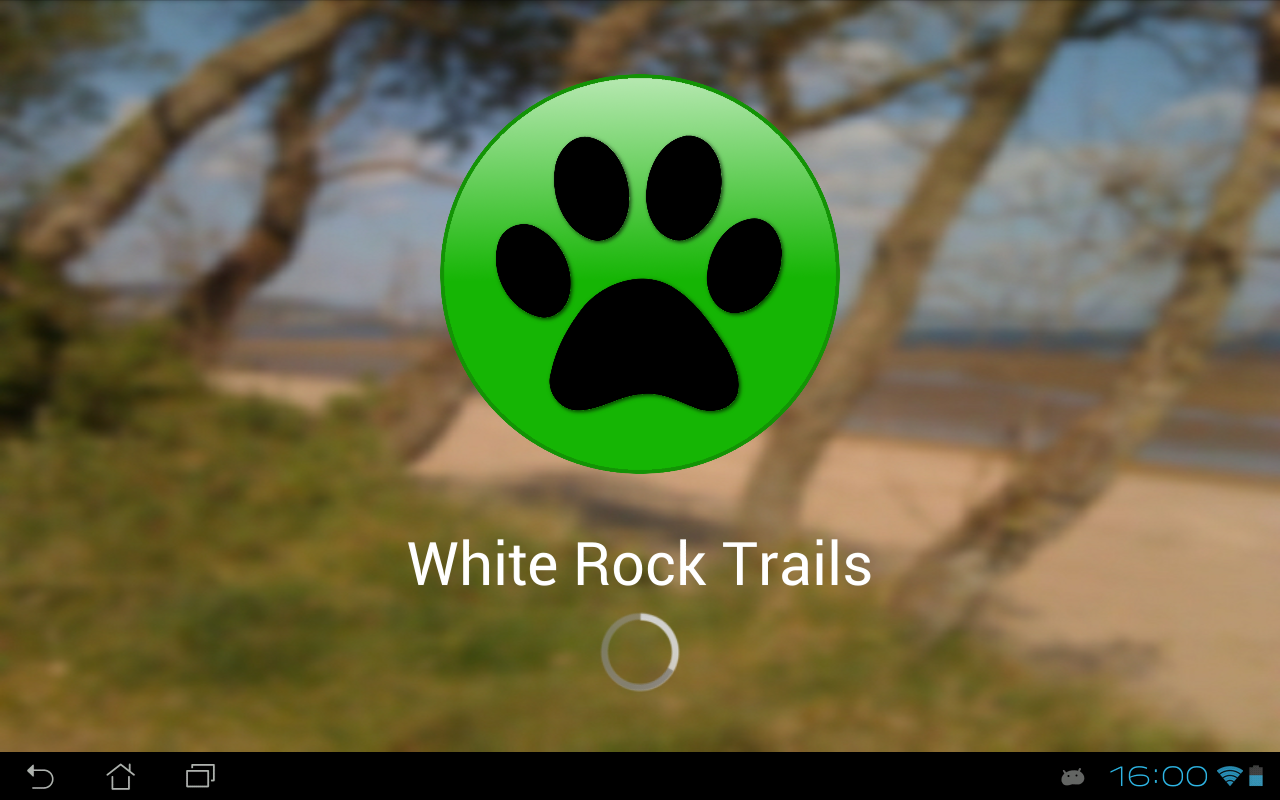
\includegraphics[width=0.8\textwidth]{chris/splash_screen}
    \caption{Splash Screen interface}
    \label{fig:splash_screen}
\end{figure}

The \emph{splash screen} is the first interface inflated when the application is opened. It includes the company logo, company name and a loading feature. After a short period of time, the \emph{launch} interface will inflate.

\paragraph*{Launch interface}\mbox{}\\
\begin{figure}[H]
    \centering
    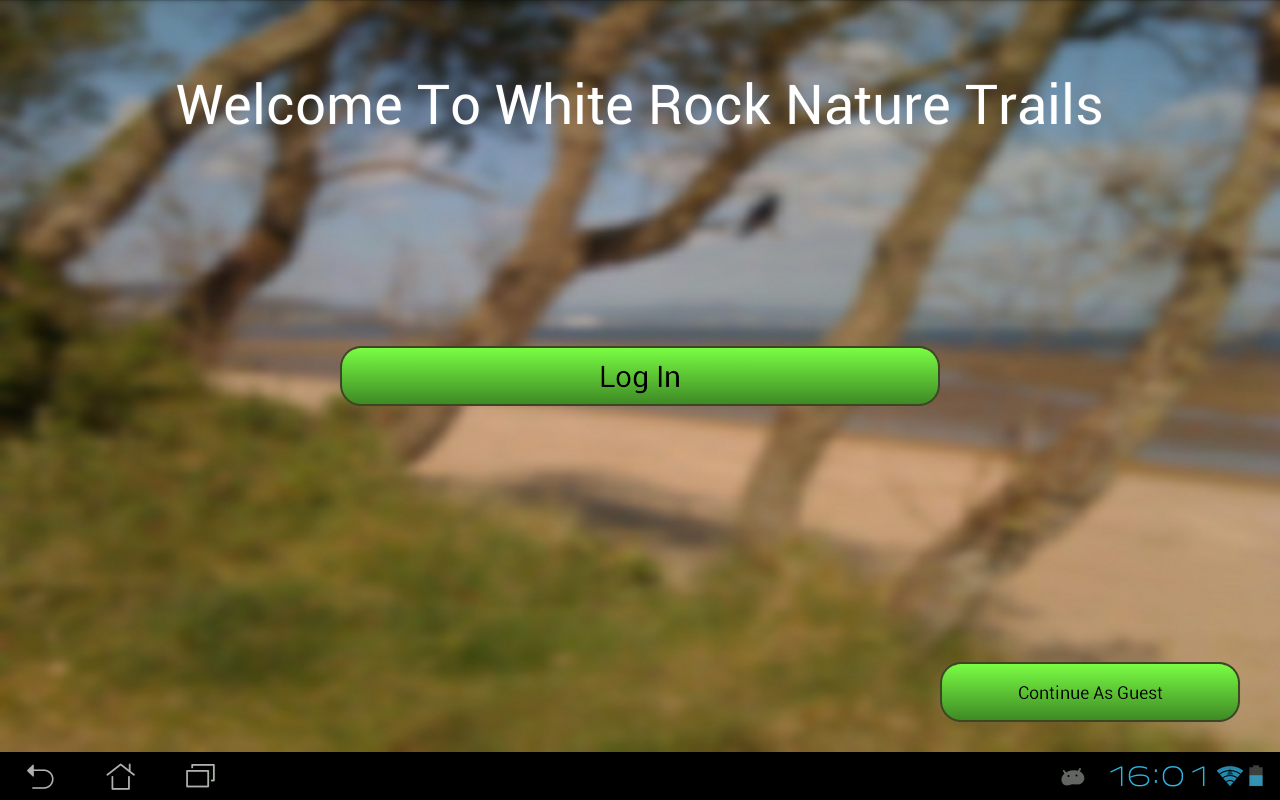
\includegraphics[width=0.8\textwidth]{chris/launch_view}
    \caption{Launch interface}
    \label{fig:launch_view}
\end{figure}

The \emph{launch} interface presents the user with an aesthetically pleasing layout. An edited image of the local beach is used as the background. At the top of the interface is a \emph{Text View} welcoming the user to the application. At the centre of the interface is a \emph{Log In}. Pressing the \emph{Log in} button will navigate to the \emph{Log In} interface. A \emph{Continue as guest} button is also situated at the bottom right corner. Pressing this button will by-pass the log in feature and take the user directly to the \emph{Home} interface but with limited privileges.

\paragraph*{Log In interface}\mbox{}\\

GET IMSGE \\

The \emph{Log In} interface presents the user with a welcome message fixed to the top, along with prompt text directly below. The focus of this interface is the \emph{email} and \emph{password} text boxes. Selecting either text box will inflate a keypad, where the user may enter log in details. Below is a \emph{Sign In} button and a \emph{New user?} text view. If valid details are entered, pressing the \emph{Sign In} button will navigate to the \emph{Home} interface. If invalid details are entered, a pop-up dialogue will notify users that the log in attempt has failed. Pressing the \emph{New user?} text view will navigate to the \emph{Register} interface, where the user may register a new account.

\paragraph{Register interface}\mbox{}\\
INSERTT IMAGE\\

The \emph{Register} interface presents the user with a series of edit text boxes, where details such as \emph{first name, last name, email address} and \emph{password} can be entered in order to create a new account. Below this is a \emph{Create Account} button and an \emph{Already a member?} text view. If suitable details are entered, pressing the \emph{Create Account} button will create a user account and navigate to the \emph{Home} interface. If unsuitable, the account creation will be rejected.

\paragraph*{Home interface}\mbox{}\\

\begin{figure}[H]
    \centering
    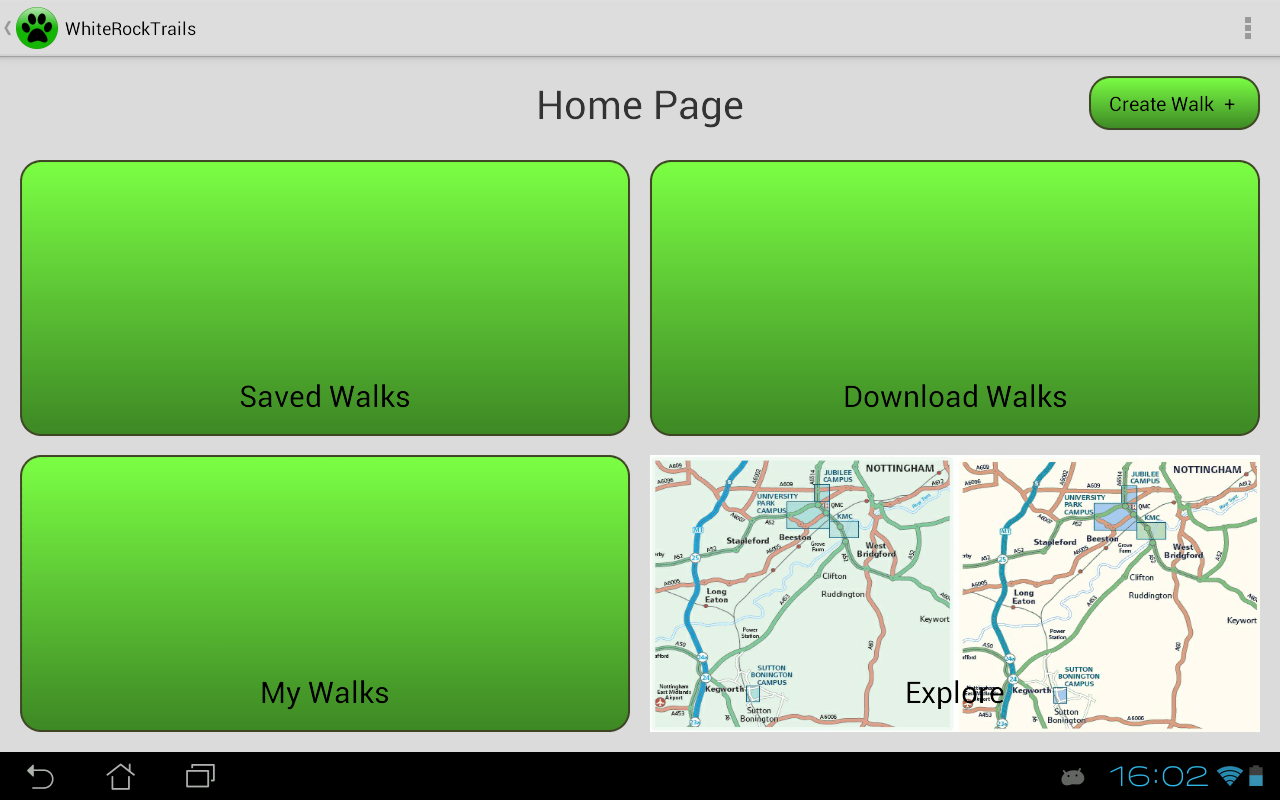
\includegraphics[width=0.8\textwidth]{chris/home}
    \caption{Home interface}
    \label{fig:home}
\end{figure}

The \emph{Home} interface is the central focus point of the application. This interface includes a title and a grid of four navigation buttons; a \emph{Saved Walks}, a \emph{Download Walks}, a \emph{My Walks} and an \emph{Explore} button. Pressing on any button will navigate to the respective interface.

\paragraph*{Saved Walks interface}\mbox{}\\
\begin{figure}[H]
    \centering
    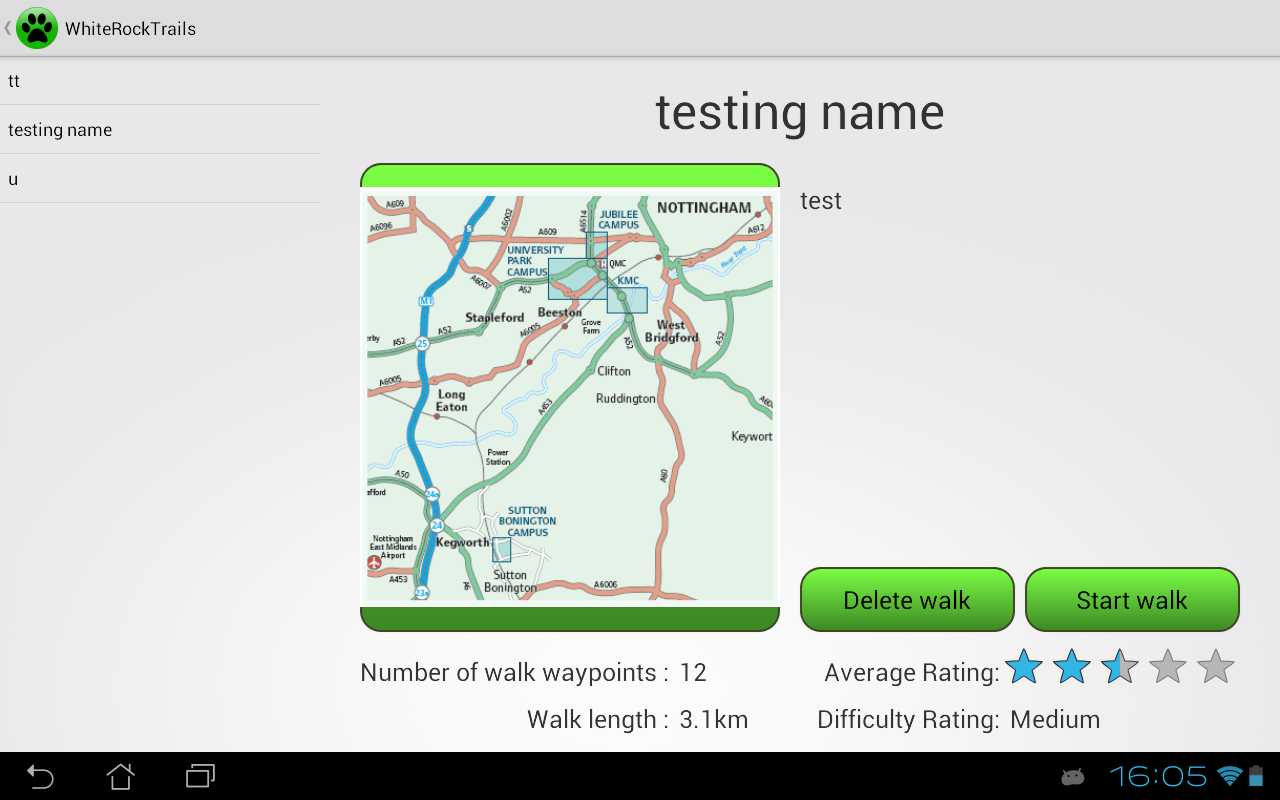
\includegraphics[width=0.8\textwidth]{chris/saved_walks}
    \caption{Saved Walks interface}
    \label{fig:saved_walks}
\end{figure}

The \emph{Saved Walks} interface presents a list of all saved walks on the left hand side. Pressing an element within the list will show the details of that walk. The main interface window displays the \emph{walk title, description, geological location} map and a \emph{start} button. Pressing the \emph{start} button will inflate a map interface and begin the walk trail.

\paragraph*{My Walks interface}\mbox{}\\

\begin{figure}[H]
    \centering
    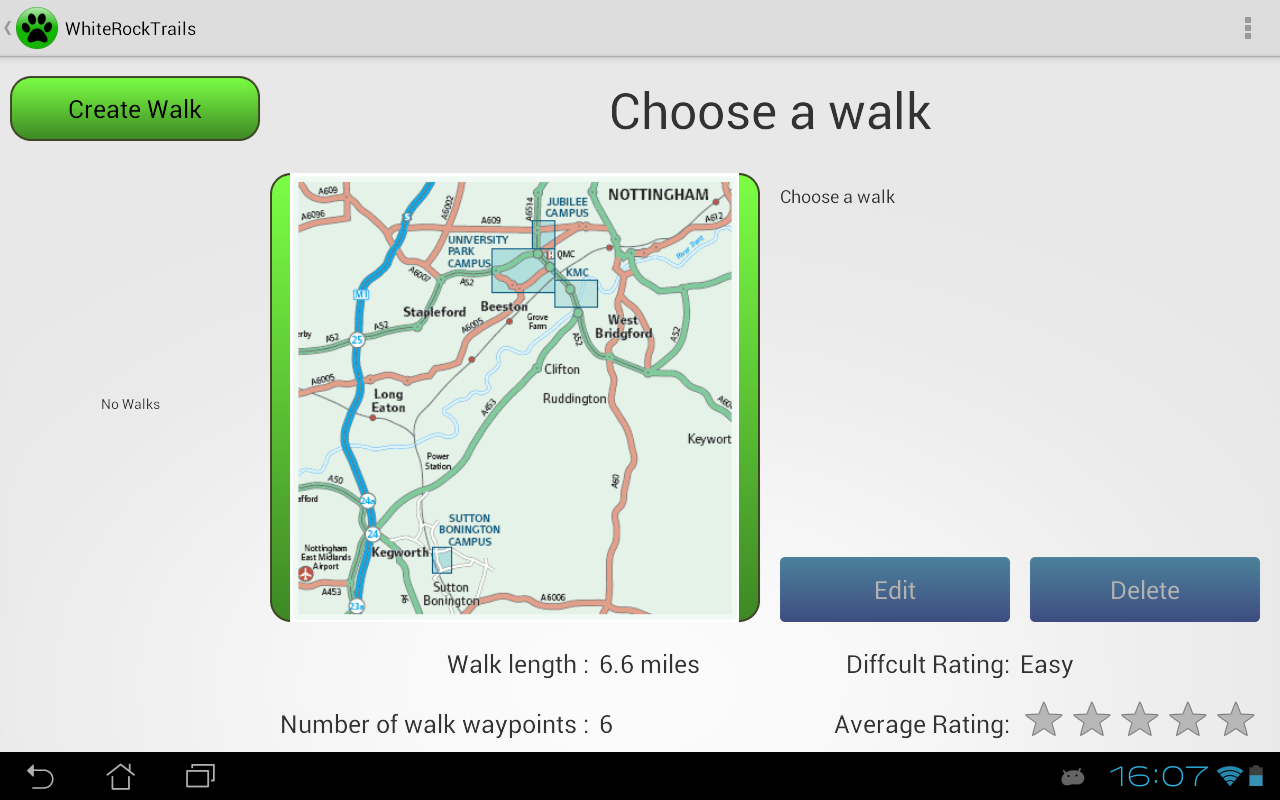
\includegraphics[width=0.8\textwidth]{chris/my_walks}
    \caption{My Walks interface}
    \label{fig:my_walks}
\end{figure}

The \emph{My Walks} interface is similar to that of the \emph{Saved Walks} layout with a few additional features. The left-hand side list of walks fragment now includes a \emph{Create Walk} button. Pressing this button will inflate a \emph{Create Walk} interface. Instead of the \emph{start} button, the interface now includes an \emph{edit} and \emph{delete} button. Pressing the \emph{edit} button will navigate to the \emph{Edit Waypoint} interface. Pressing the \emph{delete} button will inflate a pop-up dialogue, requiring the user to confirm or cancel the walk deletion. If \emph{confirm} is selected, the walk is deleted. If \emph{cancel} is selected, the pop-up dialogue will close.

\paragraph*{Download Walks interface}\mbox{}\\
\begin{figure}[H]
    \centering
    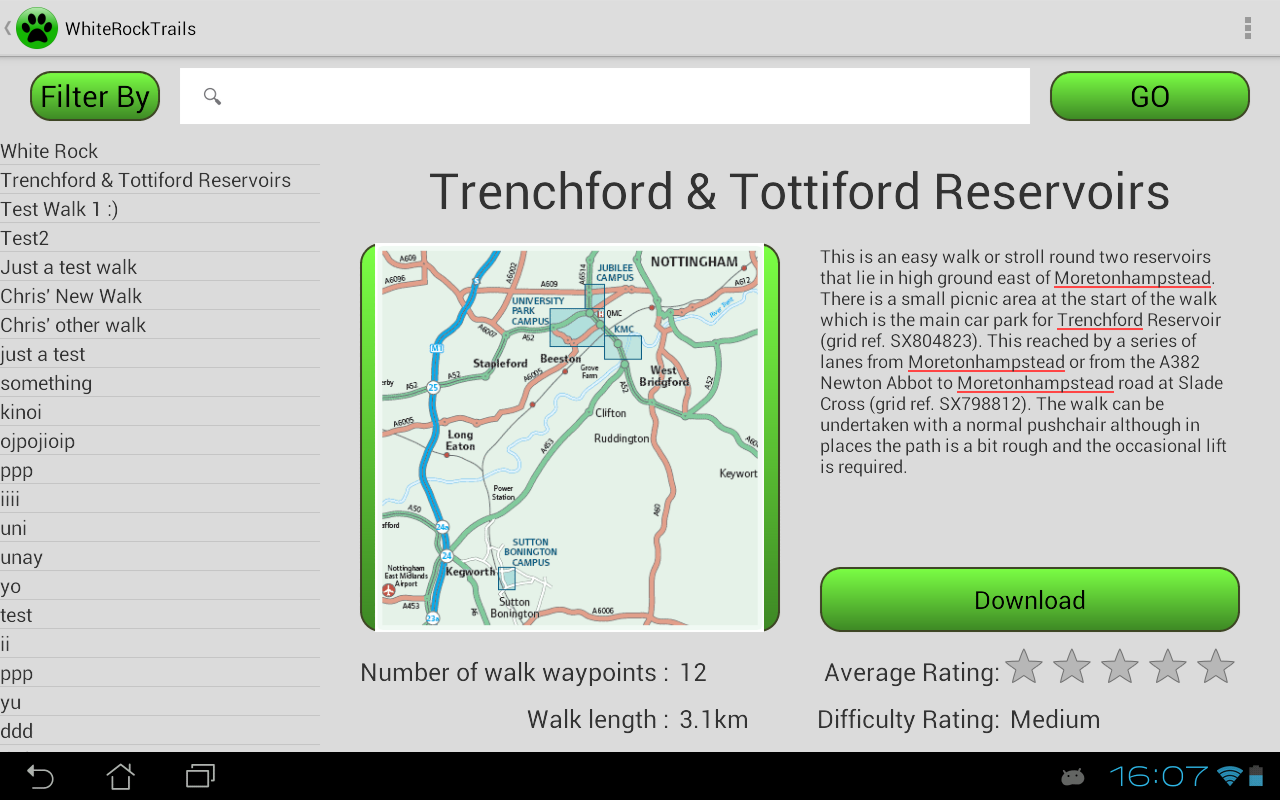
\includegraphics[width=0.8\textwidth]{chris/download_walk}
    \caption{Download Walks interface}
    \label{fig:download_walk}
\end{figure}

The \emph{Download Walks} interface allows users to search for walks and download them. The interface takes the layout form previously seen in \emph{My Walks} interface. The list of walks now consists of all possible walks taken from the database. A search text box at the top of the interface allows users to search for a particular walk or area. Selecting a walk from the list will present all walk details in the main interface window. Here the user may save that particular walk by pressing the \emph{Download walk} button.

\paragraph*{Explore interface}\mbox{}\\
\begin{figure}[H]
    \centering
    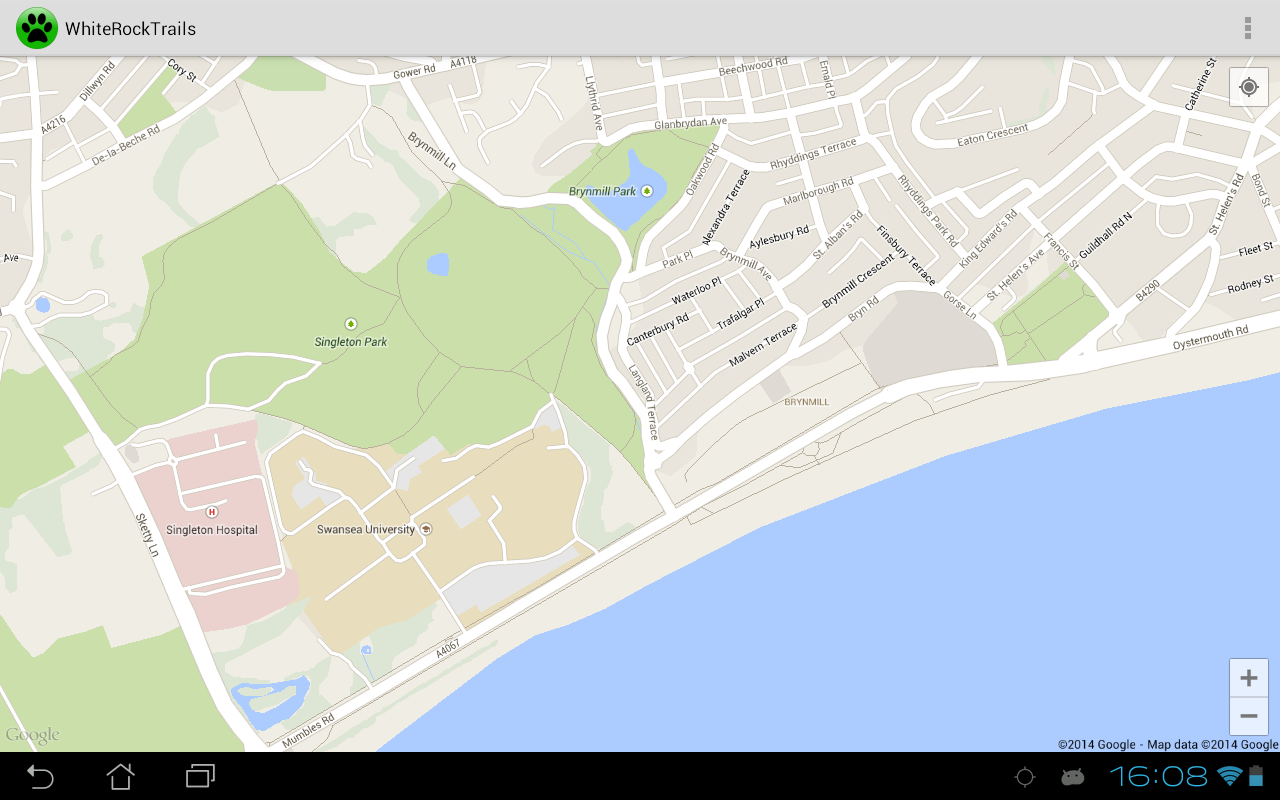
\includegraphics[width=0.8\textwidth]{chris/explore}
    \caption{Explore interface}
    \label{fig:explore_view}
\end{figure}

Unlike the majority of interface designs previously documented, the \emph{Explore} interface has a single purpose. It presents a world map, allowing users to move freely across the map, zooming in and out as desired. The explore interface acts as a form of ``location search''. This provides users with additional freedom to view any location and potentially discover new walk trails that could be created.

\paragraph*{Create Walk interface}\mbox{}\\
\begin{figure}[H]
    \centering
    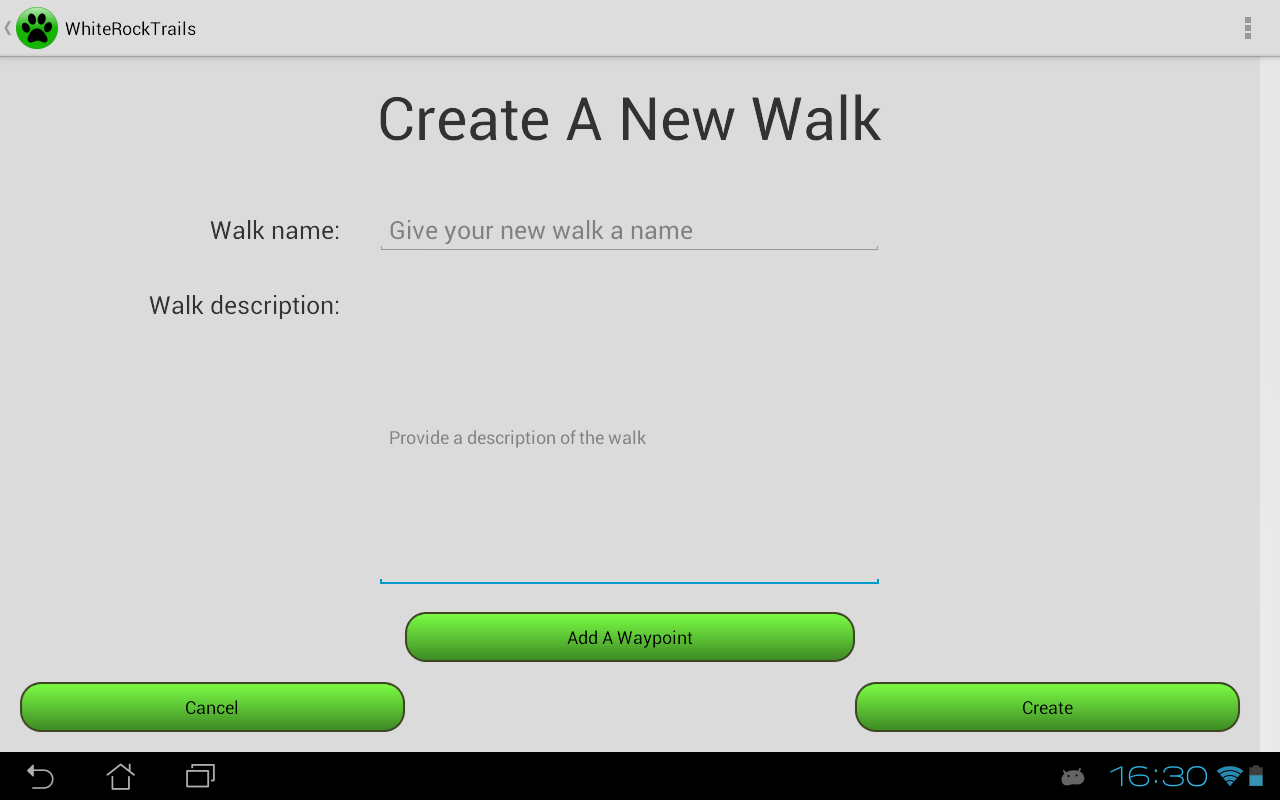
\includegraphics[width=0.8\textwidth]{chris/create_walk}
    \caption{Create Walk interface}
    \label{fig:create_walk}
\end{figure}

The \emph{Create Walk} interface has a basic layout. An title is positioned at the top of the interface. This is followed by a \emph{walk name} and a \emph{walk description} editable text box. Selecting either text box will allow for the respective walk information to be entered. The interface also includes an \emph{Add a waypoint} button, \emph{cancel} button and a \emph{create} button. Pressing the \emph{Add a waypoint} button will navigate to an \emph{Add Waypoint} interface. Pressing the cancel button will return to the previous interface, while the \emph{Create} button will create a new walk using the details entered by the user.

\paragraph*{View Walk interface}\mbox{}\\

INSERTT IMAGE\\

The \emph{View Walk} interface is inflated when the user wishes to view a walk and its waypoints. Similar to the explore view, the user may move around the map, zooming in and out as desired. When the user is within close proximity of a waypoint, a pop-u dialogue will appear on-screen. This dialogue will include the waypoint name, a short description and any relative media that has been attached to that waypoint. 

\paragraph*{Edit Walk interface}\mbox{}\\
INSERTT IMAGE\\

The \emph{Edit Walk} interface allows users to make changes to walks they created. The presented interface provides users with the ability to update main information such as walk name and description. Below this is an \emph{Add a waypoint} button and a \emph{edit waypoints} button. The user may add numerous waypoints and make changes to current waypoints. If no changes are to be made or saved, pressing the \emph{cancel} button will return to the previous interface. Pressing the \emph{save} button will save all changes and return to the \emph{My Walks} interface.

\paragraph{Add Waypoint interface}\mbox{}\\
\begin{figure}[H]
    \centering
    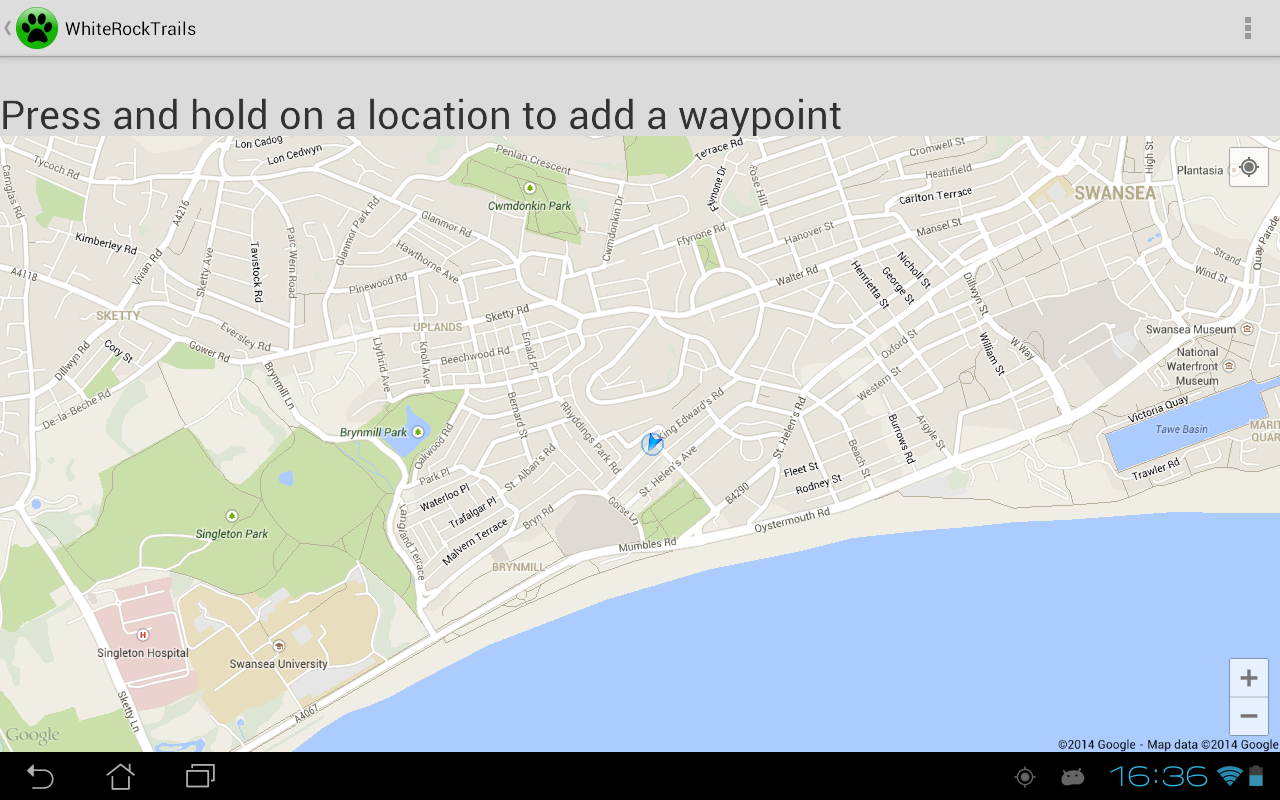
\includegraphics[width=0.8\textwidth]{chris/add_waypoint}
    \caption{Add Waypoint interface}
    \label{fig:edit_waypoint}
\end{figure}

The \emph{Add Waypoint} interface allows users to add a waypoint to a walk simply by selecting and holding on a position on the map provided. A text prompt is also included, providing users with instructions.

\paragraph{Edit Waypoint interface}\mbox{}\\


The \emph{Edit Waypoint} interface allows users to edit a waypoint of an existing walk. The user may edit the waypoint name, description and multimedia attached. When complete, pressing the \emph{save} button will save changes made and return to the \emph{edit walk} interface. Pressing the \emph{cancel} button will return to the \emph{edit walk} interface without saving any changes to that particular waypoint.

\paragraph*{Application Flow Diagram}\mbox{}\\

This section will present a flow diagram of the interface designs discussed previously. The figure \ref{fig:flow} helps illustrate the flow of the application and allows us to visualise how interfaces may depend on one another.

\begin{figure}[H]
    \centering
    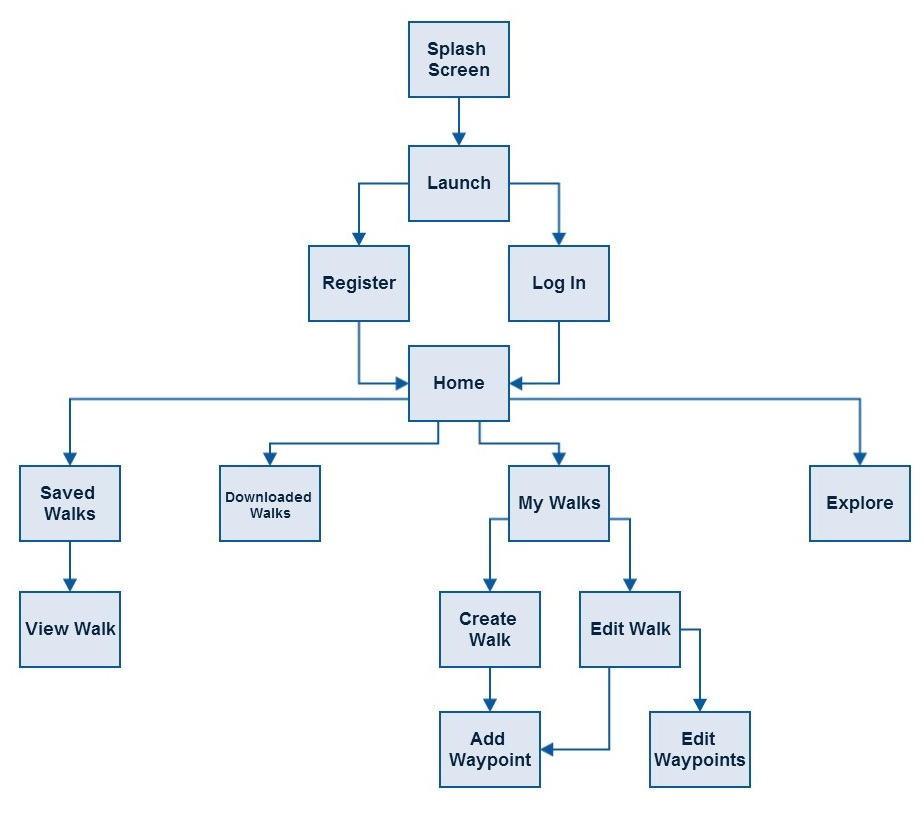
\includegraphics[width=0.8\textwidth]{chris/flow}
    \caption{Application flow diagram}
    \label{fig:flow}
\end{figure}

\subsection{Implementation}
This section details the implementation of the Android Application. Table~\ref{tab:androidsystems} lists each subsystem within the application and outlines their purpose, this is expanded upon in sections~\ref{sec:accounts} -~\ref{sec:walkexplore}. Definitions for terms used can be seen in Table~\ref{tab:androidDefs}.

\begin{longtable}{|p{2cm}|p{8cm}|}
\hline \caption{Android Definitions} \label{tab:androidDefs} \endlastfoot
\end{longtable}

\begin{longtable}{|p{5cm}|p{10cm}|}
\hline \caption{Subsystem Responsibilities - Continued on Next Page} \endfoot
\hline \caption{Subsystem Responsibilities} \label{tab:androidsystems} \endlastfoot
\hline
\textbf{Subsystem} & \textbf{Responsibility} \\ \hline
Account Authenticator & The account authenticator is responsible for communicating with the White Rock server to create, edit and authenticate accounts. Once logged in a user is able to create their own walks to share with other users, or edit those which they have previously created. \\ \hline
Database & The heart of the application, the database subsystem uses an SQLite database with a Content Provider. It is responsible for the CRUD (Create, Read, Update, Delete) operations over the data, communicating the changes in the data to the synchronisation system and presents an outward facing contract for other applications to use.  \\ \hline
Synchronisation & Responsible for sharing data between the application and the White Rock server. It receives notifications from the Database subsystem informing it when to synchronise and it receives account information from the Account Authenticator to define the permissions available for the current user's data. \\ \hline
Walk Maintenance & A series of interfaces which interface with the Database and Synchronisation subsystems to manage user created walks which can be used locally and shared with other users. \\ \hline
Walk Exploration & A Google Maps implementation which allows the user to go on a walk, following the on-screen hints. It must communicate with the Database subsystem to read and display the correct data for the chosen walk. \\ \hline
\end{longtable}

\subsubsection{Account Authenticator Subsystem}
\label{sec:accounts}

The Account Authenticator system is composed of the classes found in Table~\ref{tab:accountauth}. 

\begin{longtable}{|p{7cm}|p{10cm}|}
\hline \caption{Account Authenticator Classes - Cont. on Next Page} \endfoot
\hline \caption{Account Authenticator Classes} \label{tab:accountauth} \endlastfoot
\hline
\textbf{Class} & \textbf{Purpose} \\ \hline
AccountAuthenticator & Communicates with the native Android Account Manager to complete all operations possible for a White Rock account. These operations include getting the auth-token, presenting the log-in screen and handling authentication with the server. \\ \hline
AccountGeneral & A class which contains static variables for easy access in other classes. \\ \hline
AuthenticatorActivity & The Activity which allows a user to log in to an existing, it communicates with the Account Manager and DigitalTrailsComServerAuthenticate classes to achieve this. This is the class which has direct interaction with the user. \\ \hline
DigitalTrailsComServerAuthenticate & Communicates with the White Rock API to create user accounts and receive authentication tokens for the current user. Achieved via HTTP calls.  \\ \hline
ServerAuthentciate & An interface to be implemented by the DigitalTrailsComServerAuthenticate class, details the possible actions an account may take. \\ \hline
SignUpActivity & Similar to the AuthenticatorActivity, this class is responsible for signing a new user up to the White Rock service. \\ \hline
WhiteRockAuthenticatorService & An Android service which allow for communication with the authenticator. Extending the AbstractAccountAuthenticator class in the AccountAuthenticator method allows for the service to be connected to via an IBinder.  \\ \hline
\end{longtable}

\paragraph*{Design Justification}\mbox{}\\ 
The alternative to an Account Manager based authentication system would be to post the log in information manually to the server and return an auth token. Whilst this seems simpler on the outside, the reality is that a number of extra features, which deal with the vast majority of corner cases, are already implemented by the Account Manager. It allows the system to be aware of a user's passwords changing on other clients, dealing with expired auth tokens and provides the user with a convenient ``auto log in'' feature, much like Google's applications provide. An Account Authenticator is also necessary to implement a SyncAdapter, whilst a stub authenticator is usable this solution provides the potential for future enhancements. The application's account settings may also be found within the Android device's settings.

Figure~\ref{fig:authenticator} demonstrates how the process of retrieving an auth token works for the AccountAuthenticator. The White Rock server's authentication protocol implementation can be seen at Section~\ref{sec:authDesign}.
\begin{figure}[H]
    \centering
    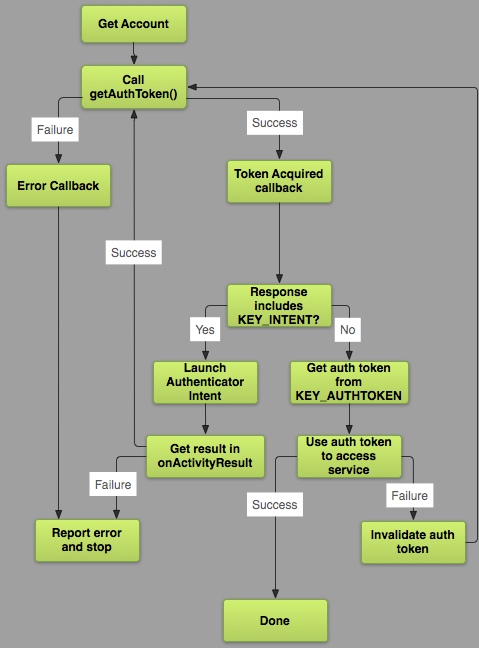
\includegraphics[width=0.8\textwidth]{authenticator}
    \caption{Authenticator Flow Diagram}
    \label{fig:authenticator}
\end{figure}

\subsubsection{Database Subsystem}
\label{sec:database}
The Database component is composed of the classes outlined in Table~\ref{tab:database}

\begin{longtable}{|p{5cm}|p{10cm}|}
\hline \caption{Database Subsystem Classes - Cont. on Next Page} \endfoot
\hline \caption{Database Subsystem Classes} \label{tab:database} \endlastfoot
\hline
\textbf{Class} & \textbf{Responsibility} \\ \hline
DatabseHandler & Responsible for checking the database exists, creating it if it does not, and providing the ContentProvider with access to the correct file. \\ \hline
WhiteRockContentProvider & Allows for the relevant CRUD operations to be performed across the tables and views defined in WhiteRockContract. It communicates with the DatabaseHandler to complete these operations. The class is accessed locally via the getContentResolver() method.  \\ \hline
WhiteRockContract & Defines the tables and views which can be operated upon via the ContentProvider. It is a public contract with clients trying to access data. It can be thought of as a public API. Since clients cannot join tables via the ContentProvider, plausible joins are also offered as well as the tables in the database. \\ \hline
DbSchema & Defines the constants for the database, including table names and the SQL to construct the database. \\ \hline
DataSource & The base class for the DataSources, a DataSource object is responsible for CRUD operations for their respective components (Walk, Waypoint, etc.) within the application, via the ContentProvider. See the attached digital Doxygen Documentation for a full list of these classes.  \\ \hline
\end{longtable}

\paragraph*{Design Justification}\mbox{}\\ 
Similar to the Account Authenticator, the benefits of the Database implementation are not necessarily obvious at first. Whilst it would have been possible to use an SQLite database without a ContentProvider, which would have been a faster implementation in the short term, this solution allows for the application to be responsive to changes in the database; provides a strict set of rules for other developers to use in the future - via the contract; allows other applications to access the database, giving the potential for supporting applications to be created; Android manages the creation and destruction of the provider, ensuring that user's data is not lost and the ContentProvider can be shut down as necessary; finally a stub, at least, is required for the implementation of a SyncAdapter, therefore implementing it fully allows for a more complete set of features.

\subsubsection{Synchronisation Subsystem}
\label{sec:synch}

The Synchronisation Subsystem consists of the classes detailed in Table~\ref{tab:sync}.

\begin{longtable}{|p{5cm}|p{10cm}|}
\hline \caption{Synchronisation Subsystem - Cont. on Next Page} \endfoot
\hline \caption{Synchronisation Subsystem} \label{tab:sync} \endlastfoot
\hline
\textbf{Class} & \textbf{Responsibility} \\ \hline
WhiteRockServerAccessor & Accesses the White Rock Server to retrieve data from, and send data to, the remote database. \\ \hline
WhiteRockSyncAdapter & Performs a threaded synchronisation with the server using the operations in the WhiteRockServerAccessor.  \\ \hline
WhiteRockSyncService & Android Service which instantiates the SyncAdapter upon creation.  \\ \hline
HTTP & \\ \hline
\end{longtable}

\paragraph*{Design Justification}\mbox{}\\ 
As is evident from the sections on the Account Authenticator (see section~\ref{sec:accounts}) and the Database Subsystem (see section~\ref{sec:database}), the SyncAdapter has been the primary cause of decisions made. 

The alternative to a SyncAdapter would be to write a Service or ServiceIntent to do the intended task, but, like the Account Authenticator, multiple benefits are provided which would be incredibly demanding on the developers to implement.

The benefits of the SyncAdapter are that it can handle background syncs between the device and the White Rock server. The adapter is registered with the platform's Sync Manager, which takes charge of triggering the SyncAdapter as needed, scheduled or requested. It manages this in a fashion which is:
\begin{description}
\item[Battery Efficient] - The system will schedule a sync when other syncs are running, or another network request has been made. This approach ensures that the device is not awoken for a single sync.
\item[Interface] - The sync adapter can be accessed from the device's Settings screen, attached to the Account created by the Account Authenticator subsystem, allowing the user to modify sync settings as they desire, or disable synchronisation automatically.
\item[Content Awareness] - Using the ContentProvider to manage the database ensures that the SyncAdapter can monitor any changes made to the data, ensuring it only performs a sync when there has been changes made to the data.
\item[Retry Mechanism] - The Sync Manager has the ability to retry any failed syncs.
\end{description}
All of these features come at no extra cost, other than the time required to understand how to write the SyncAdapter. This has been a poorly documented feature until recently.

\subsubsection{Walk Management}
\label{sec:walkcreate}

The walk management subsystem consists of the classes outlined in Table~\ref{tab:walkcreate}.

\begin{longtable}{|p{5cm}|p{10cm}|}
\hline \caption{Walk Management Subsystem - Cont. on Next Page.} \endfoot
\hline \caption{Walk Management Subsystem} \label{tab:walkcreate} \endlastfoot
\hline
\textbf{Class} & \textbf{Responsibility} \\ \hline
MyWalksActivity & The activity which allows the user to modify their created walks. Operations include creating a walk, updating a walk and deleting a walk. Initially it presents the user with the interfaces attached to MyWalkListFragment and MyWalkDetailsFragment. \\ \hline
CreateWalkFragment & The fragment which presents the user with an interface to create a new walk. \\ \hline
AddWaypointMapFragment & The GoogleMap Fragment which allows a user to add waypoints to a newly created walk. \\ \hline
AddWaypointDialogFragment & The DialogFragment which allows the user to modify details such as the waypoint's title and description. \\ \hline
EditWalkFragment & Allows the user to edit an existing walk. \\ \hline
EditWaypointMapFragment & The GoogleMap Fragment which allows a user to edit the details of current waypoints, and add new ones, to an existing walk. \\ \hline
\end{longtable}

\paragraph*{Design Justification}\mbox{}\\ 
The use of a single Activity for each aspect of the application (Register / Login, Walk Management, Walk Exploration, Walk Downloads) is a design choice which helps to keep all the relevant operations tied to a single class, the Activity. There are also performance benefits to using a single Activity with multiple, interchangeable, Fragment objects.

\subsubsection{Walk Exploration}
\label{sec:walkexplore}
A walk can be ``explored'' by a user, this implies they are going to the start location of the walk and following the waypoints. The classes for this subsystem can be seen in Table~\ref{tab:walkexplore}.

\begin{longtable}{|p{5cm}|p{10cm}|}
\hline \caption{Walk Exploration Subsystem - Cont. on Next Page.} \endfoot
\hline \caption{Walk Exploration Subsystem} \label{tab:walkexplore} \endlastfoot
\hline
\textbf{Class} & \textbf{Responsibility} \\ \hline
ChooseWalkActivity & The Activity responsible for letting a user begin a walk. It also allows the user to delete a downloaded walk from the database. Initially presents the user with the two fragments WalkDetailsFragment and WalkListFragment. \\ \hline
WalkDetailsFragment & Shows the details of the currently selected walk. \\ \hline
WalkListFragment & Allows the user to select the walk they would like to see the details of. \\ \hline
MapActivity & An Activity which contains a GoogleMap. This Activity allows the user to begin the walk, visit waypoints and view information at each one. A LocationListener and Geofences are used to keep track of the user's current location and present the relevant information as they progress. \\ \hline
\end{longtable}

\paragraph*{Design Justification}\mbox{}\\ 
All screens which allow the user to interact with a walk in some fashion, whether is starting the walk, managing walks or downloading new walks from the White Rock server use the same design. A WalkListFragment and a WalkDetailsFragment are fragments within the main Activity, in this case the ChooseWalkActivity. 

This area of the application breaks the paradigm of ``one activity for one feature'' for areas of user interaction, reimplementing multiple features of a MapFragment in the MapActivity class. The justification for this, usually poor, practice is in the added complexity of the MapActivity class as it implements Geofences, to be aware of when the user enters and exits the zone of a waypoint and the additional computational power necessary to function.

\subsubsection{Utility Classes}
There are a number of classes which are not directly linked to a subsystem but provided utility throughout the application, these classes range from custom Loaders and LoaderAdapters to container classes for the components of the system. These classes are outlined in Table~\ref{tab:utilityClasses}.

\begin{longtable}{|p{5cm}|p{10cm}|}
\hline \caption{Utility Classes - Cont. on Next Page} \endfoot
\hline \caption{Utility Classes} \label{tab:utilityClasses} \endlastfoot 
\hline
\textbf{Class} & \textbf{Responsibility} \\ \hline
WalkLoader & An AsyncTaskLoader which retrieves the List of all available Walk objects from the database, using the LoaderManager. It is used in the SearchActivity. \\ \hline
WalkLoaderAdapter & An ArrayAdapter which places elements into a custom ListFragment layout. It receives data from the WalkLoader in SearchActivity. \\ \hline
WhiteRockApp & A singleton class to retrieve the instance of the application. Used to get the Context of the application in non-Android classes. \\ \hline
Component Classes & The set of classes inside the ``uk.ac.swan.digitaltrails.components'' package, these are responsible for containing the data necessary for a single entry in each table in the database. When retrieving data from the server, JSON results are converted into the corresponding classes. \\ \hline 
\end{longtable}

\section{API} 
\label{sec:api-design}

The API is the crucial link between the Website, Application and Database. It was not originally specified but plays a key part in the eco-system of the system. It was important that the correct design and technology was selected to make that link as seamless and effective as possible. It was also important that the API was well designed and easy to use to allow for future extensions to the eco-system. 

\subsection{Technology Choices}
\label{sec:api:techChoices}

There are several important technologies which the API is built upon. The most important ones are listed below with a brief description of their function and the reasoning for choosing them. 

\begin{description}
\item[Paris] - Paris is an ORM (Object Relation Mapper) which provided a layer of abstraction between the database and the API. Rather than writing SQL queries to retrieve an object it makes it possible to use model objects to and methods to retrieve the objects.  
\item[Slim Framework] - The slim framework was chosen as the underlying framework of the API. Slim provides many low-level function which are critical to the production of a reliable API in a small and efficient package. Before it was settled on an alternative framework called Phalcon was trailed, but it proved to be overly complex and overwhelming compared to the relative simplicity of Slim. 
\item[PHP] - This is the language on which Slim runs. It is a popular free and open source web programming language. It has great support and is widely used through the world. Alternatives included C\#.NET which is a closed source and closed platform product from Microsoft. Due to the licensing fees and extra costs involved PHP quickly came to light as the best choice. 
\item[Apache] - This is the web server which handles request and responses for the API. It receives requests and passes them on to the PHP runtime for the API. Apache is the best known and most widely used web server in the world. The alternatives were Nginx and IIS. IIS is limited to Microsoft's platforms and Nginx, while well respected, is still an emerging presence in the market. 
\item[Linux] - Linux is the operating system which powers the API server. Linux is free and open source and is the most popular platform for operating a server.
\item[JSON] - JavaScript Object Notation (JSON) is a media format which is used to represent JavaScript objects as plain text. It can be used to represent far more than just JavaScript objects however. 
\end{description}

\subsection{Possible Designs}
\label{sec:api:rejected-designs} %Phalcon Framework. SOAP API's.
When work started on the API the first decision that needed to be made was on the protocol for the API. There are several popular API protocols including;

\begin{itemize}
\item SOAP
\item REST
\item JSON-RPC 
\item XML-RPC \ldots
\end{itemize}

The most popular two are SOAP and REST. SOAP was originally defined as `Simple Object Access Protocol' and is the successor to XML-RPC (XML Remote Procedure Call). It uses a XML document for its message which is sent over either the HTTP or SMTP application protocols. The XML document which is transmitted with a SOAP request has several parts. The document will start with an `Envelope' which contains all of the data. Inside the `Envelope' there is an optional `Header', a compulsory `Body' which contains request data, and an optional `Fault' which contains any errors which have occurred. Listing \ref{lst:soap} shows an example of a SOAP request.

\lstset{language=xml,
keywordstyle=\color{Maroon},
commentstyle=\color{OliveGreen},
showstringspaces=false, tabsize=4, breaklines=true, showspaces=false, stringstyle=\color{Blue}}

\begin{lstlisting}[captionpos=b, caption=An example SOAP request., label=lst:soap, frame=single]
POST /InStock HTTP/1.1
Host: www.example.org
Content-Type: application/soap+xml; charset=utf-8
Content-Length: 299
SOAPAction: "http://www.w3.org/203/05/soap-envelope"
 
<?xml version="1.0"?>
<soap:Envelope xmlns:soap="http://www.w3.org/203/05/soap-envelope">
  <soap:Header>
  </soap:Header>
  <soap:Body>
    <m:GetStockPrice xmlns:m="http://www.example.org/stock">
      <m:StockName>IBM</m:StockName>
    </m:GetStockPrice>
  </soap:Body>
</soap:Envelope>
\end{lstlisting}

REST, on the other hand, is a stateless system which communicates via URI's, any media (such as JSON or XML) and HTTP Methods. REST stands for Representational State Transfer, which implies a representation of the current state must be transferred to the API with reach request. A REST request to retrieve an object can be as simple as \lstinline$GET http:\\example.com\api\users$. The simplicity of REST lends its self to many situations and makes it easy to adapt to specific cases. 

\subsection{Chosen Design}
For the API it was decided to harness the REST protocol. The decision was made after analysing both SOAP and REST and the advantages and disadvantages of both. In the end the overly verbose nature of SOAP led to the decision of a REST api.  The ability to use JSON with REST requests was also a deciding factor as this greatly reduced the workload when communicating with the API from JavaScript. This helped us design a modern and intuitive API with a clear structure and flow. 

\subsection{Classes}
\label{sec:api:class}
The API has several `Model' classes to represent the Database tables and the objects that are stored within them. The objects are related through the database and can retrieve the related models through method calls. The relations between the models is shown in Figure \ref{fig:datamodels}, where every model is a possible entry point. Using these models it is possible to, for example, use an `English Walk Description' to return all related 'Waypoint Images'. 

\begin{figure}[H]
    \centering
    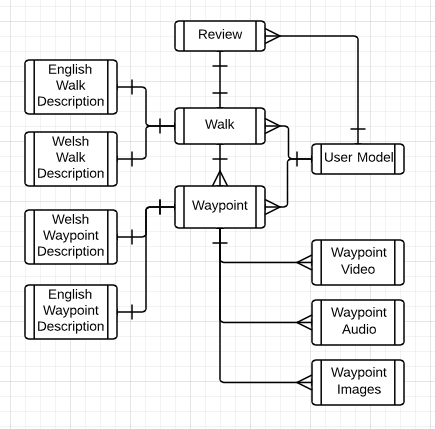
\includegraphics[width=0.5\textwidth]{DataModels}
    \caption{The Data Model and their relations.}
    \label{fig:datamodels}
\end{figure}

The API has several main object collections, which are `Walks', `Waypoints', `Users', `Waypoint Images', `Waypoint Audio', `Waypoint Video', `Walk Reviews' and `Sessions'. Each collection has a specific route in the API which maps to a collection controller. When a route is called a method in the relavent controller is called. The method is passed a variable called \$app. This contains the requests and response objects. When the controller has completed its work it writes the response to the \$app object and returns to the index file which initially handled the request. If there is no more work to be done the \$app object sends the response. 

\begin{figure}[H]
    \centering
    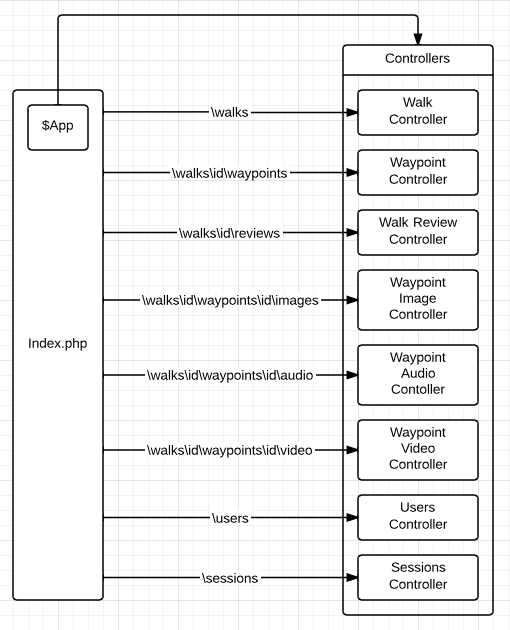
\includegraphics[width=0.5\textwidth]{ControllerRoutes}
    \caption{The connection between routes and controllers.}
    \label{fig:controllerroutes}
\end{figure}

Each controller has methods to respond to different requests, a generic controller will have `getOne', `getAll', `add', `update', `remove' and `search'. The methods match up to specific routes. For example `getOne' normally matches to \textbf{GET} \url{/resources/id} and `add' matches \textbf{POST} \url{/resources}. 

\subsubsection{Walk Controller}

The walk controller process request for several different functions. It provides the most functionality allowing not just for traditional CRUD operations but also for searching. All methods return a JSON \emph{Walk} object, except for \lstinline$getAll()$ which returns an array of \emph{Walk} objects. \textbf{POST} and \textbf{PUT} requests expect a JSON \emph{Walk} object to be passed in the request body. 

\begin{table}[H]
\centering
\begin{tabular}{l | l | l}
HTTP Method & Route & Controller Method\\ \hline
\textbf{\textcolor{Maroon}{GET}} & \url{/walks} & \lstinline$getAll()$ \\
\textbf{\textcolor{Maroon}{GET}} & \url{/walks/}\bfurl{id} & \lstinline$getOne(id)$\\
\textbf{\textcolor{Maroon}{POST}} & \url{/walks} & \lstinline$add()$\\
\textbf{\textcolor{Maroon}{PUT}} & \url{/walks/}\bfurl{id} & \lstinline$update(id)$\\
\textbf{\textcolor{Maroon}{DELETE}} & \url{/walks/}\bfurl{id} & \lstinline$delete(id)$\\
\textbf{\textcolor{Maroon}{GET}} & \url{/walks/search/}\bfurl{query} & \lstinline$search(query)$\\
\end{tabular}
\caption{Routes and Methods in the Walks Controller}
\label{tab:walksController}
\end{table}

\subsubsection{Waypoint Controller}

The waypoint controller provides the basic CRUD operations. When adding or getting all waypoints it requires the id of the walk they should belong to. When acting upon an individual waypoint it needs the waypoints id, called \bfurl{wid} in the table. All methods return a JSON \emph{Waypoint} object, except for \lstinline$getAll()$ which returns an array of \emph{Waypoint} objects. \textbf{POST} and \textbf{PUT} requests expect a JSON \emph{Waypoint} object to be passed in the request body. 

\begin{table}[H]
\centering
\begin{tabular}{l | l | l}
HTTP Method & Route & Controller Method\\ \hline
\textbf{\textcolor{Maroon}{GET}} & \url{/walks/}\bfurl{id}\url{/waypoints} & \lstinline$getAll(id)$ \\
\textbf{\textcolor{Maroon}{GET}} & \url{/walks/}\bfurl{id}\url{/waypoints/}\bfurl{wid} & \lstinline$getOne(wid)$\\
\textbf{\textcolor{Maroon}{POST}} & \url{/walks/}\bfurl{id}\url{/waypoints} & \lstinline$add(id)$\\
\textbf{\textcolor{Maroon}{PUT}} & \url{/walks/}\bfurl{id}\url{/waypoints/}\bfurl{wid} & \lstinline$update(wid)$\\
\textbf{\textcolor{Maroon}{DELETE}} & \url{/walks/}\bfurl{id}\url{/waypoints/}\bfurl{wid} & \lstinline$delete(wid)$\\
\end{tabular}
\caption{Routes and Methods in the Waypoint Controller}
\label{tab:waypointController}
\end{table}

\subsubsection{Walk Review Controller}

The walk review controller allows the user to get all reviews for a walk, get an individual review, add a review to a walk and delete a review. Users are prohibited from updating a review once it has been submitted. Users are expected to pass a valid walk object in JSON when they add and will receive back valid objects with every request.  All methods return a JSON \emph{Review} object, except for \lstinline$getAll()$ which returns an array of \emph{Review} objects. \textbf{POST} requests expect a JSON \emph{Review} object to be passed in the request body. 

\begin{table}[H]
\centering
\begin{tabular}{l | l | l}
HTTP Method & Route & Controller Method\\ \hline
\textbf{\textcolor{Maroon}{GET}} & \url{/walks/}\bfurl{id}\url{/reviews} & \lstinline$getAll(id)$ \\
\textbf{\textcolor{Maroon}{GET}} & \url{/walks/}\bfurl{id}\url{/reviews/}\bfurl{rid} & \lstinline$getOne(rid)$\\
\textbf{\textcolor{Maroon}{POST}} & \url{/walks/}\bfurl{id}\url{/reviews} & \lstinline$add(id)$\\
\textbf{\textcolor{Maroon}{DELETE}} & \url{/walks/}\bfurl{id}\url{/reviews/}\bfurl{rid} & \lstinline$delete(rid)$\\
\end{tabular}
\caption{Routes and Methods in the Walk Review Controller}
\label{tab:waypointController}
\end{table}

\subsubsection{Waypoint Image Controller}

Waypoint Image Controller allows users to upload images for waypoints. Users are able to add, remove and get images (either all of them or just one). When uploading a file the request should contain the file, which is then moved within the server and stored and a thumbnail is generated. All methods return a JSON \emph{Image} object, except for \lstinline$getAll()$ which returns an array of \emph{Image} objects. \textbf{POST} requests expect a JSON \emph{Image} object and an image file to be passed in the request body. Only JPEG, GIF and PNG images are accepted. 

\begin{table}[H]
\centering
\begin{tabular}{l | l | l}
HTTP Method & Route & Controller Method\\ \hline
\textbf{\textcolor{Maroon}{GET}} & \url{/walks/}\bfurl{id}\url{/waypoints/}\bfurl{wid}\url{/images} & \lstinline$getAll(wid)$ \\
\textbf{\textcolor{Maroon}{GET}} & \url{/walks/}\bfurl{id}\url{/waypoints/}\bfurl{wid}\url{/images/}\bfurl{img_id} & \lstinline$getOne(img_id)$\\
\textbf{\textcolor{Maroon}{POST}} & \url{/walks/}\bfurl{id}\url{/waypoints/}\bfurl{wid}\url{/images} & \lstinline$add(wid)$\\
\textbf{\textcolor{Maroon}{DELETE}} & \url{/walks/}\bfurl{id}\url{/waypoints/}\bfurl{wid}\url{/images/}\bfurl{img_id} & \lstinline$delete(wid)$\\
\end{tabular}
\caption{Routes and Methods in the Waypoint Image Controller}
\label{tab:waypointImageController}
\end{table}

\subsubsection{Waypoint Audio Controller}

Waypoint Audio Controller is similar to the image controller, it allows users to upload audio for waypoints. Users are able to add, remove and get audio samples (either all of them or just one). When uploading a file the request should contain the file, which is then moved within the server and stored. All methods return a JSON \emph{Audio} object, except for \lstinline$getAll()$ which returns an array of \emph{Audio} objects. \textbf{POST}requests expect a JSON \emph{Audio} object and a sound file to be passed in the request body. 

\begin{table}[H]
\centering
\begin{tabular}{l | l | l}
HTTP Method & Route & Controller Method\\ \hline
\textbf{\textcolor{Maroon}{GET}} & \url{/walks/}\bfurl{id}\url{/waypoints/}\bfurl{wid}\url{/images} & \lstinline$getAll(wid)$ \\
\textbf{\textcolor{Maroon}{GET}} & \url{/walks/}\bfurl{id}\url{/waypoints/}\bfurl{wid}\url{/images/}\bfurl{img_id} & \lstinline$getOne(img_id)$\\
\textbf{\textcolor{Maroon}{POST}} & \url{/walks/}\bfurl{id}\url{/waypoints/}\bfurl{wid}\url{/images} & \lstinline$add(wid)$\\
\textbf{\textcolor{Maroon}{DELETE}} & \url{/walks/}\bfurl{id}\url{/waypoints/}\bfurl{wid}\url{/images/}\bfurl{img_id} & \lstinline$delete(wid)$\\
\end{tabular}
\caption{Routes and Methods in the Waypoint Audio Controller}
\label{tab:waypointAudioController}
\end{table}

\subsubsection{Waypoint Video Controller}

Waypoint Video Controller is very similar to the image controller. Users are able to add, remove and get videos (either all of them or just one). When uploading a file the request should contain the file, which is then moved within the server and stored and a thumbnail is generated. All methods return a JSON \emph{Video} object, except for \lstinline$getAll()$ which returns an array of \emph{Video} objects. \textbf{POST} requests expect a JSON \emph{Video} object and a video file to be passed in the request body. 

\begin{table}[H]
\centering
\begin{tabular}{l | l | l}
HTTP Method & Route & Controller Method\\ \hline
\textbf{\textcolor{Maroon}{GET}} & \url{/walks/}\bfurl{id}\url{/waypoints/}\bfurl{wid}\url{/images} & \lstinline$getAll(wid)$ \\
\textbf{\textcolor{Maroon}{GET}} & \url{/walks/}\bfurl{id}\url{/waypoints/}\bfurl{wid}\url{/images/}\bfurl{img_id} & \lstinline$getOne(img_id)$\\
\textbf{\textcolor{Maroon}{POST}} & \url{/walks/}\bfurl{id}\url{/waypoints/}\bfurl{wid}\url{/images} & \lstinline$add(wid)$\\
\textbf{\textcolor{Maroon}{DELETE}} & \url{/walks/}\bfurl{id}\url{/waypoints/}\bfurl{wid}\url{/images/}\bfurl{img_id} & \lstinline$delete(wid)$\\
\end{tabular}
\caption{Routes and Methods in the Waypoint Video Controller}
\label{tab:waypointVideoController}
\end{table}

\subsubsection{User Controller}

The User Controller allows users to get users (Either all or just one), allows user to be added (Registration), allows users to be searched for and lets uses update or delete their own account. If a user tries to modify or delete an account that is no their own the controller will block the request and return a 403 Forbidden error. All methods return a JSON \emph{User} object, except for \lstinline$getAll()$ which returns an array of \emph{User} objects. \textbf{POST} and \textbf{PUT} requests expect a JSON \emph{User} object to be passed in the request body. 

\begin{table}[H]
\centering
\begin{tabular}{l | l | l}
HTTP Method & Route & Controller Method\\ \hline
\textbf{\textcolor{Maroon}{GET}} & \url{/users} & \lstinline$getAll()$ \\
\textbf{\textcolor{Maroon}{GET}} & \url{/users/}\bfurl{id} & \lstinline$getOne(id)$\\
\textbf{\textcolor{Maroon}{POST}} & \url{/users} & \lstinline$add()$\\
\textbf{\textcolor{Maroon}{PUT}} & \url{/users/}\bfurl{id} & \lstinline$update(id)$\\
\textbf{\textcolor{Maroon}{DELETE}} & \url{/users/}\bfurl{id} & \lstinline$delete(id)$\\
\textbf{\textcolor{Maroon}{GET}} & \url{/users/search/}\bfurl{query} & \lstinline$search(query)$\\
\end{tabular}
\caption{Routes and Methods in the User Controller}
\label{tab:usersController}
\end{table}

\subsubsection{Session Controller}

The session controller provides only two features, login and logout. Login will assign the user an authorisation token to authenticate their requests and logout will remove that auth token from the user. Login expects a JSON \emph{User} object with username and password set. It will then return a \emph{User} object with an authToken rather than the password. 

\begin{table}[H]
\centering
\begin{tabular}{l | l | l}
HTTP Method & Route & Controller Method\\ \hline
\textbf{\textcolor{Maroon}{POST}} & \url{/sessions} & \lstinline$login()$\\
\textbf{\textcolor{Maroon}{DELETE}} & \url{/sessions} & \lstinline$logout()$\\
\end{tabular}
\caption{Routes and Methods in the Session}
\label{tab:SessionController}
\end{table}


\section{The Database}
\label{sec:database-design}

\begin{figure}[H]
    \centering
    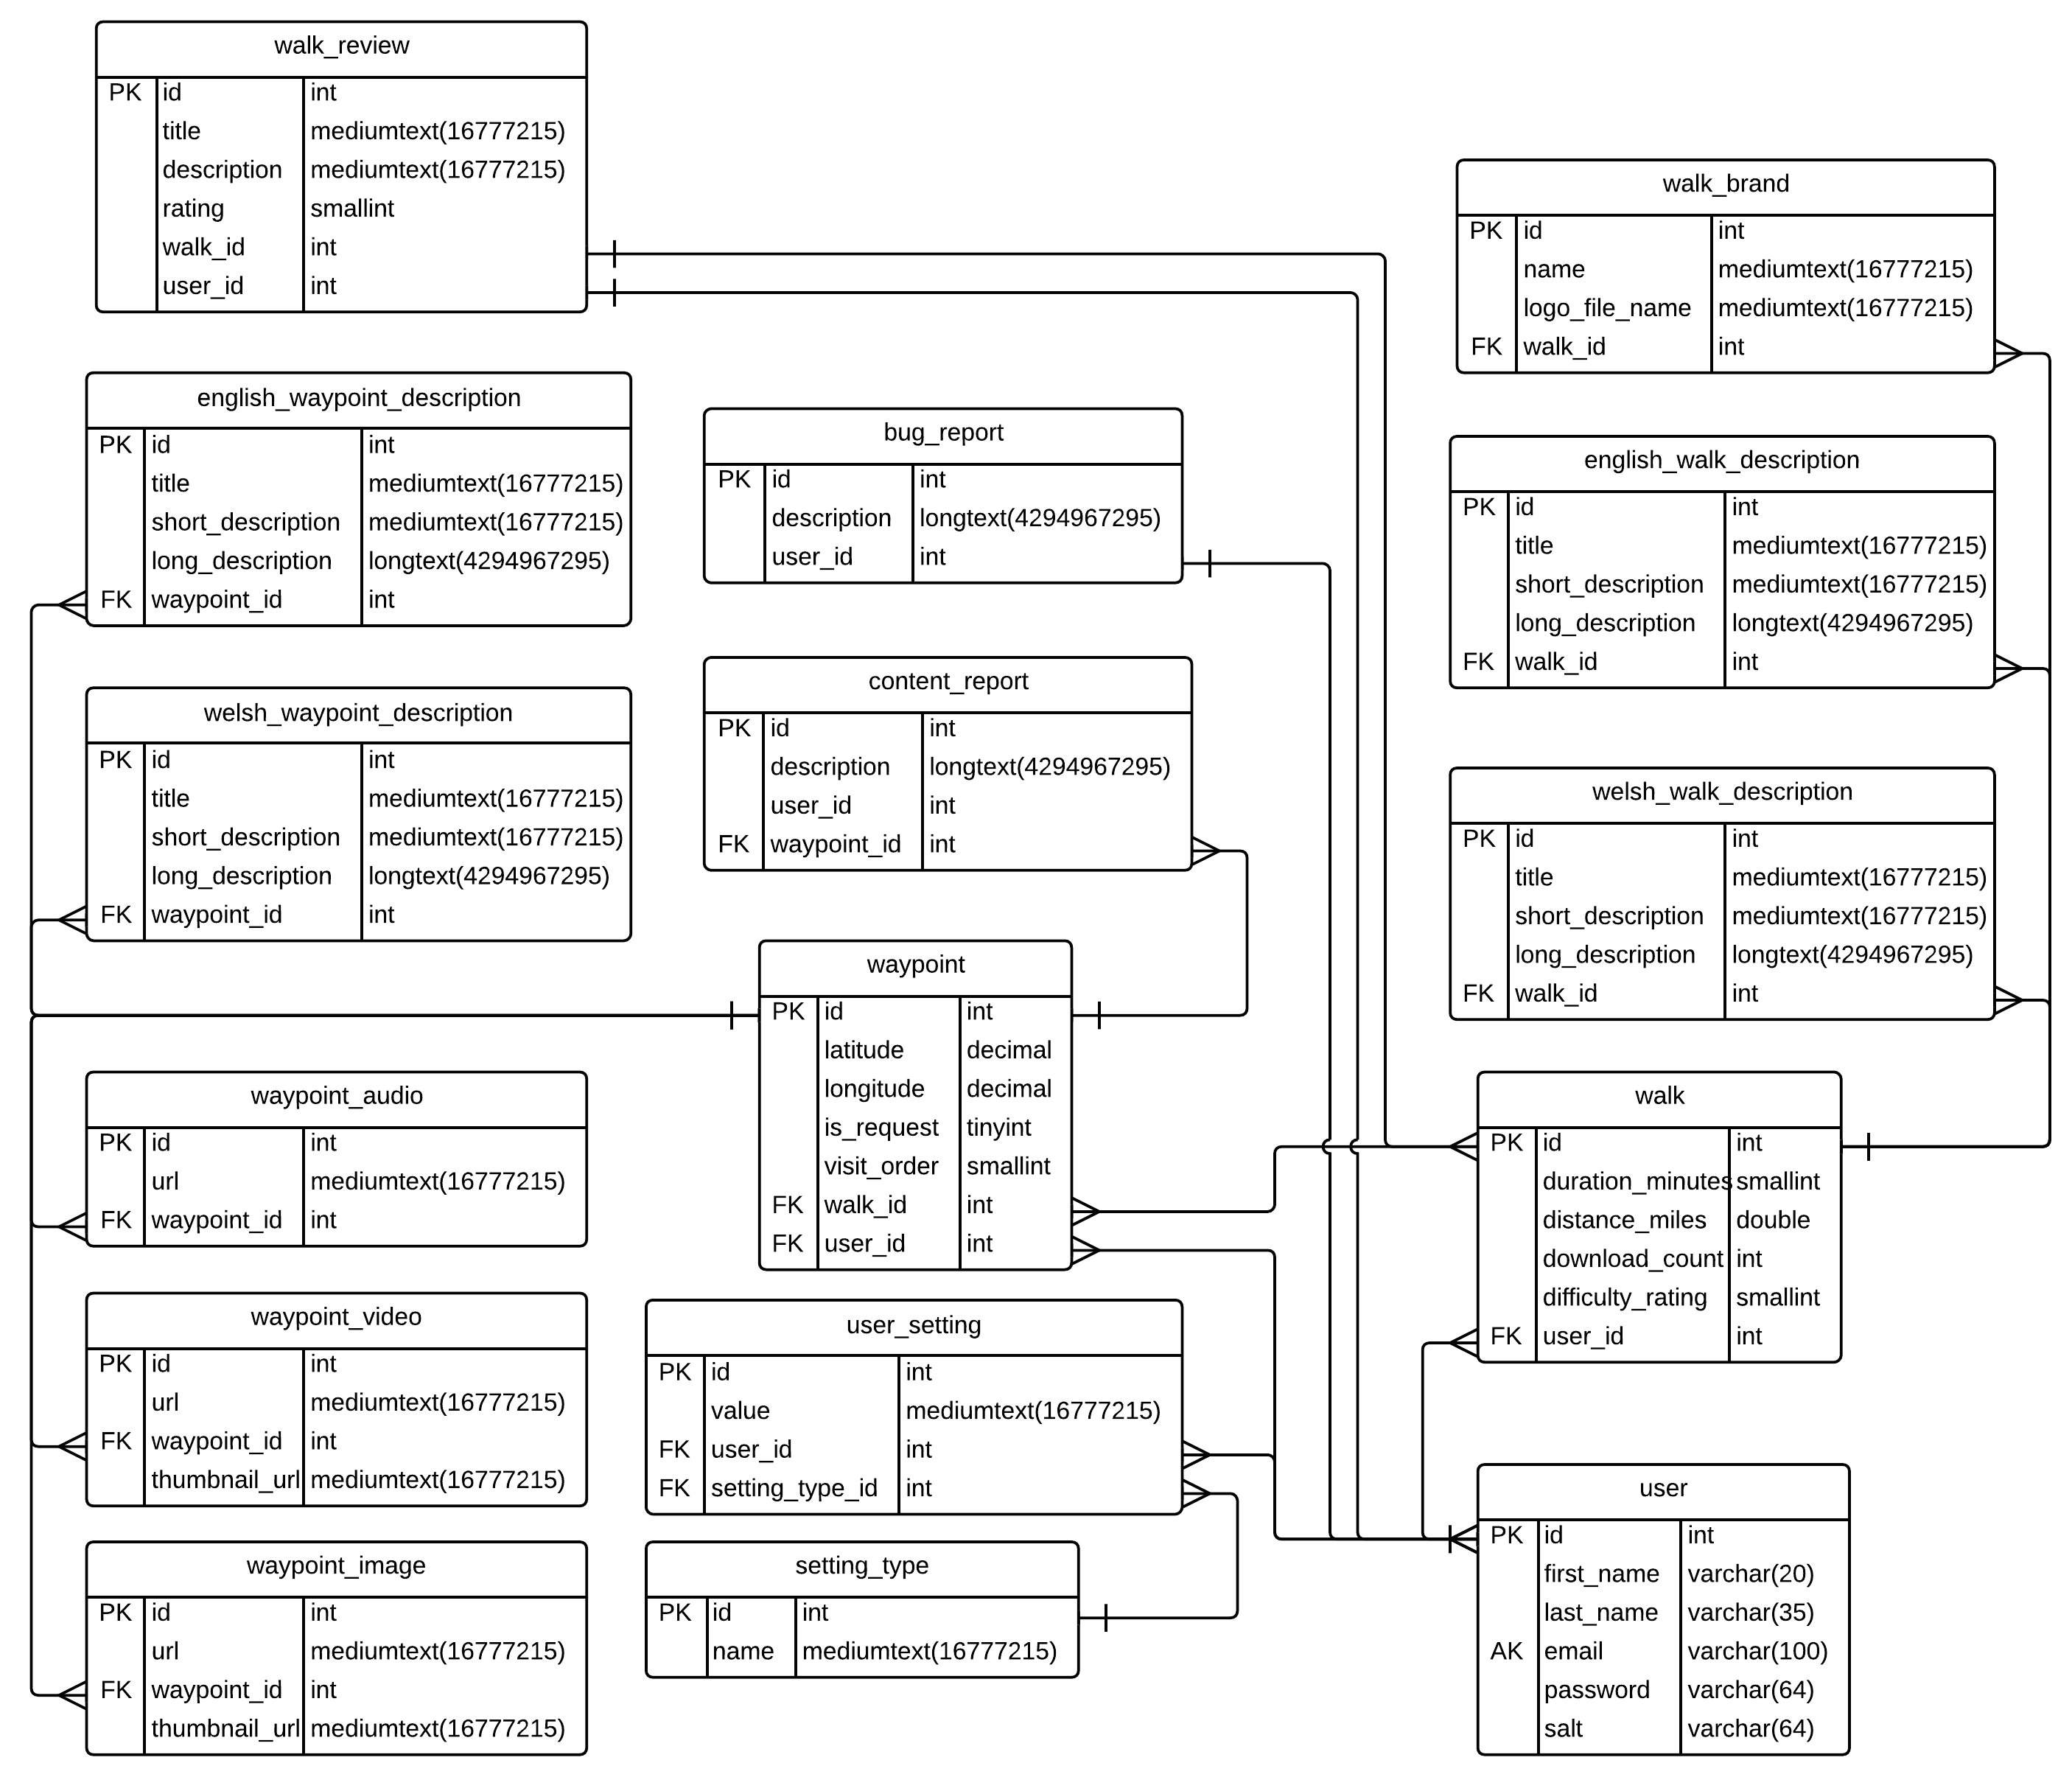
\includegraphics[width=\textwidth]{ERGroup}
    \caption{The Database Schema}
    \label{fig:databaseschema}
\end{figure}

The database is shown in Figure \ref{fig:databaseschema}. It was designed in 3rd Normal Form to reduce data duplication and ensure that integrity through keys. Tables are related by their primary key, called id. If a table is dependent on another table it can use a foreign key column which references the primary key of the secondary table. This design was chosen because it allows for the expansion of the database and it ensures the integrity and stability of the data. There was the possibility of progressing the database to a higher normal form, however the work to achieve this would out weight any performance benefits and the database in 3rdNF nicely matches the structure of the API.

\subsection{Tables}

\subsubsection{walk}
The walk table holds all of the data directly related to a walk. It has a primary key \textit{id}, and a foreign key \textit{user\_id} which relates the walk to the user who owns it by the user's \textit{id} field. 

\textbf{\textcolor{Maroon}{id:}} int - Primary key - The unique ID of the row. \\
\textbf{\textcolor{Maroon}{duration\_minutes:}} smallint -  The duration of the walk to the nearest minutes.\\
\textbf{\textcolor{Maroon}{distance\_miles:}} double - The distance of the walk in miles.\\
\textbf{\textcolor{Maroon}{download\_count:}} int - A count of how many times the walk has been download to an app. \\
\textbf{\textcolor{Maroon}{difficulty\_rating:}} Integer - Foreign key - The ID of the user who uploaded the Document. \\
\textbf{\textcolor{Maroon}{user\_id:}} int - Foreign key - The ID of the user who created the walk.

\subsubsection{waypoint}
The waypoint table stores all waypoints. Each waypoint has a unique \textit{id} as its primary key, a foreign key \textit{user\_id} which links it to the creator via there own \textit{id} and a foreign key \textit{walk\_id} which relates the waypoint to a specific walk by the walks unique \textit{id} field. 

\textbf{\textcolor{Maroon}{id:}} int - Primary key - The unique ID of the row. \\
\textbf{\textcolor{Maroon}{latitude:}} decimal -  The duration of the walk to the nearest minutes.\\
\textbf{\textcolor{Maroon}{longitude:}} decimal - The distance of the walk in miles.\\
\textbf{\textcolor{Maroon}{is\_request:}} tinyint - A count of how many times the walk has been download to an app. \\
\textbf{\textcolor{Maroon}{visit\_order:}} smallint - The order the waypoint should be visited in. \\
\textbf{\textcolor{Maroon}{walk\_id:}} int - Foreign key - The ID of the walk the waypoint belongs to.\\
\textbf{\textcolor{Maroon}{user\_id:}} int - Foreign key - The ID of the user who created the waypoint.

\subsubsection{user}
The user table holds all registered users. Every user is assigned a unique \textit{id} as its primary key for relations. The `email' field is designated a `Unique Index' meaning that no two users can have the same email address. 

\textbf{\textcolor{Maroon}{id:}} int - Primary key - The unique ID of the row. \\
\textbf{\textcolor{Maroon}{first\_name:}} varchar(20) -  The first name of the user.\\
\textbf{\textcolor{Maroon}{last\_name:}} varchar(35) - The last name of the user.\\
\textbf{\textcolor{Maroon}{email:}} varchar(100) - Unique - The email address of the user. \\
\textbf{\textcolor{Maroon}{password:}} varchar(64) - The hashed password of the user. \\
\textbf{\textcolor{Maroon}{salt:}} varchar(64) - The salt used to hash the password.

\subsubsection{walk\_review}
The walk reviews table hold users reviews of a walk. As normal each review gets a unique \textit{id} as its primary key. Reviews then have foreign keys for \textit{user\_id} and \textit{walk\_id} which relate it to the correct walk and user. 

\textbf{\textcolor{Maroon}{id:}} int - Primary key - The unique ID of the row. \\
\textbf{\textcolor{Maroon}{title:}} mediumtext -  The review title.\\
\textbf{\textcolor{Maroon}{description:}} mediumtext - The reviewers description of the walk.\\
\textbf{\textcolor{Maroon}{rating:}} smallint - The rating the user gave the walk. \\
\textbf{\textcolor{Maroon}{walk\_id:}} int - Foreign key - The ID of the walk the review belongs to.\\
\textbf{\textcolor{Maroon}{user\_id:}} int - Foreign key - The ID of the user who created the review.

\subsubsection{walk\_brand}
The walk brand holds some style information for a walk. It has a primary key \textit{id} and is linked to the walk by the foreign key \textit{walk\_id}. 

\textbf{\textcolor{Maroon}{id:}} int - Primary key - The unique ID of the row. \\
\textbf{\textcolor{Maroon}{name:}} mediumtext -  The walks branding name.\\
\textbf{\textcolor{Maroon}{logo\_file\_name:}} mediumtext - The walks logo.\\
\textbf{\textcolor{Maroon}{walk\_id:}} int - Foreign key - The ID of the walk the review belongs to.\\

\subsubsection{english\_walk\_description}
The english walk description table holds the english version of the walk description. Its mapped to a particular walk through the foreign key \textit{walk\_id}. It has its own primary key \textit{id} which is unique to that english walk description. 

\textbf{\textcolor{Maroon}{id:}} int - Primary key - The unique ID of the row. \\
\textbf{\textcolor{Maroon}{title:}} mediumtext -  The walk title .\\
\textbf{\textcolor{Maroon}{short\_description:}} mediumtext - The a short description of the walk.\\
\textbf{\textcolor{Maroon}{long\_description:}} long text - The a long description of the walk. \\
\textbf{\textcolor{Maroon}{walk\_id:}} int - Foreign key - The ID of the walk the description belongs to.

\subsubsection{welsh\_walk\_description}
The welsh walk description table holds the welsh version of the walk description. Its mapped to a particular walk through the foreign key \textit{walk\_id}. It has its own primary key \textit{id} which is unique to that welsh walk description. 

\textbf{\textcolor{Maroon}{id:}} int - Primary key - The unique ID of the row. \\
\textbf{\textcolor{Maroon}{title:}} mediumtext -  The walk title.\\
\textbf{\textcolor{Maroon}{short\_description:}} mediumtext - The a short description of the walk.\\
\textbf{\textcolor{Maroon}{long\_description:}} long text - The a long description of the walk. \\
\textbf{\textcolor{Maroon}{walk\_id:}} int - Foreign key - The ID of the walk the description belongs to.

\subsubsection{english\_waypoint\_description}
The english waypoint description table holds the english version of the waypoint description. Its mapped to a particular walk through the foreign key \textit{waypoint\_id}. It has its own primary key \textit{id} which is unique to that english waypoint description. 

\textbf{\textcolor{Maroon}{id:}} int - Primary key - The unique ID of the row. \\
\textbf{\textcolor{Maroon}{title:}} mediumtext -  The waypoint title.\\
\textbf{\textcolor{Maroon}{short\_description:}} mediumtext - The a short description of the waypoint.\\
\textbf{\textcolor{Maroon}{long\_description:}} long text - The a long description of the waypoint. \\
\textbf{\textcolor{Maroon}{waypoint\_id:}} int - Foreign key - The ID of the waypoint the description belongs to.

\subsubsection{welsh\_waypoint\_description}
The welsh waypoint description table holds the welsh version of the waypoint description. Its mapped to a particular walk through the foreign key \textit{waypoint\_id}. It has its own primary key \textit{id} which is unique to that welsh waypoint description. 

\textbf{\textcolor{Maroon}{id:}} int - Primary key - The unique ID of the row. \\
\textbf{\textcolor{Maroon}{title:}} mediumtext -  The waypoint title.\\
\textbf{\textcolor{Maroon}{short\_description:}} mediumtext - The a short description of the waypoint.\\
\textbf{\textcolor{Maroon}{long\_description:}} long text - The a long description of the waypoint. \\
\textbf{\textcolor{Maroon}{waypoint\_id:}} int - Foreign key - The ID of the waypoint the description belongs to.

\subsubsection{waypoint\_audio}
The waypoint audio table holds information about audio files. They are mapped to the waypoints which they belong to via the foreign key \textit{waypoint\_id} and have their own primary key \textit{id}.

\textbf{\textcolor{Maroon}{id:}} int - Primary key - The unique ID of the row. \\
\textbf{\textcolor{Maroon}{url:}} mediumtext -  The files url.\\
\textbf{\textcolor{Maroon}{waypoint\_id:}} int - Foreign key - The ID of the waypoint the audio belongs to.

\subsubsection{waypoint\_image}
The waypoint image table holds information about image files. They are mapped to the waypoints which they belong to via the foreign key \textit{waypoint\_id} and have their own primary key \textit{id}.

\textbf{\textcolor{Maroon}{id:}} int - Primary key - The unique ID of the row. \\
\textbf{\textcolor{Maroon}{url:}} mediumtext -  The files url.\\
\textbf{\textcolor{Maroon}{thumbnail\_url:}} mediumtext - The thumbnails url.\\
\textbf{\textcolor{Maroon}{waypoint\_id:}} int - Foreign key - The ID of the waypoint the image belongs to.

\subsubsection{waypoint\_video}
The waypoint video table holds information about video files. They are mapped to the waypoints which they belong to via the foreign key \textit{waypoint\_id} and have their own primary key \textit{id}.

\textbf{\textcolor{Maroon}{id:}} int - Primary key - The unique ID of the row. \\
\textbf{\textcolor{Maroon}{url:}} mediumtext -  The files url.\\
\textbf{\textcolor{Maroon}{thumbnail\_url:}} mediumtext - The thumbnails url.\\
\textbf{\textcolor{Maroon}{waypoint\_id:}} int - Foreign key - The ID of the waypoint the video belongs to.

\subsubsection{user\_setting}
The users settings table hold the value of each setting for each user. Each row is a specific settings values mapped to a setting type by \textit{setting\_type\_id} and to the user by \textit{user\_id}. Each row has a unique id given by the primary key field \textit{id}.

\textbf{\textcolor{Maroon}{id:}} int - Primary key - The unique ID of the row. \\
\textbf{\textcolor{Maroon}{value:}} mediumtext -  The setting value.\\
\textbf{\textcolor{Maroon}{user\_id:}} int - Foreign key - The ID of the user the setting belongs to.\\
\textbf{\textcolor{Maroon}{setting\_type\_id:}} int - Foreign key - The ID of the setting type.

\subsubsection{setting\_type}
The setting type table stores all the settings a user can have. Each one has a unique \textit{id} as its primary key which is used by user\_settings to assign settings to users.

\textbf{\textcolor{Maroon}{id:}} int - Primary key - The unique ID of the row. \\
\textbf{\textcolor{Maroon}{name:}} mediumtext -  The setting name.\\

\subsubsection{content\_report}
The Content Report table stores any reports users have filed about a waypoint. The reports have a unique primary key field \textit{id} and are related to the reported waypoint via a foreign key \textit{waypoint\_id}. 

\textbf{\textcolor{Maroon}{id:}} int - Primary key - The unique ID of the row. \\
\textbf{\textcolor{Maroon}{description:}} long text -  The description of the report .\\
\textbf{\textcolor{Maroon}{user\_id:}} int - Foreign key - The ID of the user the report belongs to.\\
\textbf{\textcolor{Maroon}{waypoint\_id:}} int - Foreign key - The ID of the waypoint being reported.

\subsubsection{bug\_report}
The Bug report table is used to store bugs in the program that are reported by users. They have a unique primary key field \textit{id} and are related to the user who reported it via a foreign key \textit{user\_id}

\textbf{\textcolor{Maroon}{id:}} int - Primary key - The unique ID of the row. \\
\textbf{\textcolor{Maroon}{description:}} long text -  The description of the report .\\
\textbf{\textcolor{Maroon}{user\_id:}} int - Foreign key - The ID of the user the report belongs to.\\

\chapter{Testing}
\label{sec:testing}
\section{Unit Testing}
\label{sec:unit-testint}
\section{Acceptance Testing}
\label{sec:acceptance-testint}

\subsection{Web Portal}

\label{test:POR-T01}
\noindent\textbf{Test Code:} POR-T01\\
\textbf{Asserts Specification:} WEBSPEC1, WEBSPEC2, WEBSPEC3 \\ 
\textbf{Criteria:} \begin{itemize}
                     \item The web portal should have a `Register' button for users that are not logged in.
                     \item Clicking `Register' should display a view with `Name', `Email Address', `Password', `Password Confirmation' text fields and `Register' and `Cancel' buttons.
                     \item Clicking `Cancel' should return the user to the index page.
                     \item Clicking `Register' should create a user and log them in.
                   \end{itemize}  
\textbf{Result:} \textcolor{green}{PASS}\\ 
\textbf{Description:} This set of test cases tests that a user can register a new account with the Web Portal. It also tests that the correct fields are displayed on the form and that users are logged in after registration.\\

\label{test:POR-T02}
\noindent\textbf{Test Code:} POR-T02\\
\textbf{Asserts Specification:} WEBSPEC5, WEBSPEC6, WEBSPEC7, WEBSPEC8, WEBSPEC9, WEBSPEC10 \\ 
\textbf{Criteria:} \begin{itemize}
                     \item A `Login' button should be visible to users that are not logged in.
                     \item Clicking `Login' should present a modal dialogue with `Username' and `Password' fields and `Login' and `Cancel' buttons.
                     \item Clicking `Login' should create an authenticated session for the user and store it in a temporary cookie.
                     \item Clicking `Cancel' should dismiss the modal dialogue.
                     \item When users are logged in they should be presented with a `Logout' link.
                     \item Clicking `Logout' should delete the session cookie and return the user to the index page as a guest.
                   \end{itemize}  
\textbf{Result:} \textcolor{green}{PASS}\\ 
\textbf{Description:} This set of test cases tests that a registered user can log in to the application. It also tests that the correct fields are on the login form and that users can also log out. Finally, it tests the technical requirement of session token storage. \\

\label{test:POR-T03}
\noindent\textbf{Test Code:} POR-T03\\
\textbf{Asserts Specification:} WEBSPEC11, WEBSPEC12, WEBSPEC13, WEBSPEC14 \\ 
\textbf{Criteria:} \begin{itemize}
                     \item The web portal should feature an `Edit Account' button.
                     \item Clicking the `Edit Account' should display a view that allows the user to edit their `full name, email and password', a `Cancel' button and a `Save' button.
                     \item Clicking the `Save' button should validate the full name, email and password text boxes. If successful, a notification will inform the user that changes were made to their details.
                     \item Clicking the `Cancel' button should cancel current changes made to the user's details.
                   \end{itemize}  
\textbf{Result:} \textcolor{green}{PASS}\\ 
\textbf{Description:} This set of test cases tests that a registered user can change their account details such as their \emph{full name}, \emph{email} and \emph{password}. It also tests that the correct fields are present. \\

\label{test:POR-T04}
\noindent\textbf{Test Code:} POR-T04\\
\textbf{Asserts Specification:} WEBSPEC15, WEBSPEC16, WEBSPEC17 \\ 
\textbf{Criteria:} \begin{itemize}
                     \item All web portal views should feature the company logo and use a house colour scheme.
                     \item The `user account settings' view should feature a company branding tab, allowing the user to attach their company logo to a walk.
                     \item The company branding tab should feature a `Browse' button, allowing the user to browse their computer for a particular image and should feature a `Save' button, allowing the user to upload their image.
                   \end{itemize}  
\textbf{Result:} \textcolor{green}{PASS} - It was decided that company branding would be added to a walk using a cover image rather than tied to a specific account.\\ 
\textbf{Description:} This set of test cases tests that a registered user can change the branding of their walks using an image from their computer. The brand logo should then be visible on all the user's created walks. \\

\label{test:POR-T05}
\noindent\textbf{Test Code:} POR-T05\\
\textbf{Asserts Specification:} WEBSPEC18, WEBSPEC19, WEBSPEC20, WEBSPEC21, WEBSPEC22, WEBSPEC23, WEBSPEC24\\ 
\textbf{Criteria:} \begin{itemize}
                     \item Successfully logging in should take the user to a `Homepage' view featuring their own walks and contributions.
                     \item The web portal should feature a `Walk' button on its side bar.
                     \item Clicking the `Walk' button should navigate the user to a view featuring a list of walks and an `Add walk' button.
                     \item Clicking the `Add walk' button should display a view featuring `Walk name, description' textboxes, `Cancel' and `Create' button.
                     \item The `Walk name' and `Description' text boxes should include a profanity filter, preventing inappropriate words being used.
                     \item Clicking the `Cancel' button should navigate the user back to the `Homepage' view.
                     \item Clicking the `Create' button should create a new walk. 
                   \end{itemize}  
\textbf{Result:} \textcolor{green}{PASS} - The behaviour of logging in was changed to keep the user on the same page. A profanity filter was also not implemented.\\ 
\textbf{Description:} This set of test cases tests that a registered user can create a new walk with the prevention of profanity words. The correct view components are also tested for their presence. \\

\label{test:POR-T06}
\noindent\textbf{Test Code:} POR-T06\\
\textbf{Asserts Specification:} WEBSPEC25, WEBSPEC26, WEBSPEC27\\ 
\textbf{Criteria:} \begin{itemize}
                     \item The walk list view should feature an `Edit' button and `Delete' button adjacent to each walk.
                     \item Clicking the `Edit' button should navigate to a view where the user can edit the `Walk name, description' text boxes.
                     \item Clicking the `Delete' button should display a view, asking the user to confirm they wish to delete the walk.
                   \end{itemize}  
\textbf{Result:} \textcolor{green}{PASS}\\ 
\textbf{Description:} This set of test cases tests that a registered user can edit and delete their own walk. \\

\label{test:POR-T07}
\noindent\textbf{Test Code:} POR-T07\\
\textbf{Asserts Specification:} WEBSPEC28, WEBSPEC29, WEBSPEC30, WEBSPEC31, WEBSPEC32, WEBSPEC33, WEBSPEC34, WEBSPEC35, WEBSPEC36\\ 
\textbf{Criteria:} \begin{itemize}
                     \item When in user-walk list view, clicking on a walk should display a view featuring a list of walk waypoints and an `Add waypoint' button.
                     \item Clicking the `Add waypoint' button should display a view featuring `Waypoint name', `Waypoint description' text boxes, `Location Map', `Add image', `Add video' and `Add audio' buttons.
                     \item Clicking the `Add image' button should display a `Browse', `Add' and `Cancel' button.
                     \item Clicking the `Browse' button should allow the user to browse their computer for a suitable image of the waypoint.
                     \item Clicking the `Save' button should upload the image to the waypoint.
                     \item Clicking the `Cancel' button should navigate the user back to the waypoint view.
                     \item Clicking the `Add video' button should display a `Browse', `Add' and `Cancel' button.
                     \item Clicking the `Browse' button should allow the user to browse their computer for a suitable video of the waypoint.
                     \item Clicking the `Save' button should upload the video to the waypoint.
                   \end{itemize}  
\textbf{Result:} \textcolor{green}{PASS}\\ 
\textbf{Description:} This set of test cases tests that a registered user can add new waypoints to their walk. It also tests that media including images, audio and video can be uploaded to the waypoint. \\

\label{test:POR-T08}
\noindent\textbf{Test Code:} POR-T08\\
\textbf{Asserts Specification:} WEBSPEC37, WEBSPEC38\\ 
\textbf{Criteria:} \begin{itemize}
                     \item Clicking a specific point on the `Location map' of the walk should place a waypoint based on its geological location.
                     \item The longitude and latitude co-ordinates must be able to be set manually.
                   \end{itemize}  
\textbf{Result:} \textcolor{green}{PASS}\\
\textbf{Description:} This set of test cases tests that a waypoint location can be chosen and that its latitude and longitude can be manually specified. \\

\label{test:POR-T09}
\noindent\textbf{Test Code:} POR-T09\\
\textbf{Asserts Specification:} WEBSPEC39, WEBSPEC40, WEBSPEC41, WEBSPEC42, WEBSPEC43, WEBSPEC44, WEBSPEC45, WEBSPEC46\\ 
\textbf{Criteria:} \begin{itemize}
                     \item The waypoint list view should feature an `Edit' button and a `Delete' button adjacent to each waypoint.
                     \item Clicking the `Edit waypoint' button should navigate to a view where the user can edit the `Waypoint name, description' textboxes, waypoint image, waypoint video, waypoint audio and waypoint geological location.
                     \item Each feature of a waypoint should include a delete button adjacent to the feature.
                     \item Clicking the `Delete' button of a waypoint feature should display a view asking the user if they wish to delete it. For example, clicking the delete button adjacent to the waypoint video should ask the user if they wish to delete the video.
                     \item Clicking the `Delete waypoint' should display a view, asking the user to confirm they wish to delete the waypoint.
                     \item The waypoints view should feature a `Change order' button.
                     \item Clicking the `Change order' button should display a list view of the waypoints, an `Up' button and a `Down' button.
                     \item When a waypoint is selected, clicking the `Up' button should move the waypoint up the list order, clicking the `Down' button should move the waypoint down the list order.
                   \end{itemize}  
\textbf{Result:} \textcolor{red}{FAIL} - The order of waypoints to be visited in a walk was not implemented as specified. Instead, users could manually enter the waypoint visit order on creation or modification.\\
\textbf{Description:} This set of test cases tests that a waypoint can be successfully edited and deleted. \\

\label{test:POR-T10}
\noindent\textbf{Test Code:} POR-T10\\
\textbf{Asserts Specification:} WEBSPEC47, WEBSPEC48, WEBSPEC49\\ 
\textbf{Criteria:} \begin{itemize}
                     \item The web portal side bar will feature a `Translate' button that should display a view featuring `Welsh' and `English' buttons.
                     \item Clicking the `English' button should translate the text into English.
                     \item Clicking the `Welsh' button should translate the text into Welsh.
                   \end{itemize}  
\textbf{Result:} \textcolor{red}{FAIL} - A language translation feature has not been implemented.\\
\textbf{Description:} This set of test cases tests that the language of walk descriptions is interchangeable between English and Welsh. \\

\label{test:POR-T11}
\noindent\textbf{Test Code:} POR-T11\\
\textbf{Asserts Specification:} WEBSPEC50, WEBSPEC51, WEBSPEC52, WEBSPEC53, WEBSPEC54\\ 
\textbf{Criteria:} \begin{itemize}
                     \item The web portal side bar should feature a `Statistics' button, a `Ratings' button, a `Review' button, a `Requests' and a `Report' button.
                     \item Clicking the `Statistics' button navigates the user to a statistics view, displaying each of the user's walks and their download history.
                     \item Clicking the `Ratings' button navigates the user to a ratings view, displaying each of the user's walks and average ratings.
                     \item Clicking the `Reviews' button navigates the user to a review view, displaying each of the user's walks as a list of reviews.
                     \item Clicking on the `Request' button navigates the user to a request view, displaying pending waypoints to be added to one of their walks.
                     \item Clicking on a pending waypoint should display a view featuring an `Accept' or `Reject' button.
                   \end{itemize}  
\textbf{Result:} \textcolor{green}{PASS}\\
\textbf{Description:} This set of test cases tests that the navigation links are present to allow users to access all walk details. \\

\label{test:POR-T12}
\noindent\textbf{Test Code:} POR-T12\\
\textbf{Asserts Specification:} WEBSPEC55, WEBSPEC56, WEBSPEC57\\ 
\textbf{Criteria:} \begin{itemize}
                     \item Clicking on a pending waypoint should display a view featuring an `Accept' or `Reject' button.
                     \item Clicking the `Accept' button should add the waypoint to the walk.
                     \item Clicking the `Reject' button should delete the waypoint request.
                   \end{itemize}  
\textbf{Result:} \textcolor{green}{PASS}\\
\textbf{Description:} This set of test cases tests that a walk author can successfully accept or reject waypoints added to their walks by other users. \\

\label{test:POR-T13}
\noindent\textbf{Test Code:} POR-T13\\
\textbf{Asserts Specification:} WEBSPEC58, WEBSPEC59, WEBSPEC60\\ 
\textbf{Criteria:} \begin{itemize}
                     \item Clicking the `Report' button should display a report view, featuring a report/bug `Name', `Description' textboxes, `Send' button and `Cancel' button.
                     \item Clicking the `Send' button will file a report to the White Rock maintenance team.
                     \item Clicking the `Cancel' button should navigate the user to the homepage.
                   \end{itemize}  
\textbf{Result:} \textcolor{red}{FAIL} - A bug report feature was not implemented.\\
\textbf{Description:} This set of test cases tests that a bug report feature allows users to submit reports of bugs they find in the application. \\

\label{test:POR-T14}
\noindent\textbf{Test Code:} POR-T14\\
\textbf{Asserts Specification:} WEBSPEC61, WEBSPEC62, WEBSPEC63, WEBSPEC64, WEBSPEC65, WEBSPEC66\\ 
\textbf{Criteria:} \begin{itemize}
                     \item  Clicking the `FAQ' button should navigate to the FAQ.
                     \item The FAQ page should contain two panels, one for links to question, on the left, and one for answers, on the right.
                     \item The web portal should have a `Guide' button which links to the User Guide.
                     \item The User Guide page should contain two panels, one for the contents page, on the left, and one for the guide, on the right.
                     \item The User Guide page should update the guide when the user clicks a link in the contents panel.
                     \item The User Guide guide panel should contain a back and next button to change the content in the panel.
                   \end{itemize}  
\textbf{Result:} \textcolor{red}{FAIL} - A user guide was implemented, but not according to the specifications. The implemented user guide exists as an external PDF presented by this document.\\
\textbf{Description:} This set of test cases tests that a user guide is present and accessible from the application. \\

\subsection{Android Application}

\label{test:APP-T01}
\noindent\textbf{Test Code:} APP-T01\\
\textbf{Asserts Specification:} APPSPEC1, APPSPEC2, APPSPEC3, APPSPEC4, APPSPEC5, APPSPEC6, APPSPEC7, APPSPEC8, APPSPEC9, APPSPEC10.\\ 
\textbf{Criteria:} \begin{itemize}
                     \item  The application's login view will feature a `Register' button.
                     \item Clicking the `Register' button will display a view featuring full name, email and password text boxes, `Register' and `Cancel' buttons.
                     \item Clicking the `Register' button will validate the full name, email and password text boxes. If successful, the account will be created, user logged in and navigate the user to a personal home view.
                   Clicking the `Cancel' button will cancel the registration process and navigate the user back to the launch view.
                   \item The application's launch view will feature a `Login' button.
                   \item Clicking the `Login' button will display a login view featuring email and password text boxes, `Sign In' and `Cancel' buttons.
                   \item Clicking the `Sign In' button will validate the email and password text boxes, log the user in and navigate to a personal home view if successful.
                   \item Clicking the `Cancel' button will cancel the sign in process and navigate the user back to the launch view.
                   \item The personal home view and options menu will feature a `Log Out' button.
                   \item Clicking the `Log Out' button will log the user out of the application and navigate to the launch view.
                   \end{itemize} 
                   
\textbf{Result:} \textcolor{green}{PASS} - jj\\
\textbf{Description:} This set of test cases tests if a user can create an account, log out of that account and then successfully log back in. \\

\label{test:APP-T02}
\noindent\textbf{Test Code:} APP-T02\\
\textbf{Asserts Specification:} APPSPEC11, APPSPEC12, APPSPEC13, APPSPEC14\\ 
\textbf{Criteria:} \begin{itemize}
                     \item The personal home view and options menu will feature an `Account' button.
                     \item Clicking the `Account' button will navigate the user to a view featuring full name, email, password text boxes and `Save', `Cancel' buttons.
                     \item Clicking the `Save' button will validate the full name, email, password text boxes and save any changes to the user's account if successful. A notification will be displayed to inform the user of success or failure.
                     \item Clicking the `Cancel' button will cancel the process of account modification and navigate the user to the personal home view. 
                   \end{itemize}
\textbf{Result:} \textcolor{green}{PASS} - jj\\
\textbf{Description:} This set of test cases tests if the user can modify their account details and save the details.\\

\label{test:APP-T03}
\noindent\textbf{Test Code:} APP-T03\\
\textbf{Asserts Specification:} APPSPEC16, APPSPEC17, APPSPEC18, APPSPEC19, APPSPEC20, APPSPEC21\\ 
\textbf{Criteria:} \begin{itemize}
                     \item Clicking the `Search' button will navigate the user to a view containing a search text box, `Go' button and list of walks.
                     \item Clicking the `Go' button will filter the walk list to display only the walk names with a full or partial match to the search text.
                     \item Walk list items will display the walk name, author, partial description, user rating, downloads and `Download' button.
                     \item Clicking the `Download' button will download the walk to the user's device and replace the button with a `tick' icon.
                     \item The application will group walk list items which are close in proximity together in a sublist with a heading name of the common local area.
                     \item Walk list items grouped by local area will be displayed in descending order based on closest proximity to the application user.
                   \end{itemize}
\textbf{Result:} \textcolor{green}{PASS} - jj\\
\textbf{Description:} This set of test cases tests the search feature and its functionality. \\

\label{test:APP-T04}
\noindent\textbf{Test Code:} APP-T04\\
\textbf{Asserts Specification:} APPSPEC22, APPSPEC23, APPSPEC24, APPSPEC25.\\ 
\textbf{Criteria:} \begin{itemize}
                     \item An options menu will feature `Google Earth' and `Google Street' buttons which will be accessible whilst viewing a walk.
                     \item Clicking the `Google Earth' button will change the current walk's map to the Google Earth view.
                     \item Clicking the `Google Street' button will change the current walk's map to the Google Street view.
                     \item Walk edit and add views will feature a default map drop down box containing
                     the options `Google Earth' and `Google Street'.
                   \end{itemize}
\textbf{Result:} \textcolor{green}{PASS} - jj\\
\textbf{Description:} This set of test cases test if the application allows users to alternate between Google Earth and Google Street views.\\

\label{test:APP-T05}
\noindent\textbf{Test Code:} APP-T05\\
\textbf{Asserts Specification:} APPSPEC26, APPSPEC27, APPSPEC28\\ 
\textbf{Criteria:} \begin{itemize}
                     \item Application data will be downloaded through a web API, interfacing a remote database which will be hosted on a Linux server.
                     \item Application data will be synchronised with a remote database when the application is launched and the device is connected to WiFi.
                     \item The application will display a loading view whilst synchronising application data.
                   \end{itemize}
\textbf{Result:} \textcolor{green}{PASS} - jj\\
\textbf{Description:} \\

\label{test:APP-T06}
\noindent\textbf{Test Code:} APP-T06\\
\textbf{Asserts Specification:} APPSPEC29, APPSPEC30, APPSPEC31, APPSPEC32, APPSPEC33, APPSPEC34, APPSPEC35\\ 
\textbf{Criteria:} \begin{itemize}
                     \item The application will feature a settings view containing a toggle button to enable data download over the cellular data network.
                     \item Clicking the toggle button will change its state to on or off accordingly and the setting will be saved.
                     \item The settings view will feature a drop down box containing the storage options `Internal' and `SD Card'.
                     \item Selecting an option from the storage drop down box will save the setting and move data to the chosen location if it has changed.
                     \item The application will display a loading view whilst moving application data to a different location.
                     \item A location strategy will be re-implemented using the Android location services API.
                     \item The application's GPS accuracy will be tested on the target Hudl tablet and a low end Android 2.2 mobile device to ensure consistency. 
                     \end{itemize}
                   
\textbf{Result:} \textcolor{green}{PASS} - jj\\
\textbf{Description:} \\

\label{test:APP-T07}
\noindent\textbf{Test Code:} APP-T07\\
\textbf{Asserts Specification:} APPSPEC36, APPSPEC37, APPSPEC38, APPSPEC39\\ 
\textbf{Criteria:} \begin{itemize}
                     \item  
                     \item 
                     \item
                     \item
                     \item 
                   \end{itemize}
\textbf{Result:} \textcolor{green}{PASS} - jj\\
\textbf{Description:} \\

\label{test:APP-T08}
\noindent\textbf{Test Code:} APP-T08\\
\textbf{Asserts Specification:} \\ 
\textbf{Criteria:} \begin{itemize}
                     \item  
                     \item 
                     \item
                     \item
                     \item 
                   \end{itemize}
\textbf{Result:} \textcolor{green}{PASS} - jj\\
\textbf{Description:} \\

\label{test:APP-T09}
\noindent\textbf{Test Code:} APP-T09\\
\textbf{Asserts Specification:} \\ 
\textbf{Criteria:} \begin{itemize}
                     \item  
                     \item 
                     \item
                     \item
                     \item 
                   \end{itemize}
\textbf{Result:} \textcolor{green}{PASS} - jj\\
\textbf{Description:} \\

\subsection{API}

While there were never any initial specifications for an API acceptance testing for the API was still carried out using the design documents as a guide. This ensured the API not only has all required features, but also acted as an additional round of unit testing to prove that all the functions of the API were working correctly. The API was tested using a program called CoocaRestClient which is an OSX program designed specifically for testing REST API's. The program allows the user to enter a URL, select the HTTP method, set the request payload and set any headers that are required. With this it is possible to access every property of the API and test situations which may not occur through normal usage. \\

\label{test:API-T01}
\noindent\textbf{Test Code:} API-T01\\
\textbf{Asserts Specification:} N/A \\ 
\textbf{Criteria:} \begin{itemize}
                     \item The API must allow for the creation of a new user.
                   \end{itemize}  
\textbf{Result:} \textcolor{green}{PASS}\\ 
\textbf{Description:} A \textbf{POST} request was sent to \url{/users} with a valid JSON object representing a user. The user was created in the database and the API returned a JSON user object including a unique \textit{ID}. If an invalid user object is passed the API returns a \textit{400} status code and the JSON object \lstinline${"error":"Invalid User Object"}$.\\ 

\label{test:API-T02}
\noindent\textbf{Test Code:} API-T02\\
\textbf{Asserts Specification:} N/A \\ 
\textbf{Criteria:} \begin{itemize}
                     \item It must be possible to authenticate with the API to prove the user is a valid user. 
                   \end{itemize}  
\textbf{Result:} \textcolor{green}{PASS}\\ 
\textbf{Description:} Sending a \textbf{POST} request to \url{/sessions} with a JSON object holding a valid username and password will make the API return a full user object with an Authentication Token. If incorrect details are passed a 403 Forbidden error occurs. The auth token can then be used with every request to generate a secure hash. Sending the hash along with a timestamp and the users email in a series of headers will authenticate the user for that particular request. If the hash doesn't match what is required the API will return a 403 Forbidden error. \\ 

\label{test:API-T03}
\noindent\textbf{Test Code:} API-T03\\
\textbf{Asserts Specification:} N/A \\ 
\textbf{Criteria:} \begin{itemize}
                     \item It should be possible to request all walks.
                     \item It should be possible to request a walk by its id.
                     \item It should be possible to limit and offset the number of walks requested when selecting all.
                     \item A user shouldn't have to be authenticated to request a walk.
                   \end{itemize}  
\textbf{Result:} \textcolor{green}{PASS}\\ 
\textbf{Description:} Sending a \textbf{GET} request to \url{/walks} returns an array of all of the walk objects. Adding a \textit{`limit'} parameter to the URL restricts the number of results returned and ensure it cannot be over the limit. Adding a \textit{`offset'} parameter in conjunction with a \textit{`limit'}, such as \url{/walks?limit=10&offset=5}, will ensure that the results are both limited and offset. To retrieve a single walk by its ID a request was sent to the route \url{/walks/}\bfurl{id}. This returned a single walk object with the id equal to \bfurl{id}. \\ 

\label{test:API-T04}
\noindent\textbf{Test Code:} API-T04\\
\textbf{Asserts Specification:} N/A \\ 
\textbf{Criteria:} \begin{itemize}
                     \item It should be possible to add a walks with several waypoints in one request.
                     \item It should be possible to update a walk and its waypoints in one request.
                     \item It should be possible to remove a walk and all attached data in one request.
                     \item A user is required to be authenticated for all of these requests.
                     \item A user should only be able to update and delete walks they own. 
                   \end{itemize}  
\textbf{Result:} \textcolor{green}{PASS}\\ 
\textbf{Description:} A \textbf{POST} request was sent to \url{/walks} with a JSON walk object containing several waypoints. The API responded with a fully initialised walk object will all unique id's set. It was then possible to request the walk using the returned id. To update the walk a modified version of the initial walk object was sent via a \textbf{PUT} request to \url{/walks/}\bfurl{id}. The API responded with an updated version of the walk object from the database. Again the walk can be requested to show the changes. To delete the walk a \textbf{DELETE} request was sent to \url{/walks/}\bfurl{id}. The API responded with \lstinline${"deleted":true}$. Every request was initially tried with no authentication headers, which in every case caused a 403 Forbidden error from the API. Updating and deleting was then attempted with valid authentication headers, but for a user other than the one who created the walk. This also returned a 403 Forbidden error. Only with correct authentication headers, for the correct user, were the requests accepted and processed by the API.\\

\label{test:API-T05}
\noindent\textbf{Test Code:} API-T05\\
\textbf{Asserts Specification:} N/A \\ 
\textbf{Criteria:} \begin{itemize}
                     \item It should be possible to add a waypoint to a walk you created if you are authenticated. 
                     \item Anyone should be able to request an array of waypoints for a walk, or a specifica waypoint by its id.
                     \item An authenticated user should be able to update a waypoint they created.
                     \item An authenticated user should be able to delete a waypoint they created.                   
                   \end{itemize}  
\textbf{Result:} \textcolor{green}{PASS}\\ 
\textbf{Description:} To add a walk a \textbf{PSOT} request was sent to \url{/walks/}\bfurl{id}\url{/waypoints} with a JSON waypoint object. The API responded with a completed waypoint object with its unique id. This request was attempted with no authentication headers and then when authenticated as the owner of the walk. When no authentications were present the request caused a 403 Forbidden error. The waypoint could then be requested back from the API using the returned id and a \textbf{GET} request to the route \url{/walks/}\bfurl{id}\url{/waypoints/}\bfurl{wid}.  It can also be requested as part of an array of all waypoints for a walk using a \textbf{GET} request to the route \url{/walks/}\bfurl{id}\url{/waypoints}. To update a waypoint a modified waypoint object was sent as a \textbf{PUT} request to \url{/walks/}\bfurl{id}\url{/waypoints/}\bfurl{wid}. If the user had the authentication headers of the owner of the waypoint or walk then they the request was processed correctly and returned the updated waypoint object. If they authentication headers were missing or the user dosent own the walk or waypoint then a 403 Forbidden error is triggered. To delete the waypoint a \textbf{DELETE} request was sent to \url{/walks/}\bfurl{id}\url{/waypoints/}\bfurl{wid}. Again this required the authentication headers of the walk or waypoint owner or it would cause a 403 Forbidden error. \\

\label{test:API-T06}
\noindent\textbf{Test Code:} API-T06\\
\textbf{Asserts Specification:} N/A \\ 
\textbf{Criteria:} \begin{itemize}
                     \item It should be possible to add a waypoint to a walk you haven't created if you are authenticated. 
                     \item The waypoint should be added as a request.
                     \item The owner of the walk should be able to approve the request.
                     \item The owner of the walk should be able to reject the request.
                     \item A user should be able to see all pending requests on their walks.
                   \end{itemize}  
                   
\textbf{Result:} \textcolor{green}{PASS}\\ 
\textbf{Description:} A waypoint as added to a walk by sending a \textbf{POST} request containing a waypoint object to \url{/walks/}\bfurl{id}\url{/waypoints}. When the user has valid authentication headers but is not the owner of the walk the API responds with a completed waypoint object, however the `is\_request' property is set to true. This means that the waypoint is not shown in normal \textbf{GET} request to the API. Using the owners authorisation token it was possible to see all requests to their walks by sending a \textbf{GET} request to \url{/users/}\bfurl{id}\url{/pending-requests}. To approve a request the owners authorisation token was used to send a \textbf{POST} request to \url{/walks/}\bfurl{id}\url{/wapoints/}\bfurl{wid}\url{/approve} with the JSON object \lstinline${"approve":true}$. The waypoint now appears in all \textbf{GET} requests it would normally appear in. To reject a request the JSON object \lstinline${"approve":false}$ was used. This returned the object \lstinline${"deleted":true}$ and the waypoint was removed.\\

\label{test:API-T07}
\noindent\textbf{Test Code:} API-T07\\
\textbf{Asserts Specification:} N/A \\ 
\textbf{Criteria:} \begin{itemize}
                     \item An authenticated user should be able to delete only their own account.
                     \item An authenticated user should be able to modify only their own account. 
                   \end{itemize}  
\textbf{Result:} \textcolor{green}{PASS}\\ 
\textbf{Description:} To test the updating of users a \textbf{PUT} request was sent to \url{/users/}\bfurl{id} with an updated user object. When the authentication headers match the user to update the request was processed correctly and returned an updated version of the user object. When the authentication headers were missing or incorrect a 403 Forbidden error was raised and the request failed. To test deletion a \textbf{DELETE} request was sent to \url{/users/}\bfurl{id} with the correct headers for the user with the id = \bfurl{id}. The server responded with a \lstinline${"deleted":true}$ object. When the request was repeated using headers for a user other than the one being deleted the request retuned a 403 Forbidden error. \\

\label{test:API-T08}
\noindent\textbf{Test Code:} API-T08\\
\textbf{Asserts Specification:} N/A \\ 
\textbf{Criteria:} \begin{itemize}
                     \item It should be possible to return a user based on an id.
                     \item It should be possible to return an array of all users.
                     \item It should be possible to search to a user by their email or name.
                     \item Users must be authenticated to return any users. 
                   \end{itemize}  
\textbf{Result:} \textcolor{green}{PASS}\\ 
\textbf{Description:} To get a user based on their id a \textbf{GET} request was sent to \url{/users/}\bfurl{id}, this returned the user who's id matched \bfurl{id}. To get all users a \textbf{GET} request was sent to \url{/users}, this returned an array of all of the user accounts. To search by user name a \textbf{GET} request was sent to \url{/users/search/}\bfurl{query} where \bfurl{query} is the email or name to search for. This returned an array of all users that match the query string. All of these requests were carried out both with and without valid authentication headers. Only when the headers are present were they accepted by the API. When they were missing they API returned a 403 error. \\

\label{test:API-T09}
\noindent\textbf{Test Code:} API-T09\\
\textbf{Asserts Specification:} N/A \\ 
\textbf{Criteria:} \begin{itemize}
                     \item Users should be able to add reviews to walks. 
                     \item Anyone should be able to get a review by its id.
                     \item Users should be able to delete a review.
                     \item Anyone should be able to get all reviews for a walk.
                   \end{itemize}  
\textbf{Result:} \textcolor{green}{PASS}\\ 
\textbf{Description:} For this test first a \textbf{POST} request with a review object is sent to \url{/walks/}\bfurl{id}\url{/reviews}. The API responded to this request with a completed review object. The id from this review object was then used to request it back from the server using a \textbf{GET} request to \url{/walks/}\bfurl{id}\url{/reviews/}\bfurl{rid}. The API returned the correct review. To delete the review a \textbf{DELETE} request was sent to \url{/walks/}\bfurl{id}\url{/reviews/}\bfurl{rid}, the server responded with a \lstinline${"deleted":true}$ object. To ensure it was deleted a \textbf{GET} request was sent to \url{/walks/}\bfurl{id}\url{/reviews}. This got all the reviews for the walk with the id = \bfurl{id}. The new review was missing from the array which proves it was successfully deleted. Each request was attempted with both valid and invalid authentication headers. Adding and deleting reviews returned a 403 Forbidden error if they were attempted without authentication headers, however getting reviews worked correctly without. \\

\label{test:API-T10}
\noindent\textbf{Test Code:} API-T10\\
\textbf{Asserts Specification:} N/A \\ 
\textbf{Criteria:} \begin{itemize}
                     \item Users should be able to add Images to a waypoint.
                     \item Users should be able to add Videos to a waypoint.
                     \item Users should be able to add Audio to a waypoint.
                   \end{itemize}  
\textbf{Result:} \textcolor{green}{PASS}\\ 
\textbf{Description:}To test adding media an image, a video and some audio were sent via a \textbf{POST} request to \url{/walks/}\bfurl{id}\url{/waypoints/}\bfurl{wid}\url{/images}, \url{/walks/}\bfurl{id}\url{/waypoints/}\bfurl{wid}\url{/videos} and \url{/walks/}\bfurl{id}\url{/waypoints/}\bfurl{wid}\url{/audio}. When the images route received the image it processed the request and returned an image object with a url to the file. How ever the other files caused the API to produce a 415 error. Similar things happened with the video and audio routes, where they accepted media of the correct type (eg Videos for the videos route and audio for the audio route) but rejected other types with a 415 error. Attempting to upload a file to any route without the correct authorisation resulted in a 403 Forbidden error message. 

\label{test:API-T11}
\noindent\textbf{Test Code:} API-T11\\
\textbf{Asserts Specification:} N/A \\ 
\textbf{Criteria:} \begin{itemize}
                     \item Anyone should be able to get all Images for a waypoint.
                     \item Anyone should be able to get all Videos for a waypoint.
                     \item Anyone should be able to get all Audio for a waypoint.
                     \item Anyone should be able to get an Image by its id.
                     \item Anyone should be able to get a Video by its id.
                     \item Anyone should be able to get Audio by its id.
                   \end{itemize}  
\textbf{Result:} \textcolor{green}{PASS}\\ 
\textbf{Description:} This test was run 3 times, once for images, once for videos and once for audio. It is only listed for images for brevity, however the result was the same for all routes. Sending a \textbf{GET} request to \url{/walks/}\bfurl{id}\url{/waypoints/}\bfurl{wid}\url{/images} returned an array of all images object for the waypoint with the id = \bfurl{wid}.
To get an image by its id a \textbf{GET} request was sent to \url{/walks/}\bfurl{id}\url{/waypoints/}\bfurl{wid}\url{/images/}\bfurl{img_id} where \bfurl{img_id} is the id of the image to return. The API responded to the request and returned the image object with the url to the actual file. This worked without any authentication headers, as was required.

\label{test:API-T12}
\noindent\textbf{Test Code:} API-T12\\
\textbf{Asserts Specification:} N/A \\ 
\textbf{Criteria:} \begin{itemize}
                     \item Users should be able to delete an Image from a waypoint.
                     \item Users should be able to delete a Video from a waypoint.
                     \item Users should be able to delete Audio from a waypoint.
                   \end{itemize}  
\textbf{Result:} \textcolor{green}{PASS}\\ 
\textbf{Description:} Deleting images, videos and audio requires the same test to be run for 3 different routes. Only the image test is listed here, but the others all produced the same result. A \textbf{DELETE} request was sent to \url{/walks/}\bfurl{id}\url{/waypoints/}\bfurl{wid}\url{/images/}\bfurl{img_id} and the API responded with \lstinline${"deleted":true}$ object. This required authentication headers for a user or the request would respond with a 403 Forbidden error. 

\chapter{User Manual}
\label{sec:user-manual}

\section{API}

\subsection{JSON Data Objects}

When communicating with the API objects are represented in JSON. Each object is listed below. Bare in mind that the `\textit{id}' field and other keys like `\textit{walk\_id}' are set by the API automatically and it will ignore any changes you attempt to make to them. Fields which are set by the API are marked with the comment \lstinline$\\Set by API$. These will not be effected if you try an set them yourself. 

\subsubsection{Walks}
\lstset{language=json,
keywordstyle=\color{Maroon},
commentstyle=\color{OliveGreen},
showstringspaces=false, tabsize=4, breaklines=true, showspaces=false, stringstyle=\color{Blue}}

\begin{lstlisting}[captionpos=b, caption=An example JSON Walk Object., label=lst:walk]
{
  "id" : "45", \\Set by API
  "english_description" : {},
  "distance_miles" : "12",
  "cover_url" : "",
  "waypoints" : [],
  "brand" : "",
  "user_id" : "106", \\Set by API
  "welsh_description" : {},
  "duration_minutes" : "2",
  "user" : {}, \\Set by API
  "difficulty_rating" : "4",
  "download_count" : "0" \\Set by API
}
\end{lstlisting}

\subsubsection{Waypoints}

\begin{lstlisting}[captionpos=b, caption=An example JSON Waypoint Object., label=lst:walk]
{
  "id" : "5", \\Set by API
  "english_description" : {},
  "longitude" : "-3.93372000",
  "latitude" : "51.63581500",
  "visit_order" : "1",
  "audio" : [],
  "user_id" : "1", \\Set by API
  "is_request" : "0", \\Set by API
  "walk_id" : "1", \\Set by API
  "images" : [],
  "welsh_description" : {},
  "user" : {}, \\Set by API
  "videos" : []
}
\end{lstlisting}

\subsubsection{Users}

\begin{lstlisting}[captionpos=b, caption=An example JSON Waypoint Object., label=lst:walk]
{
    "id" : "1", \\Set by API
    "last_name" : "Barrell",
    "email" : "a.j.3barrell@gmail.com",
    "first_name" : "Adam"
 }
\end{lstlisting}

\subsubsection{Reviews}

\begin{lstlisting}[captionpos=b, caption=An example JSON Waypoint Object., label=lst:walk]
{
    "rating" : "3",
    "id" : "1", \\Set by API
    "title" : "Amazing!",
    "added" : "2014-04-13 12:45:34", \\Set by API
    "description" : "This walk was great fo...r a change.",
    "user_id" : "1", \\Set by API
    "walk_id" : "1" \\Set by API
}
\end{lstlisting}

\subsubsection{Images}

\begin{lstlisting}[captionpos=b, caption=An example JSON Waypoint Object., label=lst:walk]
{
    "waypoint_id" : "5", \\Set by API
    "id" : "1", \\Set by API
    "caption" : "Some caption.",
    "url" : "site_landscape.jpg",
    "thumbnail_url" : "some_thumbnail.jpg"  \\Set by API
}
\end{lstlisting}

\subsubsection{Audio}

\begin{lstlisting}[captionpos=b, caption=An example JSON Waypoint Object., label=lst:walk]
{
    "waypoint_id" : "5", \\Set by API
    "id" : "1", \\Set by API
    "caption" : "The fat cat jumped over the lazy fox. The fat cat jumped over the lazy fox.",
    "url" : "cat.mp3"
}
\end{lstlisting}

\subsubsection{Videos}

\begin{lstlisting}[captionpos=b, caption=An example JSON Waypoint Object., label=lst:walk]
{
    "waypoint_id" : "5", \\Set by API
    "thumbnail_url" : "some_waypoint_thumb.jpg", \\Set by API
    "id" : "1", \\Set by API
    "caption" : "Some caption.",
    "url" : "whiterock.mp4"
}
\end{lstlisting}

\subsection{Walks}

Routes on walks effect walks and all related content, such as waypoints and reviews but not media, which requires a separate multipart media request. \bfurl{id} represents the walks unique id.

\subsubsection{Getting by id}
\textbf{\textcolor{Maroon}{Method:}} GET\\
\textbf{\textcolor{Maroon}{URL:}} \url{/walks/}\bfurl{id}\\
\textbf{\textcolor{Maroon}{Request Payload:}} N/A\\
\textbf{\textcolor{Maroon}{Response Payload:}} The walk with the id = \bfurl{id}.\\
\textbf{\textcolor{Maroon}{Authorisation Headers Required?:}} No.

\subsubsection{Getting Many}
\textbf{\textcolor{Maroon}{Method:}} GET\\
\textbf{\textcolor{Maroon}{URL:}} \url{/walks}\\
\textbf{\textcolor{Maroon}{Request Payload:}} N/A\\
\textbf{\textcolor{Maroon}{Response Payload:}} An array of all walks.\\
\textbf{\textcolor{Maroon}{Authorisation Headers Required?:}} No.

\subsubsection{Adding}
\textbf{\textcolor{Maroon}{Method:}} POST\\
\textbf{\textcolor{Maroon}{URL:}} \url{/walks}\\
\textbf{\textcolor{Maroon}{Request Payload:}} The walk object to add to the database.\\
\textbf{\textcolor{Maroon}{Response Payload:}} An initialised walk object with its assigned id.\\
\textbf{\textcolor{Maroon}{Authorisation Headers Required?:}} Yes.

\subsubsection{Updating}
\textbf{\textcolor{Maroon}{Method:}} PUT\\
\textbf{\textcolor{Maroon}{URL:}} \url{/walks/}\bfurl{id}\\
\textbf{\textcolor{Maroon}{Request Payload:}} The updated walk object (With the id=\bfurl{id}).\\
\textbf{\textcolor{Maroon}{Response Payload:}} The updated walk object from the server.\\
\textbf{\textcolor{Maroon}{Authorisation Headers Required?:}} Yes.

\subsubsection{Deleting}
\textbf{\textcolor{Maroon}{Method:}} DELETE\\
\textbf{\textcolor{Maroon}{URL:}} \url{/walks/}\bfurl{id}\\
\textbf{\textcolor{Maroon}{Request Payload:}} N/A\\
\textbf{\textcolor{Maroon}{Response Payload:}} A confirmation of the deletion \{``success'':true\}.\\
\textbf{\textcolor{Maroon}{Authorisation Headers Required?:}} Yes.

\subsubsection{Searching}
\textbf{\textcolor{Maroon}{Method:}} GET\\
\textbf{\textcolor{Maroon}{URL:}} \url{/walks/search/}\bfurl{query}\\
\textbf{\textcolor{Maroon}{Request Payload:}} N/A\\
\textbf{\textcolor{Maroon}{Response Payload:}} An array of walks where the a field in a description matches the search query.\\
\textbf{\textcolor{Maroon}{Authorisation Headers Required?:}} No.

\subsubsection{Waypoints}

Routes for waypoints effect the waypoint and its descriptions, but not any attached media. \bfurl{id} represents the walks unique id, and \bfurl{wid} represents the waypoints unique id. If a waypoint is added by a user who is not the owner of the walk then it is a added a request which must be approved by the owner of the walk.

\subsubsection{Getting by id}
\textbf{\textcolor{Maroon}{Method:}} GET\\
\textbf{\textcolor{Maroon}{URL:}} \url{/walks/}\bfurl{id}\url{/waypoints/}\bfurl{wid}\\
\textbf{\textcolor{Maroon}{Request Payload:}} N/A\\
\textbf{\textcolor{Maroon}{Response Payload:}} The waypoint with the id = \bfurl{wid}.\\
\textbf{\textcolor{Maroon}{Authorisation Headers Required?:}} No.

\subsubsection{Getting Many}
\textbf{\textcolor{Maroon}{Method:}} GET\\
\textbf{\textcolor{Maroon}{URL:}} \url{/walks/}\bfurl{id}\url{/waypoints}\\
\textbf{\textcolor{Maroon}{Request Payload:}} N/A\\
\textbf{\textcolor{Maroon}{Response Payload:}} An array of the waypoints for the walk with the id = \bfurl{id}.\\
\textbf{\textcolor{Maroon}{Authorisation Headers Required?:}} No.

\subsubsection{Approving a Request}
\textbf{\textcolor{Maroon}{Method:}} POST\\
\textbf{\textcolor{Maroon}{URL:}} \url{/walks/}\bfurl{id}\url{/waypoints/}\bfurl{wid}\url{/approve}\\
\textbf{\textcolor{Maroon}{Request Payload:}} \lstinline${"approve":true}$ or \lstinline${"approve":false}$\\
\textbf{\textcolor{Maroon}{Response Payload:}} A waypoint object\\
\textbf{\textcolor{Maroon}{Authorisation Headers Required?:}} Yes.

\subsubsection{Adding}
\textbf{\textcolor{Maroon}{Method:}} POST\\
\textbf{\textcolor{Maroon}{URL:}} \url{/walks/}\bfurl{id}\url{/waypoints}\\
\textbf{\textcolor{Maroon}{Request Payload:}} The waypoint object to add to the walk with the id = \bfurl{id}.\\
\textbf{\textcolor{Maroon}{Response Payload:}} An initialised waypoint object with its assigned id.\\
\textbf{\textcolor{Maroon}{Authorisation Headers Required?:}} Yes.

\subsubsection{Updating}
\textbf{\textcolor{Maroon}{Method:}} PUT\\
\textbf{\textcolor{Maroon}{URL:}} \url{/walks/}\bfurl{id}\url{/waypoints/}\bfurl{wid}\\
\textbf{\textcolor{Maroon}{Request Payload:}} The updated waypoint object (With the id=\bfurl{wid}).\\
\textbf{\textcolor{Maroon}{Response Payload:}} The updated waypoint object from the server.\\
\textbf{\textcolor{Maroon}{Authorisation Headers Required?:}} Yes.

\subsubsection{Deleting}
\textbf{\textcolor{Maroon}{Method:}} DELETE\\
\textbf{\textcolor{Maroon}{URL:}} \url{/walks/}\bfurl{id}\url{/waypoints/}\bfurl{wid}\\
\textbf{\textcolor{Maroon}{Request Payload:}} N/A\\
\textbf{\textcolor{Maroon}{Response Payload:}} A confirmation of the deletion \{``success'':true\}.\\
\textbf{\textcolor{Maroon}{Authorisation Headers Required?:}} Yes.

\subsubsection{Walk Review}

Walk reviews can be added and deleted, but they cannot be modified once they have been added to the database. \bfurl{id} represents the walks unique id, and \bfurl{rid} represents the reviews unique id.

\subsubsection{Getting by id}
\textbf{\textcolor{Maroon}{Method:}} GET\\
\textbf{\textcolor{Maroon}{URL:}} \url{/walks/}\bfurl{id}\url{/reviews/}\bfurl{rid}\\
\textbf{\textcolor{Maroon}{Request Payload:}} N/A\\
\textbf{\textcolor{Maroon}{Response Payload:}} The review with the id = \bfurl{rid}.\\
\textbf{\textcolor{Maroon}{Authorisation Headers Required?:}} No.

\subsubsection{Getting Many}
\textbf{\textcolor{Maroon}{Method:}} GET\\
\textbf{\textcolor{Maroon}{URL:}} \url{/walks/}\bfurl{id}\url{/reviews}\\
\textbf{\textcolor{Maroon}{Request Payload:}} N/A\\
\textbf{\textcolor{Maroon}{Response Payload:}} An array of the reviews for the walk with the id = \bfurl{id}.\\
\textbf{\textcolor{Maroon}{Authorisation Headers Required?:}} No.

\subsubsection{Adding}
\textbf{\textcolor{Maroon}{Method:}} POST\\
\textbf{\textcolor{Maroon}{URL:}} \url{/walks/}\bfurl{id}\url{/reviews}\\
\textbf{\textcolor{Maroon}{Request Payload:}} The review object to add to the walk with the id = \bfurl{id}.\\
\textbf{\textcolor{Maroon}{Response Payload:}} An initialised review object with its assigned id.\\
\textbf{\textcolor{Maroon}{Authorisation Headers Required?:}} Yes.

\subsubsection{Deleting}
\textbf{\textcolor{Maroon}{Method:}} DELETE\\
\textbf{\textcolor{Maroon}{URL:}} \url{/walks/}\bfurl{id}\url{/reviews/}\bfurl{rid}\\
\textbf{\textcolor{Maroon}{Request Payload:}} N/A\\
\textbf{\textcolor{Maroon}{Response Payload:}} A confirmation of the deletion \{``success'':true\}.\\
\textbf{\textcolor{Maroon}{Authorisation Headers Required?:}} Yes.

\subsubsection{Waypoint Image}
Waypoint images can be added and deleted, but they cannot be modified once they have been added to the database. \bfurl{id} represents the walks unique id, \bfurl{wid} represents the waypoints unique id and \bfurl{img_id} represents the images unique id. 

\subsubsection{Getting by id}
\textbf{\textcolor{Maroon}{Method:}} GET\\
\textbf{\textcolor{Maroon}{URL:}} \url{/walks/}\bfurl{id}\url{/waypoints/}\bfurl{wid}\url{/images/}\bfurl{img_id}\\
\textbf{\textcolor{Maroon}{Request Payload:}} N/A\\
\textbf{\textcolor{Maroon}{Response Payload:}} The image with the id = \bfurl{img_id}.\\
\textbf{\textcolor{Maroon}{Authorisation Headers Required?:}} No.

\subsubsection{Getting Many}
\textbf{\textcolor{Maroon}{Method:}} GET\\
\textbf{\textcolor{Maroon}{URL:}} \url{/walks/}\bfurl{id}\url{/waypoints/}\bfurl{wid}\url{/images}\\
\textbf{\textcolor{Maroon}{Request Payload:}} N/A\\
\textbf{\textcolor{Maroon}{Response Payload:}} An array of the images for the waypoint with the id = \bfurl{wid}.\\
\textbf{\textcolor{Maroon}{Authorisation Headers Required?:}} No.

\subsubsection{Adding}
\textbf{\textcolor{Maroon}{Method:}} POST\\
\textbf{\textcolor{Maroon}{URL:}} \url{/walks/}\bfurl{id}\url{/waypoints/}\bfurl{wid}\url{/images}\\
\textbf{\textcolor{Maroon}{Request Payload:}} The image object and the image file in a multipart upload which will be added to the walk with the walk\_id = \bfurl{id}.\\
\textbf{\textcolor{Maroon}{Response Payload:}} An initialised image object with its assigned id and url of the image.\\
\textbf{\textcolor{Maroon}{Authorisation Headers Required?:}} Yes.

\subsubsection{Deleting}
\textbf{\textcolor{Maroon}{Method:}} DELETE\\
\textbf{\textcolor{Maroon}{URL:}} \url{/walks/}\bfurl{id}\url{/waypoints/}\bfurl{wid}\url{/images/}\bfurl{img_id}\\
\textbf{\textcolor{Maroon}{Request Payload:}} N/A\\
\textbf{\textcolor{Maroon}{Response Payload:}} A confirmation of the deletion \{``success'':true\}.\\
\textbf{\textcolor{Maroon}{Authorisation Headers Required?:}} Yes.


\subsubsection{Waypoint Audio Controller}
Waypoint audio can be added and deleted, but they cannot be modified once they have been added to the database. \bfurl{id} represents the walks unique id, \bfurl{wid} represents the waypoints unique id and \bfurl{aud_id} represents the audios unique id. 

\subsubsection{Getting by id}
\textbf{\textcolor{Maroon}{Method:}} GET\\
\textbf{\textcolor{Maroon}{URL:}} \url{/walks/}\bfurl{id}\url{/waypoints/}\bfurl{wid}\url{/audio/}\bfurl{aud_id}\\
\textbf{\textcolor{Maroon}{Request Payload:}} N/A\\
\textbf{\textcolor{Maroon}{Response Payload:}} The image with the id = \bfurl{aud_id}.\\
\textbf{\textcolor{Maroon}{Authorisation Headers Required?:}} No.

\subsubsection{Getting Many}
\textbf{\textcolor{Maroon}{Method:}} GET\\
\textbf{\textcolor{Maroon}{URL:}} \url{/walks/}\bfurl{id}\url{/waypoints/}\bfurl{wid}\url{/audio}\\
\textbf{\textcolor{Maroon}{Request Payload:}} N/A\\
\textbf{\textcolor{Maroon}{Response Payload:}} An array of the images for the waypoint with the id = \bfurl{wid}.\\
\textbf{\textcolor{Maroon}{Authorisation Headers Required?:}} No.

\subsubsection{Adding}
\textbf{\textcolor{Maroon}{Method:}} POST\\
\textbf{\textcolor{Maroon}{URL:}} \url{/walks/}\bfurl{id}\url{/waypoints/}\bfurl{wid}\url{/audio}\\
\textbf{\textcolor{Maroon}{Request Payload:}} The image object and the image file in a multipart upload which will be added to the walk with the walk\_id = \bfurl{id}.\\
\textbf{\textcolor{Maroon}{Response Payload:}} An initialised image object with its assigned id and url of the image.\\
\textbf{\textcolor{Maroon}{Authorisation Headers Required?:}} Yes.

\subsubsection{Deleting}
\textbf{\textcolor{Maroon}{Method:}} DELETE\\
\textbf{\textcolor{Maroon}{URL:}} \url{/walks/}\bfurl{id}\url{/waypoints/}\bfurl{wid}\url{/audio/}\bfurl{aud_id}\\
\textbf{\textcolor{Maroon}{Request Payload:}} N/A\\
\textbf{\textcolor{Maroon}{Response Payload:}} A confirmation of the deletion \{``success'':true\}.\\
\textbf{\textcolor{Maroon}{Authorisation Headers Required?:}} Yes.

\subsubsection{Waypoint Video Controller}
Waypoint video can be added and deleted, but they cannot be modified once they have been added to the database. \bfurl{id} represents the walks unique id, \bfurl{wid} represents the waypoints unique id and \bfurl{vid_id} represents the videos unique id. 
 
\subsubsection{Getting by id}
\textbf{\textcolor{Maroon}{Method:}} GET\\
\textbf{\textcolor{Maroon}{URL:}} \url{/walks/}\bfurl{id}\url{/waypoints/}\bfurl{wid}\url{/videos/}\bfurl{vid_id}\\
\textbf{\textcolor{Maroon}{Request Payload:}} N/A\\
\textbf{\textcolor{Maroon}{Response Payload:}} The image with the id = \bfurl{img_id}.\\
\textbf{\textcolor{Maroon}{Authorisation Headers Required?:}} No.

\subsubsection{Getting Many}
\textbf{\textcolor{Maroon}{Method:}} GET\\
\textbf{\textcolor{Maroon}{URL:}} \url{/walks/}\bfurl{id}\url{/waypoints/}\bfurl{wid}\url{/videos}\\
\textbf{\textcolor{Maroon}{Request Payload:}} N/A\\
\textbf{\textcolor{Maroon}{Response Payload:}} An array of the images for the waypoint with the id = \bfurl{wid}.\\
\textbf{\textcolor{Maroon}{Authorisation Headers Required?:}} No.

\subsubsection{Adding}
\textbf{\textcolor{Maroon}{Method:}} POST\\
\textbf{\textcolor{Maroon}{URL:}} \url{/walks/}\bfurl{id}\url{/waypoints/}\bfurl{wid}\url{/videos}\\
\textbf{\textcolor{Maroon}{Request Payload:}} The image object and the image file in a multipart upload which will be added to the walk with the walk\_id = \bfurl{id}.\\
\textbf{\textcolor{Maroon}{Response Payload:}} An initialised image object with its assigned id and url of the image.\\
\textbf{\textcolor{Maroon}{Authorisation Headers Required?:}} Yes.

\subsubsection{Deleting}
\textbf{\textcolor{Maroon}{Method:}} DELETE\\
\textbf{\textcolor{Maroon}{URL:}} \url{/walks/}\bfurl{id}\url{/waypoints/}\bfurl{wid}\url{/videos/}\bfurl{vid_id}\\
\textbf{\textcolor{Maroon}{Request Payload:}} N/A\\
\textbf{\textcolor{Maroon}{Response Payload:}} A confirmation of the deletion \{``success'':true\}.\\
\textbf{\textcolor{Maroon}{Authorisation Headers Required?:}} Yes.

\subsubsection{User Controller}
Users can be added, which is registration, and retrieve and searched by anyone. However updating and deleting can only be done by the user on their own account.

\subsubsection{Getting by id}
\textbf{\textcolor{Maroon}{Method:}} GET\\
\textbf{\textcolor{Maroon}{URL:}} \url{/users/}\bfurl{id}\\
\textbf{\textcolor{Maroon}{Request Payload:}} N/A\\
\textbf{\textcolor{Maroon}{Response Payload:}} The user with the id = \bfurl{id}.\\
\textbf{\textcolor{Maroon}{Authorisation Headers Required?:}} Yes.

\subsubsection{Getting Many}
\textbf{\textcolor{Maroon}{Method:}} GET\\
\textbf{\textcolor{Maroon}{URL:}} \url{/users}\\
\textbf{\textcolor{Maroon}{Request Payload:}} N/A\\
\textbf{\textcolor{Maroon}{Response Payload:}} An array of all users.\\
\textbf{\textcolor{Maroon}{Authorisation Headers Required?:}} Yes.

\subsubsection{Getting Pending Requests}
\textbf{\textcolor{Maroon}{Method:}} GET\\
\textbf{\textcolor{Maroon}{URL:}} \url{/users/}\bfurl{id}\url{/pending-request}\\
\textbf{\textcolor{Maroon}{Request Payload:}} N/A\\
\textbf{\textcolor{Maroon}{Response Payload:}} An array of waypoints the user needs to approve.\\
\textbf{\textcolor{Maroon}{Authorisation Headers Required?:}} Yes.

\subsubsection{Getting Accepted Requests}
\textbf{\textcolor{Maroon}{Method:}} GET\\
\textbf{\textcolor{Maroon}{URL:}} \url{/users/}\bfurl{id}\url{/request}\\
\textbf{\textcolor{Maroon}{Request Payload:}} N/A\\
\textbf{\textcolor{Maroon}{Response Payload:}} An array of the waypoints the user has contributed.\\
\textbf{\textcolor{Maroon}{Authorisation Headers Required?:}} Yes.

\subsubsection{Adding}
\textbf{\textcolor{Maroon}{Method:}} POST\\
\textbf{\textcolor{Maroon}{URL:}} \url{/users}\\
\textbf{\textcolor{Maroon}{Request Payload:}} The users object to add to the database. With a password field, un-encrypted.\\
\textbf{\textcolor{Maroon}{Response Payload:}} An initialised user object with its assigned id and an authorisation token.\\
\textbf{\textcolor{Maroon}{Authorisation Headers Required?:}} No.

\subsubsection{Updating}
\textbf{\textcolor{Maroon}{Method:}} PUT\\
\textbf{\textcolor{Maroon}{URL:}} \url{/users/}\bfurl{id}\\
\textbf{\textcolor{Maroon}{Request Payload:}} The updated user object (With the id=\bfurl{id}). Include a password field if you wish to change the password, and a settings array to change a setting.\\
\textbf{\textcolor{Maroon}{Response Payload:}} The updated user object from the server.\\
\textbf{\textcolor{Maroon}{Authorisation Headers Required?:}} Yes.

\subsubsection{Deleting}
\textbf{\textcolor{Maroon}{Method:}} DELETE\\
\textbf{\textcolor{Maroon}{URL:}} \url{/users/}\bfurl{id}\\
\textbf{\textcolor{Maroon}{Request Payload:}} N/A\\
\textbf{\textcolor{Maroon}{Response Payload:}} A confirmation of the deletion \{``success'':true\}.\\
\textbf{\textcolor{Maroon}{Authorisation Headers Required?:}} Yes.

\subsubsection{Searching}
\textbf{\textcolor{Maroon}{Method:}} GET\\
\textbf{\textcolor{Maroon}{URL:}} \url{/users/search/}\bfurl{query}\\
\textbf{\textcolor{Maroon}{Request Payload:}} N/A\\
\textbf{\textcolor{Maroon}{Response Payload:}} An array of user where the a field in a username matches the search query.\\
\textbf{\textcolor{Maroon}{Authorisation Headers Required?:}} Yes.

\subsubsection{Session Controller}

The session controller checks passwords and maps authorisation tokens to user. Login grants the user a token, logout revokes that token. 

\subsubsection{Login}
\textbf{\textcolor{Maroon}{Method:}} POST\\
\textbf{\textcolor{Maroon}{URL:}} \url{/sessions}\\
\textbf{\textcolor{Maroon}{Request Payload:}} The user object with username and password set.\\
\textbf{\textcolor{Maroon}{Response Payload:}} An authentication token.\\
\textbf{\textcolor{Maroon}{Authorisation Headers Required?:}} No.

\subsubsection{Logout}
\textbf{\textcolor{Maroon}{Method:}} DELETE\\
\textbf{\textcolor{Maroon}{URL:}} \url{/sessions}\\
\textbf{\textcolor{Maroon}{Request Payload:}} N/A\\
\textbf{\textcolor{Maroon}{Response Payload:}} N/A\\
\textbf{\textcolor{Maroon}{Authorisation Headers Required?:}} YES.


\section{Web Portal}

This section presents a user manual for users wishing to learn how to perform various functions in the web portal.

\subsection{Account Management}

Your Digital Trails account can be managed via the web portal and any changes are reflected in the Android application. You must remember that if any details such as your email or password are changed, you must re-login on the Android application.

\subsubsection{Logging In}

The login feature allows you to access specific areas of the application reserved for registered users. Such areas include those where you can add, edit and delete walks.

\begin{enumerate}
\item First, visit the web portal in your web browser and you will see a navigation bar like the one shown in Figure \ref{fig:login-guide}.
\item Click the \emph{login} button which will display the modal shown in Figure \ref{fig:login-modal}.
\item Populate the \emph{email} and \emph{password} fields with the credentials you registered with.
\item Click the \emph{login} button.
\item You should now see your full name replace the \emph{login} and \emph{register} buttons meaning you have successfully logged in.
\end{enumerate}

\begin{figure}[H]
\centering
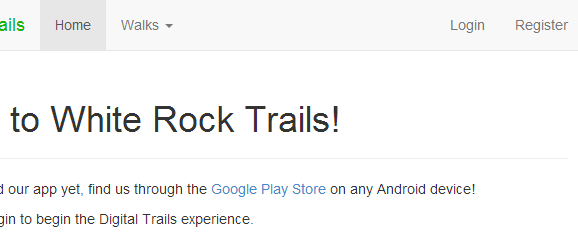
\includegraphics[width=0.7\linewidth]{./img/webportal-guide/login}
\caption{Web portal top navigation bar.}
\label{fig:login-guide}
\end{figure}

\begin{figure}[H]
\centering
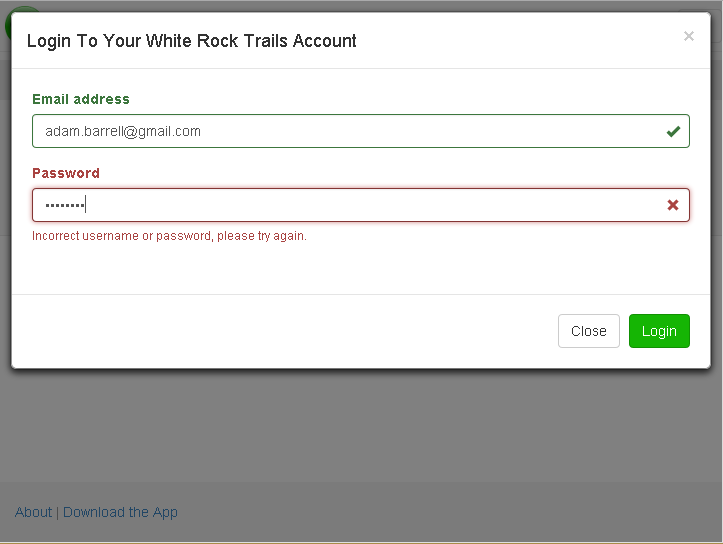
\includegraphics[width=0.6\linewidth]{./img/webportal/login}
\caption{Web portal login modal.}
\label{fig:login-modal}
\end{figure}

\subsubsection{Logging Out}

Log out if you want to prevent other users of your computer being able to access your Digital Trails account.

\begin{enumerate}
\item Click on your full name displayed on the right of the top navigation bar.
\item Click the \emph{logout} button presented in the drop down menu.
\item You are now logged out and the \emph{login} and \emph{register} buttons will replace your full name.
\end{enumerate}

\begin{figure}[h]
\centering
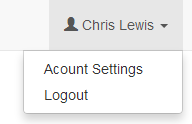
\includegraphics[width=0.4\linewidth]{./img/webportal-guide/logout}
\caption{Web portal logout feature.}
\label{fig:logout}
\end{figure}

\subsubsection{Registering}

Registering an account with the Digital Trails web portal will allow you to gain access to exclusive feature. Such features include the ability to add walks and waypoints.

\begin{enumerate}
\item Click the \emph{register button} from the top navigation bar as shown in Figure \ref{fig:login-guide}.
\item A modal will be displayed which will look similar to that shown in Figure \ref{fig:registration-guide}.
\item Enter your information into the fields on the modal. Your must remember to type your password the same, twice to prevent typing errors.
\item Click the \emph{register} button.
\item If successful, you will be presented with a confirmation dialogue and you will be automatically logged in.
\end{enumerate}

\begin{figure}[H]
\centering
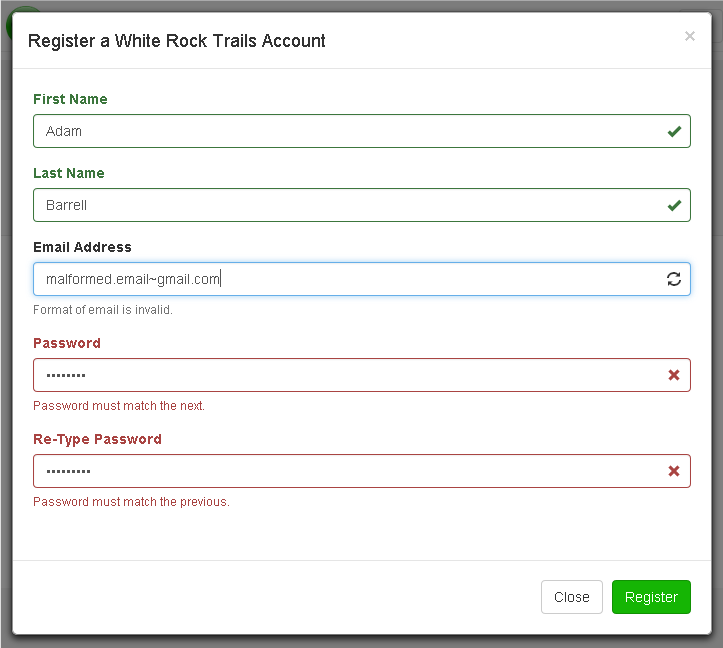
\includegraphics[width=0.6\linewidth]{./img/webportal/registration}
\caption{}
\label{fig:registration-guide}
\end{figure}


\subsubsection{Changing Account Details}

You must first be logged in to change your account details. You may change details such as your \emph{full name}, \emph{email} and \emph{password}.

\begin{enumerate}
\item Once logged in, click on your full name in the top navigation bar.
\item Click the \emph{account settings} option from the drop down menu displayed.
\item You will be navigated to the \emph{account settings} view shown in Figure \ref{fig:user-account-guide} where you should make changes to your account details.
\item When you have made your changes, click the \emph{save} button.
\item If successful, you will be presented with a success confirmation as shown beneath the \emph{save} button in Figure \ref{fig:user-account-guide}.
\end{enumerate}

\begin{figure}[h]
\centering
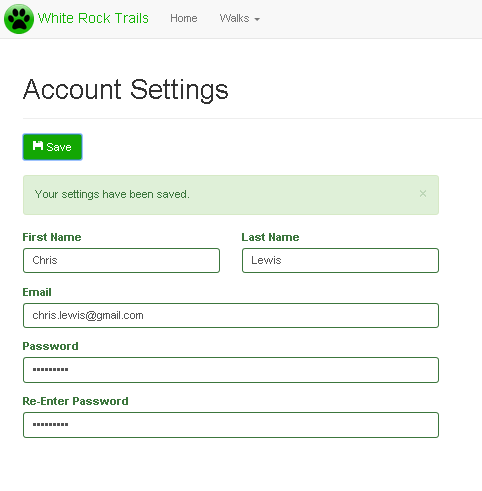
\includegraphics[width=0.7\linewidth]{./img/webportal/user-account}
\caption{Web portal account settings view}
\label{fig:user-account-guide}
\end{figure}

\subsection{Walks}

\subsubsection{Searching Walks}

You can search for walks stored in the Digital Trails database using the instant search feature on the \emph{all walks} or \emph{my walks} view. Use the page indexes shown above and below the walk tiles to change the current page of results.

\begin{enumerate}
\item Navigate to the \emph{all walks} view shown in Figure \ref{fig:all-walks-guide}.
\item Type search criteria into the text box shown beneath the \emph{add walk} button. Your criteria should include text matching a walks title or description.
\item The walk tiles should then change to show only those matching your search criteria.
\end{enumerate}

\begin{figure}[H]
\centering
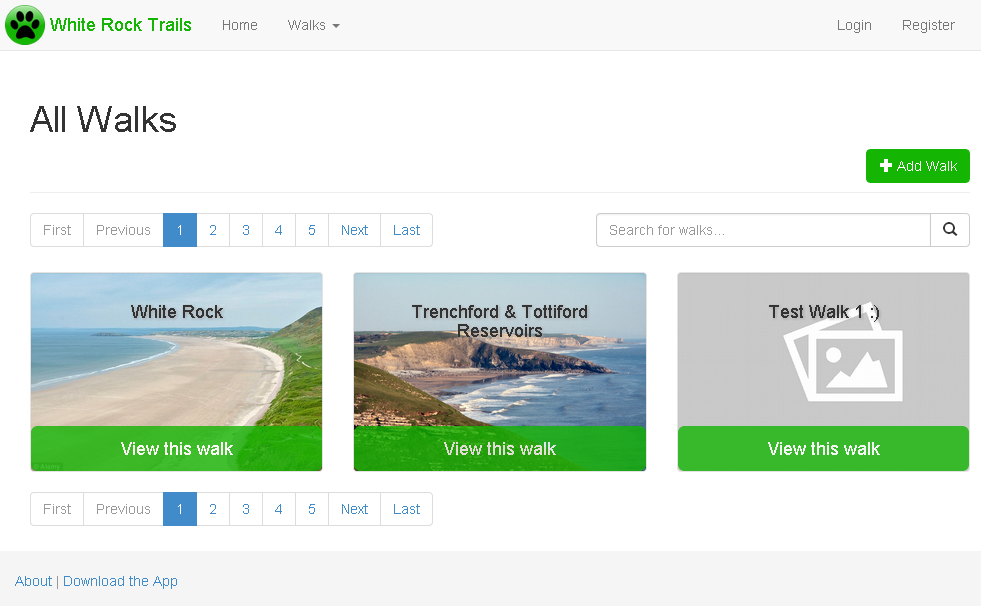
\includegraphics[width=0.8\linewidth]{./img/webportal/all-walks}
\caption{Web portal's walk search feature.}
\label{fig:all-walks-guide}
\end{figure}

\subsubsection{Viewing Walks}

Walks can be viewed to display more information such as a full description, reviews and waypoints.

\begin{enumerate}
\item From the \emph{all walks} or \emph{my walks} views, click the \emph{view this walk} button on a tile of the walk you wish to view.
\item You will be navigated to a walk information page where you can view all details about the walk.
\end{enumerate}

\subsubsection{Adding Walks}

Walks can be added to the Digital Trails database if you have registered an account via the web portal.

\begin{enumerate}
\item Navigate to the \emph{all walks} or \emph{my walks} similar to that shown in Figure \ref{fig:all-walks-guide}.
\item Click the \emph{add walk} button shown above the search box.
\item You will be navigated to the view shown by Figure \ref{fig:add-walk-guide}.
\item Populate the text boxes with the properties of your new walk.
\item Optionally, click a point on the map to add new waypoints to your walk.
\item Once you've finished, click the \emph{create} button to add your new walk to the Digital Trails database.
\end{enumerate}

\begin{figure}[H]
\centering
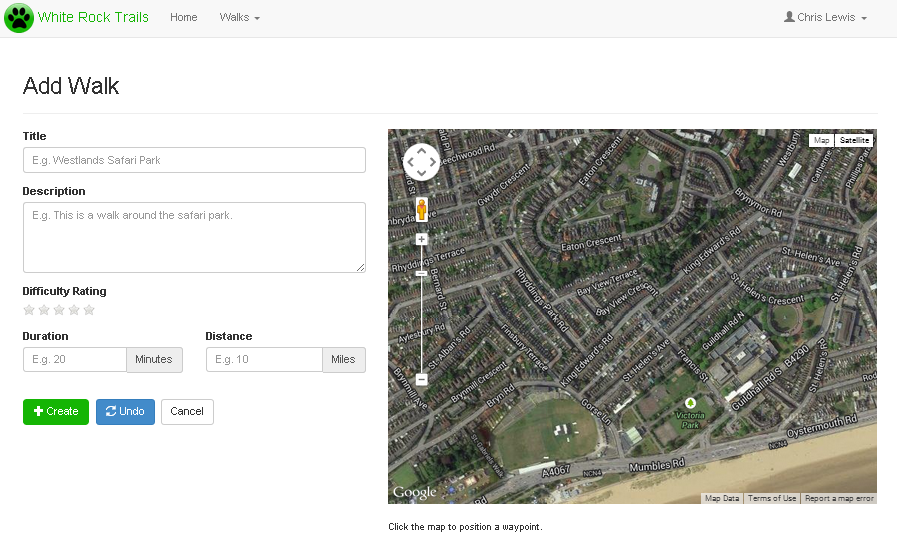
\includegraphics[width=0.8\linewidth]{./img/webportal/add-walk}
\caption{Web portal add walk view.}
\label{fig:add-walk-guide}
\end{figure}

\subsubsection{Editing Walks}

You can edit any of the walks you have previously created if you need to make changes to any information or waypoints associated.

\begin{enumerate}
\item Navigate to the \emph{all walks} or \emph{my walks} view.
\item Click \emph{view this walk} on any walk you have authored.
\item Click the \emph{edit} button on the top right of the view shown in Figure \ref{fig:walk-info-guide}.
\end{enumerate}

\begin{figure}[H]
\centering
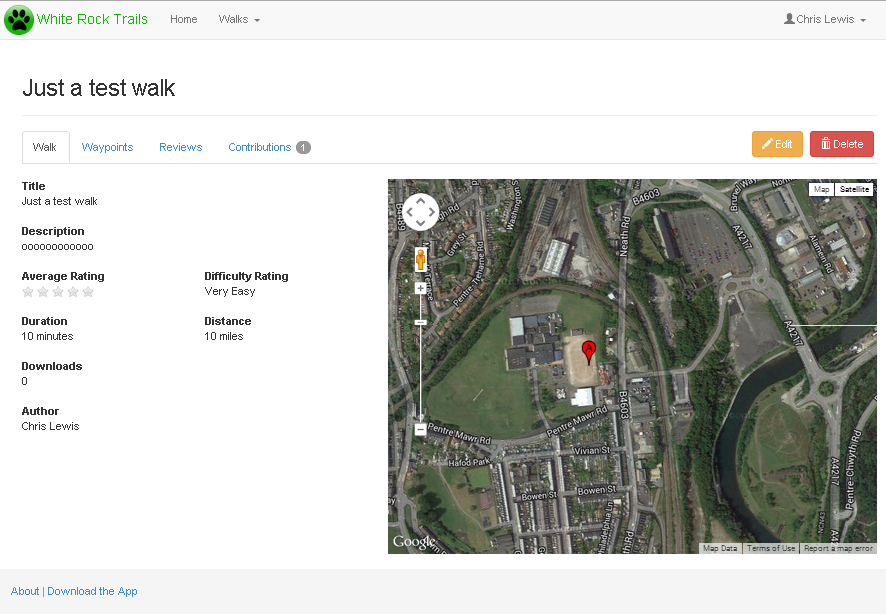
\includegraphics[width=0.8\linewidth]{./img/webportal/walk-info}
\caption{Web portal walk owner perspective.}
\label{fig:walk-info-guide}
\end{figure}

\subsubsection{Deleting Walks}

Any walks that you have created can be deleted and subsequently removed from the Digital Trails database.

\begin{enumerate}
\item Navigate to the \emph{all walks} or \emph{my walks} view.
\item Click \emph{view this walk} on any walk you have authored.
\item Click the \emph{delete} button on the top right of the view shown in Figure \ref{fig:walk-info-guide}.
\end{enumerate}

\subsection{Waypoints}

\subsubsection{Viewing Waypoints}

Waypoints associated to any walk stored in the Digital Trails database can be viewed to display waypoint details and associated media.

\begin{enumerate}
\item Navigate to the \emph{all walks} or \emph{my walks} view.
\item Click \emph{view this walk} on any walk you you wish to view.
\item Click on the \emph{waypoints} tab shown below the walk title in Figure \ref{fig:walk-info-guide}.
\item You will be navigated to the view shown in Figure \ref{fig:walk-waypoints-guide}.
\item Click on a waypoint item from the list or its corresponding map marker.
\item You will be presented with the waypoint modal shown in Figure \ref{fig:walk-waypoints-guide}.
\item Media items can be viewed in full by clicking their preview under the \emph{media gallery} heading.
\end{enumerate}

\begin{figure}[H]
\centering
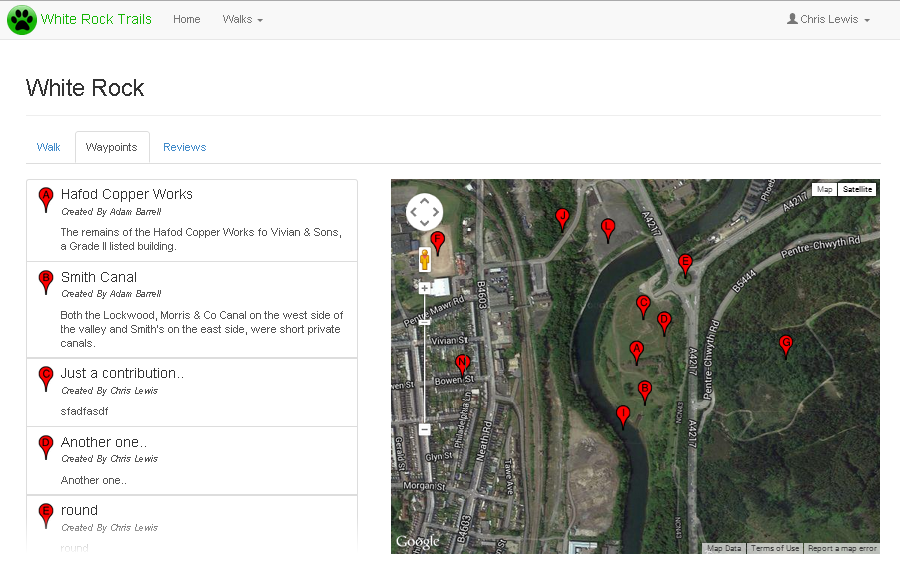
\includegraphics[width=0.8\linewidth]{./img/webportal/walk-waypoints}
\caption{Web portal waypoints list.}
\label{fig:walk-waypoints-guide}
\end{figure}

\begin{figure}[H]
\centering
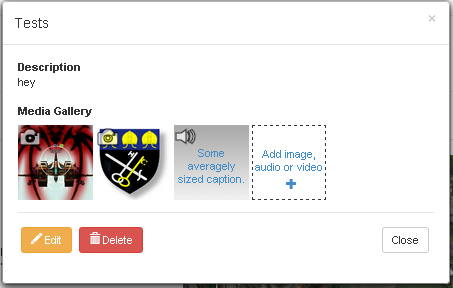
\includegraphics[width=0.7\linewidth]{./img/webportal/waypoint}
\caption{Web portal waypoint view.}
\label{fig:waypoint-guide}
\end{figure}

\subsubsection{Adding Waypoint Media}

Media can be added to waypoints for display in the media gallery. Media items that are allowed to be uploaded are MP4 videos, GIF/JPEG/PNG images and MP3 audio files.

\begin{enumerate}
\item Navigate to the \emph{all walks} or \emph{my walks} view.
\item Click \emph{view this walk} on any walk you you wish to view.
\item Click on the \emph{waypoints} tab shown below the walk title in Figure \ref{fig:walk-info-guide}.
\item You will be navigated to the view shown in Figure \ref{fig:walk-waypoints-guide}.
\item Click on a waypoint item from the list or its corresponding map marker.
\item You will be presented with the waypoint modal shown in Figure \ref{fig:walk-waypoints-guide}.
\item Click the \emph{add image, audio or video} box featuring a dashed border.
\item Double click a media file from your computer using the dialogue shown in Figure \ref{fig:FileUpload}
\item Enter a caption for your media into the modal which is displayed.
\item Your file will be uploaded and added to the collection of waypoint media that already exists.
\end{enumerate}

\begin{figure}[h]
\centering
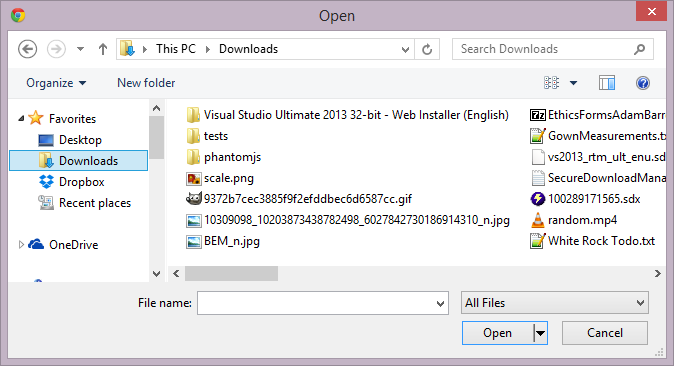
\includegraphics[width=0.7\linewidth]{./img/webportal-guide/FileUpload}
\caption{Web portal file upload dialogue.}
\label{fig:FileUpload}
\end{figure}

\subsubsection{Deleting Waypoint Media}

You must be the owner of a walk in order to delete media from it. Once the media has been deleted, it will be permanently removed from the Digital Trails database.

\begin{enumerate}
\item Navigate to the \emph{all walks} or \emph{my walks} view.
\item Click \emph{view this walk} on any walk you you wish to view.
\item Click on the \emph{waypoints} tab shown below the walk title in Figure \ref{fig:walk-info-guide}.
\item You will be navigated to the view shown in Figure \ref{fig:walk-waypoints-guide}.
\item Click on a waypoint item from the list or its corresponding map marker.
\item You will be presented with the waypoint modal shown in Figure \ref{fig:walk-waypoints-guide}.
\item Click the \emph{edit} button in the bottom left of the modal.
\item An edit waypoint modal should appear, click the \emph{manage} button under the \emph{media manager} heading.
\item A new modal should appear like the one shown in Figure \ref{fig:media-gallery-guide}.
\item Select media items you wish to delete and click the \emph{delete selected} button.
\item 

\begin{figure}[h]
\centering
\includegraphics[width=0.7\linewidth]{./img/webportal/media-gallery}
\caption{Web portal media manager.}
\label{fig:media-gallery-guide}
\end{figure}


\end{enumerate}

\subsubsection{Adding Waypoints}

Waypoints can be added to new or existing walks. If you add a waypoint to a walk created by someone else, it will be added to the walk upon approval by the walk author.

\begin{enumerate}
\item When adding a new walk or viewing an existing one, click on a point on the map where you wish to place the waypoint.
\item The modal displayed in Figure \ref{fig:add-waypoint-guide} will be displayed where you can edit the attributes of your new waypoint.
\item Click the \emph{manage} button to upload media items such as images, videos and audio to the waypoint.
\item When you have finished editing, click the \emph{create} button.
\item The modal will close and you will see your new waypoint added to the walk map.
\end{enumerate}

\begin{figure}[H]
\centering
\includegraphics[width=0.7\linewidth]{./img/webportal/add-waypoint}
\caption{Web portal adding a waypoint.}
\label{fig:add-waypoint-guide}
\end{figure}


\subsubsection{Editing Waypoints}

Existing waypoints can be edited on walks that you have authored. You can edit waypoints to change the information displayed or manage the media uploaded by other users.

\begin{enumerate}
\item When viewing a walk that you have authored, click on a waypoint marker from the map or item from the waypoints list.
\item A waypoint modal will be displayed like the one shown in Figure \ref{fig:waypoint-guide}.
\item Click the \emph{edit} button in the bottom right of the modal.
\item An edit modal will appear similar to that shown in Figure \ref{fig:add-waypoint-guide}.
\item Make any necessary changes to the waypoint attributes using the text fields.
\item Media items uploaded to the waypoint can also be managed by clicking on the \emph{manage} button.
\end{enumerate}

\subsubsection{Deleting Waypoints}

You can delete waypoints from walks that you have authored. This will permanently remove the waypoint from the Digital Trails database and any associated media items.

\begin{enumerate}
\item When viewing a walk that you have authored, click on a waypoint marker from the map or item from the waypoints list.
\item A waypoint modal will be displayed like the one shown in Figure \ref{fig:waypoint-guide}.
\item Click the \emph{delete} button at the bottom left of the modal.
\item When prompted to delete the waypoint, click \emph{yes}.
\item The waypoint will be permanently deleted from the Digital Trails database and subsequently be removed from the map.
\end{enumerate}

\subsection{Walk Contributions}

\subsubsection{Reviewing Waypoint Contributions}

As a walk author, you will be required to accept or reject any waypoints that have been added to your walk by other users. Please note, the \emph{contributions} tab will only be visible if you have at least one contribution to moderate.

\begin{enumerate}
\item Navigate to the \emph{all walks} or \emph{my walks} view.
\item Click \emph{view this walk} on any walk you you wish to view.
\item Click on the \emph{contributions} tab shown below the walk title in Figure \ref{fig:waypoint-contributions-guide}.
\item Click the \emph{accept} or \emph{reject} button within the waypoint description to add or discard the waypoint from your walk respectively.
\item The map will then update to either show or discard your change depending on your choice.
\end{enumerate}

\begin{figure}[H]
\centering
\includegraphics[width=0.8\linewidth]{./img/webportal/waypoint-contributions}
\caption{Web portal contributions view.}
\label{fig:waypoint-contributions-guide}
\end{figure}

\subsubsection{Leaving Walk Reviews}

Reviews can be left on your own or other user's walks which become visible to the public.

\begin{enumerate}
\item Navigate to the \emph{all walks} or \emph{my walks} view.
\item Click \emph{view this walk} on any walk you you wish to view.
\item Click on the \emph{reviews} tab shown below the walk title in Figure \ref{fig:walk-reviews-guide}.
\item Click the \emph{add review} button below the tabs.
\item The list of reviews will collapse and a form will appear.
\item Give your review a title, star rating and description.
\item Click the \emph{save} button below the form.
\item The reviews list will reappear and your review will be added at the top.
\end{enumerate}

\begin{figure}[H]
\centering
\includegraphics[width=0.8\linewidth]{./img/webportal/walk-reviews}
\caption{Web portal walk reviews.}
\label{fig:walk-reviews-guide}
\end{figure}

\subsubsection{Deleting Walk Reviews}

A walk review can be deleted if it is your own, or the review is associated with your walk.

\begin{enumerate}
\item Navigate to the \emph{all walks} or \emph{my walks} view.
\item Click \emph{view this walk} on any walk you you wish to view.
\item Click on the \emph{reviews} tab shown below the walk title in Figure \ref{fig:walk-reviews-guide}.
\item Click the \emph{delete} button inside the review box you wish to delete.
\item Your chosen review will be permanently deleted from the Digital Trails database and it will subsequently be removed from the list.
\end{enumerate}

\section{Android Application}
\label{user_manual_application}

\subsection{Installation}

Section about how to install the application onto your device.

\subsection{Getting started}

INSERT IMAGES\\

To open the White Rock application, navigate to the `Apps' section of your Android device and select the `WhiteRockTrail' thumbnail. When selected, the application will launch and present the \emph{Splash Screen}, shortly followed by the \emph{Launch} interface. Here, you may log in to \emph{White Rock Trails} or continue as a guest. Note: Guest mode has restricted privileges that may prevent you from carrying out certain activities.\\

You are now ready to start using the application. For a quick start tutorial, proceed to section GET SECTION NAME. For a complete tutorial, proceed to section GET SECTION NAME. 

\subsection{Quick start - Create a walk}

In this section, a quick start tutorial will present all necessary steps required to carry out the basic application features. The tutorial will document the following features:-

 \begin{itemize}
   \item Create an account
   \item Create a walk
   \item View a walk
 \end{itemize}

\paragraph*{Create an account}\mbox{}\\

Signing up to White Rock Trails can bring numerous benefits including full access to all application features, monthly newsletters highlighting popular local walks etc. To create an account, select the \emph{Log In} button situated at the centre of the \emph{Launch} interface (figure \ref{fig:launch_viewUM}). This will navigate to the \emph{Log In} interface. If you don't already have an existing account, select the \emph{New user?} text below the \emph{Sign In} button. This will navigate to the \emph{Register} interface GET IMAGE. Here you are required to enter you first and last name, email address and asked to create a password. When you've finished filling in all four text fields, press the \emph{Create Account} button. This will validate the details you have entered, checking whether you may proceed or need to amend your information. If the details entered are valid, the application will create a new user account and navigate to the \emph{Home} interface.

\begin{figure}[H]
    \centering
    \includegraphics[width=0.8\textwidth]{chris/launch_view}
    \caption{Launch interface}
    \label{fig:launch_viewUM}
\end{figure}

\paragraph*{Create a walk}\mbox{}\\

Now that you have a registered account, you may create a new walk. To do so, select the \emph{My Walks} button of the \emph{Home} interface. This will inflate the \emph{My Walks} interface. Next, select the \emph{Create Walk} button, that will navigate to the \emph{Create Walk} interface (figure \ref{fig:create_walkUM}). First, give your walk a name and then add a description as instructed. To create this walk, you must next add a waypoint. Selecting the \emph{Add A Waypoint} button will navigate to the \emph{Add Waypoint} interface, which displays an interaction map and prompt text. Press and holding on a location will create a waypoint at that position. A waypoint dialogue will inflate requesting a waypoint name and description. From this dialogue, the geological location of the waypoint can also be changed, however, this is discouraged and the `drag-and-drop' waypoint feature is preferred. When adding waypoints is complete, selecting the \emph{create} button will create and save the walk. This walk will now appear in the \emph{My Walks} interface, where it may be edited or deleted and also in the \emph{Save Walks} interface, where you may view the walk.

\begin{figure}[H]
    \centering
    \includegraphics[width=0.8\textwidth]{chris/home}
    \caption{Home interface}
    \label{fig:homeUM}
\end{figure}

\begin{figure}[H]
    \centering
    \includegraphics[width=0.8\textwidth]{chris/create_walk}
    \caption{Create Walk interface}
    \label{fig:create_walkUM}
\end{figure}

\paragraph*{View a walk}

Now that you've created a walk, you may view it. At the \emph{Home} interface, select the \emph{Saved Walks} button. Your newly created walk will now appear in the list on the left hand side. To view a walk, select the walk name from the list so that the walk details appear in view, then press the \emph{Start walk} button. This inflates the \emph{Walk View} interface, presenting a full-screen map with walk waypoints. Pressing a waypoint will inflate a pop-up that presents the waypoint name and description. To hide the waypoint details, simply press a different part of the map.

\subsection{Complete application guide}

\chapter{Reflective Account}
\label{sec:reflective-account}
\section{Problem Solving}
\label{sec:problem-solving}
\subsection{Tom Milner - API Development}
\subsection{Adam Barrell - Web Portal Development}

\subsubsection{Third Party Library Bugs}
Bugs were found in a third party library which helped validate user input fields. The library used was called the \emph{bootstrapvalidator}\cite{bootstrapvalidator} created by an open source project. The library utilises the Bootstrap user interface framework to provide styling for valid and invalid fields. Whilst using the library to validate fields in the web portal's login form, a number of bugs were encountered.

The first bug encountered was that the form did not validate when two or more remote API calls were used to check a field's validity. The GIT Hub project discussion forum revealed that this was a known problem and was being fixed by the library's developer. Three days elapsed until the library was fixed and could be used in the web portal login form.

The second bug encountered was more technical and meant that the login form submission method could not be overridden. The presence of this bug however had not been discussed on the project forum. Therefore, I submitted my own bug report specifying the scenario that could be taken to reproduce the problem. Since I has already implemented a solution to this bug, I also specified the code needed to fix it. The project developer quickly replied to the report and the feature was fixed the next day.

\subsubsection{Parallel API Development}
The API and web portal were both developed in parallel, however this brought about some problems during development. The API was being developed separately by Tom Milner and the web portal by Adam Barrell. Nealy all features of the web portal depended entirely upon the API working properly.

Whilst developing the web portal, it was discovered that the API was not functioning correctly when retrieving and manipulating data. One particular example, was when media was uploaded to the server but a thumbnail wasn't generated. This thumbnail was required to allow the media to be previewed in a waypoint media gallery. Therefore, Tom Milner had to fix the problem on the API which in turn, prevented any more development taking place on the media upload feature.

Many similar problems were encountered during development where the API wasn't capable of performing the functions required by the web portal. In addition, API methods were not tested until the system was fully implemented. This meant that many bugs were still present when methods were being consumed by the web portal.

\subsubsection{Client Side Password Hashing}
The web portal login mechanism required passwords to be hashed using a slow hashing algorithm before being sent to the server for account authentication. Slow hashing algorithms make it harder for attackers to decrypt passwords if they are retrieved from the database. When attempting to login with mobile devices, the process was extremely slow. This was because a hashing workload factor had been set such that more powerful desktop computers would hash the password much more quickly than less powerful mobile devices.

A solution was implemented which involved moving the hashing process to the server. This meant that the login process took exactly the same amount of time across devices of varying power.

\subsection{Lewis Hancock - Android Development}
\subsection{Chris Lewis - Android Interface Development}
\section{Learning Experience}
\label{sec:learning-experience}
\subsection{Tom Milner - API Development}
\subsection{Adam Barrell - Web Portal Development}

\subsubsection{Web Technologies}
The main part of my learning experience has been learning new web technologies that I have previously had no experience using. Web applications utilise many different technologies and frameworks depending on the type of application being developed. Although their use is not essential, they make building web applications less time consuming since they provide solutions to many common problems.

AngularJS was the framework that the web portal was built on top of. Learning how to use this framework was a steep learning curve but was significantly reduced by the wealth of documentation and community created tutorials present online. The best approach for the structure and modularisation of JavaScript files was also learned which made the application more maintainable. 

Many technologies concerned with the web portal views such as Twitter Bootstrap and HTML5 were also learned alongside AngularJS. Twitter Bootstrap is a presentation library which contains out-of-the-box styles for HTML components. I learned that using these libraries allowed us to quickly prototype the structure of the web portal views without having to spend time creating custom component styles.

\subsubsection{Working In Parallel}
%reading other peoples code
One of the biggest challenges has been learning to work in parallel with other members of the team. Since Tom Milner was responsible for developing the API, he was an essential asset to the development of the web portal. When I was developing features of the web application, I regularly communicated with Tom to discuss how we could implemented them in both the web portal and API. This was because the web portal needed to consume data from the API which acted as an interface to the database.

Tom and I often partook in pair programming which is promoted by our chosen Agile Scrum methodology. Pair programming involved one of us programming whilst the other observed the code being written. The observers job was to notify the programmer of problems with the code and to suggest potential solutions. This method of programming was adopted when either myself or Tom had an error that we could not fix. With hindsight, it proved to be very effective since we were able to solve most of our programming errors this way.

\subsubsection{User Interface Design}
Another major learning outcome was learning how to develop intuitive interfaces that would be usable by a range of users with varying abilities. Many design principles and patterns were learned from a website called UI-Patterns\cite{uipatterns}. This website listed the most commonly used interface designs to overcome various problems. Such problems included how to display high quantities of data on a page. This was a problem encountered during the design of the \emph{all walks} and \emph{my walks} views. UI-Patterns suggested that a `load on scroll' or pagination technique should be used to prevent too much data being displayed at once. The pagination solution was adopted for use in the mentioned views which allowed users to select a page index to display a subset of the walks returned from the database.

Since the web portal had to be designed for users with varying abilities, a concious effort had to be made to make the interface intuitive enough. The skills learned through doing this can be transferred to any other application that I develop in the future. Therefore, this was a good learning outcome from this project.

\subsection{Lewis Hancock - Android Development}
\subsection{Chris Lewis - Android Interface Development}

\section{Risk Analysis Review}
\label{sec:risk-analysis-review}
\subsection{Anticipated Risks}
\label{sec:anticipated-risks}
\subsection{Un-Anticipated Risks}
\label{sec:unanticipated-risks}
\section{Schedule Review}
\label{sec:schedule-review}
\section{Methodology Review}
\label{sec:methodology-review}
\section{Goals Achieved}
\label{sec:goals-achieved}

\subsection{Tom Milner - API Development}
\subsection{Adam Barrell - Web Portal Development}
\subsection{Lewis Hancock - Android Development}
\subsection{Chris Lewis - Android Interface Development}

\section{Improvements}
\label{sec:improvements}

\subsection{Tom Milner - API Development}
\subsection{Adam Barrell - Web Portal Development}
\subsection{Lewis Hancock - Android Development}
\subsection{Chris Lewis - Android Interface Development}

\section{Individual Contributions}
\label{sec:individual-contributions}

\subsection{Tom Milner - API Development}
\subsection{Adam Barrell - Web Portal Development}
\subsection{Lewis Hancock - Android Development}
\subsection{Chris Lewis - Android Interface Development}

\chapter*{Summary}
\label{sec:summary}
\addcontentsline{toc}{chapter}{Summary}

%References as subsection
\newpage
\bibliographystyle{plain}
\bibliography{bibliography}

\appendix

\end{document}
